\usepackage[utf8]{inputenc}
\usepackage[T1]{fontenc}
% Font A (chosen 2026-09-06): Palatino via newpx for text and math; the
% standalone chapters keep Latin Modern until their own layout pass.
\usepackage{newpxtext}
\usepackage{newpxmath}
% Monospace: TeX Gyre Cursor, the same family as Pagella, scaled to the
% text's lowercase.
% XeTeX computes a native word's height from glyph outlines by default; in
% this document that measurement comes back at about 2.4 em for many
% monospace words (whatever the font), which pushed every line carrying
% \texttt or \path down by a line and a half. With glyph metrics off the
% heights come from the fonts' ascent and descent, which fit the leading, and
% the interline spacing is uniform. Standalone chapters (pdfTeX) are unaffected.
\usepackage{iftex}
\ifXeTeX
  \XeTeXuseglyphmetrics=0
  \usepackage{fontspec}
  % Source Code Pro: dense, with a bold that separates typed input from output
  % in a session; sized to Palatino's lowercase. ItalicFont/BoldItalicFont are
  % declared because \lstdefinestyle{pdcode}'s commentstyle sets \itshape on
  % this family (see below) — without them fontspec has no `m/it` shape to
  % select and silently substitutes upright glyphs for every listing comment,
  % which is exactly the defect this comment used to leave unfixed.
  \setmonofont{SourceCodePro-Regular.otf}[BoldFont=SourceCodePro-Bold.otf,
    ItalicFont=SourceCodePro-RegularIt.otf,BoldItalicFont=SourceCodePro-BoldIt.otf,
    Scale=MatchLowercase]
  % Sans: TeX Gyre Heros, the grotesk the Swiss and technical editions already
  % use for display; without it \textsf falls to Latin Modern Sans.
  \setsansfont{texgyreheros-regular.otf}[ItalicFont=texgyreheros-italic.otf,
    BoldFont=texgyreheros-bold.otf,BoldItalicFont=texgyreheros-bolditalic.otf,
    Scale=MatchLowercase]
  % newpxmath declared its operators font and the \mathrm/\mathsf/\mathtt
  % alphabets before fontspec had set the faces, so every digit, \log, \max
  % and text subscript in math, and every pgfplots tick numeral, was set in
  % Latin Modern while the words around it were Palatino. The faces are
  % declared here under fixed NFSS family names and the math alphabets bound
  % to those names (the \rmdefault indirection resolved to Latin Modern).
  \newfontfamily\pdmathtextface{TeXGyrePagellaX-Regular.otf}[BoldFont=TeXGyrePagellaX-Bold.otf,
    ItalicFont=TeXGyrePagellaX-Italic.otf,BoldItalicFont=TeXGyrePagellaX-BoldItalic.otf,
    NFSSFamily=pdpag]
  \newfontfamily\pdmathsansface{texgyreheros-regular.otf}[BoldFont=texgyreheros-bold.otf,
    Scale=MatchLowercase,NFSSFamily=pdher]
  \newfontfamily\pdmathmonoface{SourceCodePro-Regular.otf}[BoldFont=SourceCodePro-Bold.otf,
    Scale=MatchLowercase,NFSSFamily=pdscp]
  \SetSymbolFont{operators}{normal}{TU}{pdpag}{m}{n}
  \SetSymbolFont{operators}{bold}{TU}{pdpag}{b}{n}
  \SetMathAlphabet{\mathrm}{normal}{TU}{pdpag}{m}{n}
  \SetMathAlphabet{\mathbf}{normal}{TU}{pdpag}{b}{n}
  \SetMathAlphabet{\mathit}{normal}{TU}{pdpag}{m}{it}
  \SetMathAlphabet{\mathsf}{normal}{TU}{pdher}{m}{n}
  \SetMathAlphabet{\mathtt}{normal}{TU}{pdscp}{m}{n}
  % The part openers set their display type in Times (the cover's face). Under
  % fontspec the legacy \fontfamily{ptm} has no TU italic or small caps, so the
  % face is declared here, with both.
  \newfontfamily\pdpartface{texgyretermes-regular.otf}[ItalicFont=texgyretermes-italic.otf,
    BoldFont=texgyretermes-bold.otf,BoldItalicFont=texgyretermes-bolditalic.otf,Ligatures=TeX]
  \newfontfamily\pdgrotesk{texgyreheros-regular.otf}[ItalicFont=texgyreheros-italic.otf,
    BoldFont=texgyreheros-bold.otf,BoldItalicFont=texgyreheros-bolditalic.otf,Ligatures=TeX]
  % A 66-character column cannot hold a script path in one piece. Inside
  % \texttt, XeTeX's inter-character tokens allow a break (no hyphen) after
  % / _ . - = : and , so paths and flags wrap where a reader expects.
  \makeatletter
  \newXeTeXintercharclass\pd@brk
  \XeTeXcharclass`\/=\pd@brk \XeTeXcharclass`\_=\pd@brk \XeTeXcharclass`\.=\pd@brk
  \XeTeXcharclass`\-=\pd@brk \XeTeXcharclass`\==\pd@brk \XeTeXcharclass`\:=\pd@brk \XeTeXcharclass`\,=\pd@brk
  \XeTeXinterchartoks\pd@brk 0={\allowbreak}
  \XeTeXinterchartoks\pd@brk\pd@brk={\allowbreak}
  \expandafter\let\expandafter\pd@texttt\csname texttt \endcsname
  \expandafter\def\csname texttt \endcsname#1{{\XeTeXinterchartokenstate=1 \pd@texttt{#1}}}
  \makeatother
\else
  \newcommand\pdpartface{\fontfamily{ptm}\selectfont}
  \newcommand\pdgrotesk{\fontfamily{qhv}\selectfont}
  % pdfTeX fallback (not the published path; scripts/build-whitepapers.sh
  % compiles the Book with xelatex): the same face through its Type 1 package.
  \usepackage[scale=0.92]{sourcecodepro}
\fi
\let\openbox\relax
\usepackage[fontsize=10.5pt]{fontsize}
\usepackage{microtype}
\usepackage{geometry}
\usepackage{amsmath,amsthm}
\usepackage{listings}
\usepackage{xcolor}
\usepackage{booktabs}
% colortbl is loaded for one reason: \arrayrulecolor, so the concordance table
% at the foot of the chapter map can take a part hue on its booktabs rules
% instead of black. It changes nothing else -- its default rule colour is the
% black every other table in the Book already draws.
\usepackage{colortbl}
\usepackage{tabularx}
\usepackage{xltabular}
\usepackage{array}
\usepackage{graphicx}
\usepackage{fancyhdr}
\usepackage{tikz}
\usepackage{float}
% Page discipline for the Book. Every figure and table in the chapter sources
% asks for [H]; at a 7 x 10 trim that strands a third of a page whenever the
% next exhibit does not fit. In the Book an [H] becomes [!htbp]: the exhibit
% is still set here when it fits and otherwise floats to the top of the next
% page while the text flows on, and a FloatBarrier at every section keeps it
% inside its section. Headings need room for three lines beneath them.
\usepackage[section]{placeins}
\makeatletter
\let\pd@orig@xfloat\@xfloat
\def\@xfloat#1[#2]{\edef\@tempa{#2}\def\@tempb{H}%
  \ifx\@tempa\@tempb\pd@orig@xfloat#1[!htbp]\else\pd@orig@xfloat#1[#2]\fi}
\makeatother
\usepackage{needspace}
\usepackage{etoolbox}
% ---------------------------------------------------------------------------
% Heading weights, in tandem with the contents (titlesec + titletoc).
%
% The contents pages carry their hierarchy in WEIGHT, not size: heavy grotesk
% for chapter titles and part labels, a light italic serif for the one-line
% claims. A reader who learns that grammar on page v should meet the same
% grammar in the body, so the section heads are set in the same grotesk the
% part and chapter openers already use (TeX Gyre Heros, bound at the top of
% this file for all three editions; no new family is introduced).
%
% Sizes step DOWN from the article defaults -- 13.5/11.5/10.5 against
% 14.4/12/10.5 -- because Heros sets wider than Pagella at the same nominal
% size and the column is only 4.5 in. The separation between levels is carried
% by weight and by the space above, which is what the contents does too.
%
% The SPACING, on the other hand, is article's own, to the tenth of an ex, and
% that is deliberate. A first pass tightened it (3.0/1.5, 2.6/1.1, 2.2/0.9) and
% took three pages out of the Book. Those three pages are 500 pages of
% reflow, and a margin note has nowhere to go when the column beneath it
% fills: scripts/harbor-research/page_overflow.py found an exercise pointer,
% a margin portrait and a citation pushed off the bottom of the paper on
% pages 63, 71 and 338, which is a failing check in whitepaper-build and, more
% to the point, ink a reader cannot read. Keeping article's skips makes the
% heading change vertically neutral: the Book is the same 549 pages it was,
% and page_overflow reports zero rows with loss in all three editions. The
% weight and the face are what change; where the type falls does not.
%
% Ordering matters here and is not incidental: titlesec redefines \section and
% friends outright, so it must be loaded and every \titleformat issued BEFORE
% the \pretocmd calls below, or the \Needspace patch is applied to a \section
% that titlesec then throws away. The failure branch of each \pretocmd writes
% to the log so a future reordering cannot break this silently.
% ---------------------------------------------------------------------------
\usepackage{titlesec}
\usepackage{titletoc}
\titleformat{\section}[block]
  {\pdgrotesk\bfseries\fontsize{13.5}{16}\selectfont\color{hhink}\raggedright}
  {\thesection}{0.7em}{}
\titleformat{\subsection}[block]
  {\pdgrotesk\bfseries\fontsize{11.5}{14}\selectfont\color{hhink}\raggedright}
  {\thesubsection}{0.6em}{}
\titleformat{\subsubsection}[block]
  {\pdgrotesk\bfseries\fontsize{10.5}{13}\selectfont\color{hhink}\raggedright}
  {\thesubsubsection}{0.55em}{}
\titlespacing*{\section}{0pt}{3.5ex plus 1ex minus .2ex}{2.3ex plus .2ex}
\titlespacing*{\subsection}{0pt}{3.25ex plus 1ex minus .2ex}{1.5ex plus .2ex}
\titlespacing*{\subsubsection}{0pt}{3.25ex plus 1ex minus .2ex}{1.5ex plus .2ex}
% \paragraph is deliberately left alone: it is a run-in lead-in used hundreds
% of times through the chapters, not a level of the contents' hierarchy.
% The reservation has to cover the heading's own apparatus before it covers any
% prose: a \section spends roughly 3.5 baselines on beforeskip, the heading line
% at \Large and afterskip, so 6 left about 2.5 lines of text under it -- right on
% the two-line rule page_spills enforces, and under it once the glue stretched.
% 5.5 (§5.5, The three subsystems of continuity) and 7.7.5 (Pricing the Bond) landed
% stranded that way in all three editions. 8 and 7 leave four clear lines, which
% is a margin rather than a coin flip, and holds for the Swiss and technical
% editions too, where Heros sets the heads larger than Pagella does.
\pretocmd{\section}{\Needspace*{8\baselineskip}}{}{\GenericWarning{}{pd-book: \string\pretocmd\space on \string\section\space FAILED -- heading orphan protection is off}}
\pretocmd{\subsection}{\Needspace*{7\baselineskip}}{}{\GenericWarning{}{pd-book: \string\pretocmd\space on \string\subsection\space FAILED}}
\pretocmd{\subsubsection}{\Needspace*{7\baselineskip}}{}{\GenericWarning{}{pd-book: \string\pretocmd\space on \string\subsubsection\space FAILED}}
\usepackage{caption}
\usepackage{enumitem}
\usepackage{refcount}
\usepackage{eso-pic}   % full-bleed jacket plate behind the title page
\usepackage[backref=page]{hyperref}
\usetikzlibrary{arrows.meta,positioning,fit,backgrounds,calc,shapes.geometric,shapes.symbols,decorations.pathmorphing,decorations.pathreplacing}
% Regime figures in the chapters (the sealed room's composition crossover and
% operating curve, and any later pgfplots fragment) need the axis environment
% in the Book as well as in the standalones.
\usepackage{pgfplots}
\pgfplotsset{compat=1.18}

% Trim 7 x 10 in (Wave 12, L1): one text column of 4.5 in (about 66 characters
% at 10.5 pt) and a 1.3 in outer margin column that carries sidenotes, margin
% heads, exercise pointers and margin figures. The standalone chapters keep A4.
% ---------------------------------------------------------------------------
% Editions. One set of chapter sources, three characters: maritime (the
% watercolour plates), swiss (colour blocking, grotesk display, flat marks) and
% technical (the Seventies manual: monoline ink, halftone, one warm accent,
% drawing-sheet openers). A driver root sets \pdedition before \input-ing the
% Book; without one, the Book takes the default set on the next line.
%
% Swiss is the central edition. The canonical artifact --
% coordination-papers-mega-volume.pdf, the file every published link on the
% site already points at -- renders Swiss because this default says so, which
% is the whole of the switch: no path, no link and no registry entry moves
% when the central edition changes, only this macro.
%
% Maritime and technical remain switchable and are NOT built for now. Their
% driver roots (coordination-papers-mega-volume-{maritime,technical}.tex),
% their plates and their branches in this preamble and in the root all stay in
% the tree, so either one still builds by hand:
%
%   scripts/build-whitepapers.sh coordination-papers-mega-volume-maritime
%
% They are simply out of the default build list in scripts/build-whitepapers.sh
% (see UNBUILT_EDITIONS there) and out of the published registry, because
% nothing publishes them today.
% ---------------------------------------------------------------------------
\providecommand{\pdedition}{swiss}
\newif\ifpdmaritime\newif\ifpdswiss\newif\ifpdtechnical
\makeatletter
\edef\pd@ed{\pdedition}
\def\pd@tmp{maritime}\ifx\pd@ed\pd@tmp\pdmaritimetrue\fi
\def\pd@tmp{swiss}\ifx\pd@ed\pd@tmp\pdswisstrue\fi
\def\pd@tmp{technical}\ifx\pd@ed\pd@tmp\pdtechnicaltrue\fi
\makeatother
% The technical edition's accents are the brand's own Seventies trio: amber
% (mustard), rust (brown) and gold (avocado); no colour outside the palette.
\geometry{paperwidth=7in,paperheight=10in,left=0.8in,right=1.7in,%
  top=0.85in,bottom=0.95in,textwidth=4.5in,marginparsep=0.2in,marginparwidth=1.3in}
\captionsetup{font=small,labelfont=bf}
\setlength{\emergencystretch}{3em}\tolerance=1500
% Depth 1 (parts, chapters, and top-level sections) is a deliberate choice for
% a book assembled from independently structured chapters: at depth 2 the
% front-matter ToC runs to several hundred headings and reads as a text-only
% index rather than a map. Each chapter's own reader's map / abstract is the
% fine-grained entry point; this ToC's job is to show the four parts, the
% chapter spine, and the appendices. The PDF bookmarks go three levels deep.
\setcounter{tocdepth}{1}
\makeatletter
% article.cls has no chapter level; the Book adds one between part and section.
\providecommand*{\toclevel@chapter}{0}
\makeatother
% ---------------------------------------------------------------------------
% The contents, set with titletoc. NO DOT LEADERS ANYWHERE.
%
% What the default engine does, and why it is wrong here: \@dottedtocline sets
% the entry, then a rubber-length run of dots, then the page number in a box
% at the right margin. The reader's eye has to travel the whole measure and
% come back, once per line, and the dots are a rail built to make that travel
% survivable. Remove the travel and the rail has no work left.
%
% So the page number is set 0.6 em after the entry text -- close enough that
% the title and its numeral read as ONE data block -- and the line then simply
% stops, ragged right. That leaves a soft right edge and a hard left one:
% every entry, at every level, hangs from a single left vertical datum, and
% each level's continuation lines return to that level's own datum. No
% centring and no justification: the asymmetry is the point.
%
% Weight, not size, separates the levels, matching the \titleformat block
% above and the chapter map below: grotesk bold for parts and chapters,
% grotesk regular at a smaller optical size and a muted ink for sections.
% ---------------------------------------------------------------------------
\titlecontents{part}[0pt]
  {\addvspace{1.5em}\pdgrotesk\bfseries\fontsize{11.5}{14}\selectfont\color{hhink}}
  {}{}
  {\hspace{0.6em}\normalfont\pdgrotesk\fontsize{9}{11}\selectfont\color{hhgray}\thecontentspage}
  [\addvspace{0.45em}]
\titlecontents{chapter}[1.9em]
  {\addvspace{0.8em}\pdgrotesk\bfseries\fontsize{10.5}{13}\selectfont\color{hhink}}
  {\contentslabel{1.9em}}
  {\hspace*{-1.9em}}
  {\hspace{0.6em}\normalfont\pdgrotesk\fontsize{9}{11}\selectfont\color{hhgray}\thecontentspage}
  [\addvspace{0.15em}]
% Numberless entries (front matter, "Review of the key ideas", the per-chapter
% appendix heads) keep the SAME text datum as numbered ones -- an empty
% numberless format, not a negative kern back to the margin. A section that
% happens to carry no numeral is still a section, and letting it jump to the
% left margin is what broke the left axis in the default engine's output.
\titlecontents{section}[3.4em]
  {\pdgrotesk\fontsize{9}{11.6}\selectfont\color{pdinkmuted}}
  {\contentslabel{2.3em}}
  {}
  {\hspace{0.55em}\color{hhgray}\thecontentspage}
\titlecontents{subsection}[5.9em]
  {\pdgrotesk\fontsize{8.5}{11}\selectfont\color{pdinkmuted}}
  {\contentslabel{2.6em}}
  {}
  {\hspace{0.55em}\color{hhgray}\thecontentspage}
\titlecontents{subsubsection}[8.7em]
  {\pdgrotesk\fontsize{8.5}{11}\selectfont\color{pdinkmuted}}
  {\contentslabel{2.9em}}
  {}
  {\hspace{0.55em}\color{hhgray}\thecontentspage}
\titlecontents{figure}[3.4em]
  {\pdgrotesk\fontsize{9}{11.6}\selectfont\color{pdinkmuted}}
  {\contentslabel{2.6em}}
  {}
  {\hspace{0.55em}\color{hhgray}\thecontentspage}
\titlecontents{table}[3.4em]
  {\pdgrotesk\fontsize{9}{11.6}\selectfont\color{pdinkmuted}}
  {\contentslabel{2.6em}}
  {}
  {\hspace{0.55em}\color{hhgray}\thecontentspage}

\definecolor{codebg}{RGB}{248,248,248}
\definecolor{codeframe}{RGB}{200,200,200}
\definecolor{darkgreen}{HTML}{00564C}
\definecolor{darkblue}{HTML}{003FB8}
\definecolor{accent}{HTML}{00564C}
\definecolor{hhsand}{HTML}{E9DCC4}
\definecolor{hhsanddeep}{HTML}{D8C7A6}
\definecolor{hhebony}{HTML}{121212}
\definecolor{hhink}{HTML}{1B1712}
\definecolor{hhcobalt}{HTML}{003FB8}
\definecolor{hhamber}{HTML}{6B4500}
\definecolor{hhteal}{HTML}{00564C}
\definecolor{hhpaper}{HTML}{FBF7EF}
\definecolor{hhgray}{HTML}{5C5650}
% The Book's semantic color system: palette v2, light values. One hue, one meaning.
% Source of record for every hex: website-v2/src/styles/tokens.semantic.css (light
% theme); website-v2/scripts/check-figure-palette.mjs fails the build if this file
% and the tokens disagree. Twin copy under whitepaper/figures/ (byte-identical).
%
% Separation: contrast says an ink is READABLE on the cream; it says nothing about
% whether two inks are TELLABLE APART, and until now only the first was checked.
% check-figure-palette-separation.mjs measures all 21 pairs in OKLab with protanopia
% and deuteranopia simulated. indigo and violet are re-stepped (deeper, on their own
% hues, both gaining contrast) because they were the pairs with room: cobalt/indigo
% was dE 9.1 and is 15.1; cobalt/violet collapsed to 4.8 under protanopia and is 8.6.
% Three pairs CANNOT be fixed -- teal/health, gold/health and teal/gold have ceilings
% of 12.2, 13.9 and 14.3 against a floor of 15, because sRGB has no chroma to spend
% on the 112-182 degree arc this dark. Only ONE of gold, health and teal may carry a
% series by colour alone; the others need a label, a gap, or a texture.
%
% Discipline: story colors are accents (rules, fills, marks, display text); body
% pages stay cream and ink. Amber is stripes, dots, and display only, never small
% text (3.71:1 on cream). Violet and gold are AA as text; use them at display size
% or on rules and fills. Line weights: 1px texture, 1.5px linework, 2px enclosure.
\definecolor{pdcobalt}{HTML}{003FB8}      % kernel / truth            --brand-primary
\definecolor{pdteal}{HTML}{006B5F}        % legibility                --brand-accent
\definecolor{pdhealth}{HTML}{1F7A4D}      % ready / coordinated       --story-health
\definecolor{pdindigo}{HTML}{312865}      % protocol / federation     --story-indigo
\definecolor{pdviolet}{HTML}{822586}      % identity / continuity     --story-violet
\definecolor{pdrust}{HTML}{7A4514}        % reputation / trust earned --story-rust
\definecolor{pdgold}{HTML}{666A00}        % economy / value           --story-gold
\definecolor{pderror}{HTML}{BF2F2F}       % breach / correction       --status-error
\definecolor{pdamber}{HTML}{A66F00}       % warning (display only)    --status-warning
\definecolor{pdlime}{HTML}{CAD900}        % highlight fill, ink text  --chart-yellow
\definecolor{pdink}{HTML}{121212}         % ink                       --text-primary
\definecolor{pdinkmuted}{HTML}{403B34}    % links, secondary text     --text-secondary
\definecolor{pdcream}{HTML}{F2EEE6}       % page ground               --surface-base
\definecolor{pdcreamraised}{HTML}{F7F3EB} % panels                    --surface-raised
\definecolor{pdcreamstrong}{HTML}{E9E2D5} % inset wells               --surface-strong
% Print inks for the Swiss edition of the Book (SWISS-BRIEF, B); print only.
\definecolor{pdswissblue}{HTML}{001489}
\definecolor{pdswissviolet}{HTML}{582C83}
\definecolor{pdswissred}{HTML}{DA291C}
% And the maritime edition's fourth ink: antique gold, the trim of the engraved
% plates carried onto the page (opener rules, part-title ornament, fillets round
% framed matter). Flat stand-in for a metallic pass; print only.
\definecolor{pdmaritimegold}{HTML}{805A14}

% GENERATED FILE. Do not edit by hand.
% Source of record: whitepaper/textbook.json (chapter order, numbers, parts, edition).
% Regenerate both committed copies: node scripts/generate-mega-whitepaper.mjs --sync-shared
% Drift check (CI): node --test scripts/generate-mega-whitepaper.test.mjs
% Twin copies: whitepaper/figures/pd-textbook-map.tex and
%              website-v2/public/whitepaper/figures/pd-textbook-map.tex (byte-identical).
%
% Every standalone chapter preamble defines \pdchapterprefix before inputting
% this file; the Book redefines it at every \pdchapter. Everything else derives.

\providecommand{\pdeditiontitle}{The Harbor, the Person, and the Economy}
\providecommand{\pdeditionsubtitle}{A textbook of accountable autonomous work}
\providecommand{\pdeditionversion}{4.0 (Textbook Edition)}
\providecommand{\pdeditiondate}{September 2026}
\providecommand{\pdeditionclaim}{Autonomy scales only when authority, evidence, and consequence remain coupled at every effect boundary.}
\providecommand{\pdbooktitle}{\emph{\pdeditiontitle}}
\providecommand{\pdchaptercount}{8}
\providecommand{\pdchaptercountword}{eight}
\providecommand{\pdpartcount}{4}
\providecommand{\pdchapterprefix}{none}
\expandafter\providecommand\csname pdchapternumberofnone\endcsname{0}
\expandafter\providecommand\csname pdchaptertitleofnone\endcsname{\pdeditiontitle}
\expandafter\providecommand\csname pdchaptercolorofnone\endcsname{pdcobalt}
\expandafter\providecommand\csname pdchapternumberofswk\endcsname{1}
\expandafter\providecommand\csname pdchaptertitleofswk\endcsname{The Single-Writer Kernel}
\expandafter\providecommand\csname pdchaptercolorofswk\endcsname{pdcobalt}
\expandafter\providecommand\csname pdchapterformerofswk\endcsname{II}
\expandafter\providecommand\csname pdchapterpartindexofswk\endcsname{1}
\expandafter\providecommand\csname pdchapterpartlabelofswk\endcsname{Part I \textperiodcentered\ Ground Truth}
\expandafter\providecommand\csname pdchapterquestionofswk\endcsname{Where can a rule be made real?}
\expandafter\providecommand\csname pdchapteronelineofswk\endcsname{One writer, one durable file, decides what is true so nothing above it has to guess.}
\expandafter\providecommand\csname pdchapterepigraphofswk\endcsname{A distributed system is one in which the failure of a computer you didn't even know existed can render your own computer unusable.}
\expandafter\providecommand\csname pdchapterepigraphsourceofswk\endcsname{Leslie Lamport, message to a DEC SRC bulletin board, 28 May 1987}
\expandafter\providecommand\csname pdchapternumberofanchor\endcsname{2}
\expandafter\providecommand\csname pdchaptertitleofanchor\endcsname{The Anchor Protocol}
\expandafter\providecommand\csname pdchaptercolorofanchor\endcsname{pdcobalt}
\expandafter\providecommand\csname pdchapterformerofanchor\endcsname{V}
\expandafter\providecommand\csname pdchapterpartindexofanchor\endcsname{1}
\expandafter\providecommand\csname pdchapterpartlabelofanchor\endcsname{Part I \textperiodcentered\ Ground Truth}
\expandafter\providecommand\csname pdchapterquestionofanchor\endcsname{How may authority travel without silently growing?}
\expandafter\providecommand\csname pdchapteronelineofanchor\endcsname{Delegated capability only narrows: every child is a subset of its parent, at every hop, and the verifier checks the whole chain.}
\expandafter\providecommand\csname pdchapterepigraphofanchor\endcsname{Every program and every user of the system should operate using the least set of privileges necessary to complete the job.}
\expandafter\providecommand\csname pdchapterepigraphsourceofanchor\endcsname{Jerome Saltzer and Michael Schroeder, The Protection of Information in Computer Systems, 1975}
\expandafter\providecommand\csname pdchapternumberofsealed\endcsname{3}
\expandafter\providecommand\csname pdchaptertitleofsealed\endcsname{The Sealed Harbor}
\expandafter\providecommand\csname pdchaptercolorofsealed\endcsname{pdcobalt}
\expandafter\providecommand\csname pdchapterformerofsealed\endcsname{}
\expandafter\providecommand\csname pdchapterpartindexofsealed\endcsname{1}
\expandafter\providecommand\csname pdchapterpartlabelofsealed\endcsname{Part I \textperiodcentered\ Ground Truth}
\expandafter\providecommand\csname pdchapterquestionofsealed\endcsname{What can a sealed agent leak, and how would we know?}
\expandafter\providecommand\csname pdchapteronelineofsealed\endcsname{A work order runs in a room with two fences and two gates, the only thing that leaves is what the slot lets out, and the budget of what can leak is a ledger that conserves.}
\expandafter\providecommand\csname pdchapterepigraphofsealed\endcsname{Whereof one cannot speak, thereof one must be silent.}
\expandafter\providecommand\csname pdchapterepigraphsourceofsealed\endcsname{Ludwig Wittgenstein, Tractatus Logico-Philosophicus, proposition 7, 1921 (Ogden translation, 1922)}
\expandafter\providecommand\csname pdchapternumberofls\endcsname{4}
\expandafter\providecommand\csname pdchaptertitleofls\endcsname{The Legible Swarm}
\expandafter\providecommand\csname pdchaptercolorofls\endcsname{pdteal}
\expandafter\providecommand\csname pdchapterformerofls\endcsname{I}
\expandafter\providecommand\csname pdchapterpartindexofls\endcsname{2}
\expandafter\providecommand\csname pdchapterpartlabelofls\endcsname{Part II \textperiodcentered\ The Cost of Seeing}
\expandafter\providecommand\csname pdchapterquestionofls\endcsname{What must remain visible, and what does seeing cost?}
\expandafter\providecommand\csname pdchapteronelineofls\endcsname{The operator's problem is blindness, not collision; supervision has an information cost you can price in bits.}
\expandafter\providecommand\csname pdchapterepigraphofls\endcsname{Certain forms of knowledge and control require a narrowing of vision. The great advantage of such tunnel vision is that it brings into sharp focus certain limited aspects of an otherwise far more complex and unwieldy reality.}
\expandafter\providecommand\csname pdchapterepigraphsourceofls\endcsname{James C. Scott, Seeing Like a State, 1998}
\expandafter\providecommand\csname pdchapternumberofstp\endcsname{5}
\expandafter\providecommand\csname pdchaptertitleofstp\endcsname{From Spawn to Person}
\expandafter\providecommand\csname pdchaptercolorofstp\endcsname{pdviolet}
\expandafter\providecommand\csname pdchapterformerofstp\endcsname{III}
\expandafter\providecommand\csname pdchapterpartindexofstp\endcsname{3}
\expandafter\providecommand\csname pdchapterpartlabelofstp\endcsname{Part III \textperiodcentered\ What Survives the Restart}
\expandafter\providecommand\csname pdchapterquestionofstp\endcsname{What remains long enough to owe anything?}
\expandafter\providecommand\csname pdchapteronelineofstp\endcsname{Continuity turns an anonymous spawn into a ledger position with a witnessed record; reputation is what that record is worth.}
\expandafter\providecommand\csname pdchapterepigraphofstp\endcsname{Person, as I take it, is the name for this self. It is a forensic term, appropriating actions and their merit; and so belongs only to intelligent agents, capable of a law, and happiness, and misery.}
\expandafter\providecommand\csname pdchapterepigraphsourceofstp\endcsname{John Locke, An Essay Concerning Human Understanding, II.xxvii.26, 1690}
\expandafter\providecommand\csname pdchapternumberofhe\endcsname{6}
\expandafter\providecommand\csname pdchaptertitleofhe\endcsname{The Harbor Economy}
\expandafter\providecommand\csname pdchaptercolorofhe\endcsname{pdgold}
\expandafter\providecommand\csname pdchapterformerofhe\endcsname{IV}
\expandafter\providecommand\csname pdchapterpartindexofhe\endcsname{4}
\expandafter\providecommand\csname pdchapterpartlabelofhe\endcsname{Part IV \textperiodcentered\ Trade Between Strangers}
\expandafter\providecommand\csname pdchapterquestionofhe\endcsname{What makes cooperation rational without making loss unbounded?}
\expandafter\providecommand\csname pdchapteronelineofhe\endcsname{Once records cannot be minted, trust can be rented between operators who never met: a three-sided market on one conserving ledger.}
\expandafter\providecommand\csname pdchapterepigraphofhe\endcsname{Virtually every commercial transaction has within itself an element of trust, certainly any transaction conducted over a period of time.}
\expandafter\providecommand\csname pdchapterepigraphsourceofhe\endcsname{Kenneth J. Arrow, Gifts and Exchanges, 1972}
\expandafter\providecommand\csname pdchapternumberofbonded\endcsname{7}
\expandafter\providecommand\csname pdchaptertitleofbonded\endcsname{The Bonded Commons}
\expandafter\providecommand\csname pdchaptercolorofbonded\endcsname{pdgold}
\expandafter\providecommand\csname pdchapterformerofbonded\endcsname{VI}
\expandafter\providecommand\csname pdchapterpartindexofbonded\endcsname{4}
\expandafter\providecommand\csname pdchapterpartlabelofbonded\endcsname{Part IV \textperiodcentered\ Trade Between Strangers}
\expandafter\providecommand\csname pdchapterquestionofbonded\endcsname{Who may decide, on what evidence, with what consequence?}
\expandafter\providecommand\csname pdchapteronelineofbonded\endcsname{Bonds, witnesses, audits and appeals turn residual uncertainty into an institution; the ledger's conservation law is mechanically checked.}
\expandafter\providecommand\csname pdchapterepigraphofbonded\endcsname{If men were angels, no government would be necessary. If angels were to govern men, neither external nor internal controls on government would be necessary.}
\expandafter\providecommand\csname pdchapterepigraphsourceofbonded\endcsname{James Madison, Federalist No. 51, 1788}
\expandafter\providecommand\csname pdchapternumberoffh\endcsname{8}
\expandafter\providecommand\csname pdchaptertitleoffh\endcsname{The Federated Harbor}
\expandafter\providecommand\csname pdchaptercoloroffh\endcsname{pdgold}
\expandafter\providecommand\csname pdchapterformeroffh\endcsname{VII}
\expandafter\providecommand\csname pdchapterpartindexoffh\endcsname{4}
\expandafter\providecommand\csname pdchapterpartlabeloffh\endcsname{Part IV \textperiodcentered\ Trade Between Strangers}
\expandafter\providecommand\csname pdchapterquestionoffh\endcsname{What can cross a trust boundary without moving the authority itself?}
\expandafter\providecommand\csname pdchapteronelineoffh\endcsname{Mutually distrustful machines relay evidence, not sovereignty: what may gossip, what needs an authority point, and how a grant crosses a boundary.}
\expandafter\providecommand\csname pdchapterepigraphoffh\endcsname{Good fences make good neighbours.}
\expandafter\providecommand\csname pdchapterepigraphsourceoffh\endcsname{Robert Frost, Mending Wall, 1914}
\providecommand{\pdchapternumber}{\csname pdchapternumberof\pdchapterprefix\endcsname}
\providecommand{\pdchaptertitle}{\csname pdchaptertitleof\pdchapterprefix\endcsname}
\providecommand{\pdchaptercolor}{\csname pdchaptercolorof\pdchapterprefix\endcsname}
\providecommand{\pdchapterpartindex}{\csname pdchapterpartindexof\pdchapterprefix\endcsname}
\providecommand{\pdchapterpartlabel}{\csname pdchapterpartlabelof\pdchapterprefix\endcsname}
\providecommand{\pdchapterquestion}{\csname pdchapterquestionof\pdchapterprefix\endcsname}
\providecommand{\pdchapteroneline}{\csname pdchapteronelineof\pdchapterprefix\endcsname}
\providecommand{\pdchapterepigraph}{\csname pdchapterepigraphof\pdchapterprefix\endcsname}
\providecommand{\pdchapterepigraphsource}{\csname pdchapterepigraphsourceof\pdchapterprefix\endcsname}

% Parts, for the weighted four-hue rule: numeral, hue, the label that ends the
% part (the next part, or the appendices), and the chapter count used as the
% weight until page references exist. \pdweightrule (Book preamble) consumes it.
\providecommand{\pdfirstpartnumeral}{I}
\providecommand{\pdweightsegmentslist}{%
  \pdweightsegment{I}{pdcobalt}{part:II}{3}%
  \pdweightsegment{II}{pdteal}{part:III}{1}%
  \pdweightsegment{III}{pdviolet}{part:IV}{1}%
  \pdweightsegment{IV}{pdgold}{book:appendices}{3}%
}
\expandafter\providecommand\csname pdpartindexofI\endcsname{1}
\expandafter\providecommand\csname pdpartindexofII\endcsname{2}
\expandafter\providecommand\csname pdpartindexofIII\endcsname{3}
\expandafter\providecommand\csname pdpartindexofIV\endcsname{4}
\expandafter\providecommand\csname pdparttitleofI\endcsname{Ground Truth}
\expandafter\providecommand\csname pdparttitleofII\endcsname{The Cost of Seeing}
\expandafter\providecommand\csname pdparttitleofIII\endcsname{What Survives the Restart}
\expandafter\providecommand\csname pdparttitleofIV\endcsname{Trade Between Strangers}

% Locator map: every part and chapter of the Book, the current chapter marked.
% \pdchaplink is provided by figures/pd-hyperlinks.tex (a live link inside the
% Book, plain text in a standalone chapter).
\providecommand{\pdmapchapter}[3]{%
  \ifnum#1=\pdchapternumber\relax
    \textbf{\pdchaplink{#2}{#1.~#3}}~\textnormal{(this chapter)}%
  \else
    \pdchaplink{#2}{#1.~#3}%
  \fi}
\providecommand{\pdtextbookmap}{%
  \begin{tabular}{@{}l@{\quad}p{\dimexpr\linewidth-12em\relax}@{}}
  \textsc{\textbf{Part I}}\ Ground Truth & \raggedright \pdmapchapter{1}{swk}{The Single-Writer Kernel} \textperiodcentered\ \pdmapchapter{2}{anchor}{The Anchor Protocol} \textperiodcentered\ \pdmapchapter{3}{sealed}{The Sealed Harbor}\tabularnewline[2pt]
  \textsc{\textbf{Part II}}\ The Cost of Seeing & \raggedright \pdmapchapter{4}{ls}{The Legible Swarm}\tabularnewline[2pt]
  \textsc{\textbf{Part III}}\ What Survives the Restart & \raggedright \pdmapchapter{5}{stp}{From Spawn to Person}\tabularnewline[2pt]
  \textsc{\textbf{Part IV}}\ Trade Between Strangers & \raggedright \pdmapchapter{6}{he}{The Harbor Economy} \textperiodcentered\ \pdmapchapter{7}{bonded}{The Bonded Commons} \textperiodcentered\ \pdmapchapter{8}{fh}{The Federated Harbor}\tabularnewline[2pt]
  \end{tabular}}

% Shared pedagogic apparatus for the Book and every standalone chapter: boxed
% claims, honest boundaries, worked examples, retrieval prompts, numbered
% exercises, and their deferred solutions.
% Twin copy under whitepaper/figures/ (byte-identical; checked by
% scripts/generate-mega-whitepaper.test.mjs).
%
% \input this immediately after figures/pd-textbook-map (so \pdchapterprefix
% and \pdchapternumber already resolve) and before figures/pd-hyperlinks.
%
% Page grammar (Wave 12): a content kind is signalled by typography and the
% margin, never by a tinted rectangle. Claims: a hairline above, a small-caps
% run-in head, a short hairline below. Worked examples: two hairlines and an
% italic head. Boundaries: a plain ink bar at the left, no fill. Recitation:
% margin prompts in the Book, a compact list in a standalone chapter.
% Exercises: a numbered hanging paragraph with kind and stars in small caps,
% the solution page in the margin. Nothing here paints a background.
%
% \ifpdmargincolumn is false by default (standalone A4 chapters have no margin
% column); the Book's preamble sets \pdmargincolumntrue after its geometry.
% mdframed is used only for the bars (leftline) and hairlines (top/bottom),
% with the DEFAULT frame method -- never framemethod=tikz.
%
% Key-value parsing for \pdexercise uses pgfkeys: pgf ships as part of tikz,
% which every preamble already loads, so this adds no new dependency (keyval
% would have meant one). The closed kind/rating vocabularies are enforced with
% the LaTeX kernel's own \in@/\ifin@ comma-list test -- always available,
% no package of its own -- wrapped in an \edef that expands both sides first:
% \in@ does not expand its own arguments, so hunting for a *macro* (rather
% than literal text) requires pre-expanding it, or every kind reads as absent.
\makeatletter
\@ifpackageloaded{mdframed}{}{\usepackage{mdframed}}
\@ifpackageloaded{answers}{}{\usepackage{answers}}
\@ifpackageloaded{marginnote}{}{\usepackage{marginnote}}
\@ifpackageloaded{environ}{}{\usepackage{environ}}
\@ifpackageloaded{etoolbox}{}{\usepackage{etoolbox}}
\@ifpackageloaded{listings}{}{\usepackage{listings}}
\@ifpackageloaded{caption}{}{\usepackage{caption}}
\@ifpackageloaded{tcolorbox}{}{\usepackage[skins,breakable,listings]{tcolorbox}}

% ---------------------------------------------------------------------------
% Shared helpers: the margin-column switch, the margin head, the margin glyph.
% ---------------------------------------------------------------------------
% The Book defines \pdcurrentchaptercolor (per part) AFTER this file; a
% standalone chapter never does. Resolve it lazily, falling back to cobalt.
\newcommand{\pd@chaptercolor}{\ifdefined\pdcurrentchaptercolor\pdcurrentchaptercolor\else pdcobalt\fi}
% The eight standalone chapter PDFs this false branch exists for are retired
% as of this change (the chapters no longer build or publish an A4 edition of
% themselves). Every \ifpdmargincolumn false branch below is now dead weight
% kept alive only by the chapters' .tex sources still being independently
% compilable; do NOT delete it in this change -- the margin apparatus work is
% in flight on another branch and this would collide with it. Removing the
% false branch (and, eventually, the conditional itself) is that wave's job.
\newif\ifpdmargincolumn
\pdmargincolumnfalse
% The Book overrides this with an unnumbered, baseline-aligned margin aside.
% Keep chapter sources independently compilable without duplicating prose.
\providecommand{\pdsourceaside}[1]{\footnote{#1}}
% An intentional body boundary: flush pending figures before a new margin
% discussion. The generator strips legacy literal chapter-opening breaks,
% but preserves this explicit editorial instruction. Never use it in frames.
\newcommand{\pdmarginpagebreak}{\clearpage}
\renewcommand*{\marginfont}{\footnotesize\raggedright\color{pdinkmuted}}
% A small-caps head: set in the margin when the Book has a margin column,
% otherwise run in at the start of the paragraph.
% A head stays a \marginnote, and the reason is worth keeping. It was set as
% a \marginpar for one build (2026-09-08), so the page builder would keep the
% Recall block clear of it, and the build died with "Float(s) lost" at the end
% of chapter 1. \ifinner is true inside a minipage or mdframed only BETWEEN
% paragraphs; the moment a paragraph starts it is ordinary horizontal mode,
% \ifinner is false, and a \marginpar issued there -- a \keyidea inside a
% pdexample -- has no page to be shipped to. The heads are one line each and
% are never what runs into something; the Recall block was, and it is now a
% \marginpar issued in vertical mode, where the test is honest.
% Each head records the page and the page-height at which it was issued, so a
% Recall block raised later on the same page can stop short of it. A head is
% issued at the start of its paragraph, where \pagetotal is the page above the
% paragraph -- the head's own position, to within a line.
% Margin occupancy is tracked both ways. A head records where it was issued
% so a Recall block raised later on the page stops short of it; a Recall block
% records where its foot came to rest so a head issued later on the same page
% (the next section's first Key idea) steps down below it instead of printing
% inside it. \pagetotal at a head lags by the current paragraph, which puts
% every error on the safe side: the block is capped a little low, the head
% steps a little far.
\def\pd@lastheadpage{0}\newlength{\pd@lastheadbottom}
\def\pd@blockpage{0}\newlength{\pd@blockbottom}\newlength{\pd@headshift}
\newsavebox{\pd@headbox}\newsavebox{\pd@ptrbox}\newsavebox{\pd@sidebox}
% Run the page builder so \pagetotal counts the paragraph that just ended.
% Without it \pagetotal is the page above the LAST paragraph the builder saw,
% which under-reads by however much prose has since been set -- and every
% device here decides where it may sit from that number. A Boundary head read
% a stale \pagetotal and recorded its foot a paragraph too high, and the Recall
% block that followed cleared that phantom and printed on the head itself
% (0.1 pt apart on p. 253 of the technical edition). \penalty\@M contributes
% without opening a breakpoint. Outer vertical mode only: inside a box the
% penalty lands on the box's own list and settles nothing.
\newcommand{\pd@settle}{\ifvmode\ifinner\else\penalty\@M\vskip\z@\fi\fi}
% ---------------------------------------------------------------------------
% Figure-band tracking, for vertical CENTERING of a margin device against the
% main-column figure it accompanies (2026-09). \pd@figtop/\pd@figbot/\pd@figpage
% are declared here but SET in the Book preamble's \pgfsys@typesetpicturebox
% hook (coordination-papers-mega-volume-preamble.tex), not by an
% \AtBeginEnvironment{figure}/\AtEndEnvironment{figure} pair on \pagetotal --
% that was the first attempt and it does not work: for a \begin{figure}[H]
% float, the `float' package defers inserting the box into the main vertical
% list past \end{figure} itself, so \pagetotal read there under-reads by the
% whole figure and \pd@figbot always came out equal to \pd@figtop (measured:
% every firing in the built Book). The pgf hook that already intercepts every
% TikZ picture on its way into the page knows the box's own \ht+\dp directly,
% which is exact regardless of page-builder timing, so that is where the span
% is recorded now. \pd@figpage guards against reading a stale span left over
% from a figure several pages back: \pd@placemargin only trusts the span when
% \pd@figpage still equals the numeric page counter. Only one span is kept -- the most
% recently drawn picture on this page -- which is deliberately the figure a
% margin device issued shortly afterward is almost always about; a page with
% two unrelated figures and one margin device between them is not a case this
% file has seen.
\newlength{\pd@figtop}\newlength{\pd@figbot}\def\pd@figpage{0}
% Does OFFSET (already sitting in \pd@blockoff) sit inside the room this page
% actually has for it, without moving? \pd@reqmin/\pd@reqmax are computed by
% \pd@marginbounds below, from exactly the three collision facts \pd@placemargin
% already knew about (page top, the last margin head, the last margin block) --
% this is a read of the same facts, not a new rule. A candidate that fits
% clean is preferred over one merely clamped INTO range, because a clamped
% value is a collision this page already had; a candidate the bounds do not
% touch is one that was never in anyone's way.
\newlength{\pd@reqmin}\newlength{\pd@reqmax}\newif\ifpd@havemax\newif\ifpd@fits
\newcommand{\pd@marginbounds}[1]{%
  \setlength{\pd@reqmin}{-\pagetotal}%
  \ifnum\pd@lastheadpage=\value{page}\relax
    \ifdim\pd@reqmin<\dimexpr\pd@lastheadbottom-\pagetotal\relax
      \setlength{\pd@reqmin}{\dimexpr\pd@lastheadbottom-\pagetotal\relax}\fi\fi
  \ifnum\pd@blockpage=\value{page}\relax
    \ifdim\pd@reqmin<\dimexpr\pd@blockbottom-\pagetotal+2pt\relax
      \setlength{\pd@reqmin}{\dimexpr\pd@blockbottom-\pagetotal+2pt\relax}\fi\fi
  \ifdim\pagegoal<\maxdimen
    \pd@havemaxtrue
    \setlength{\pd@reqmax}{\dimexpr\pagegoal-\pagetotal-\ht#1-\dp#1\relax}%
  \else\pd@havemaxfalse\fi}
\newcommand{\pd@tryoffset}{%
  \pd@fitstrue
  \ifdim\pd@blockoff<\pd@reqmin\pd@fitsfalse\fi
  \ifpd@fits\ifpd@havemax\ifdim\pd@blockoff>\pd@reqmax\pd@fitsfalse\fi\fi\fi}
\newcommand{\pd@marginhead}[1]{%
  \ifpdmargincolumn
    % Settle before the first \pagetotal read, unlike this macro's earlier
    % form. Every OTHER margin device in this file settles first (the
    % comment two macros up even says why: "\pagetotal is the page above
    % the LAST paragraph the builder saw"), but this one read \pagetotal
    % raw at the head's own issuing point and called the resulting slop
    % "to within a line" -- acceptable when a block follows a head closely,
    % not when many lines of prose come between them and a margin block
    % later clamps to \pd@lastheadbottom expecting it exact. Measured: a
    % \pdboundary head ("Where this stops") 14 lines above its section's
    % \end{pdrecitation}, recorded 2.35 pt short, so the Recall block's
    % clamp (aimed at a 3 pt gap under the head) landed 2.35 pt INSIDE it
    % instead -- built and measured overlapping, PDF p. 244.
    \pd@settle
    \setlength{\pd@headshift}{0pt}%
    \ifnum\pd@blockpage=\value{page}\relax
      \ifdim\pagetotal<\pd@blockbottom
        \setlength{\pd@headshift}{\dimexpr\pd@blockbottom-\pagetotal+3pt\relax}\fi
    \fi
    % And around the last HEAD on this page, which this macro recorded below
    % and then never read. Blocks stepped around heads, heads stepped around
    % blocks, and two heads walked straight through each other: a Pitfall head
    % printed 1.0 pt from a Recall head at the top of p. 306 of the maritime
    % edition, inside the 10.4 pt leading the collision check measures. The
    % rule is the same one \pd@placemargin already obeys three lines at a
    % time -- never above what is already in the column -- so it is applied
    % here in the same shape, after the block cap so whichever foot sits
    % lower wins.
    \ifnum\pd@lastheadpage=\value{page}\relax
      \ifdim\dimexpr\pagetotal+\pd@headshift\relax<\pd@lastheadbottom
        \setlength{\pd@headshift}{\dimexpr\pd@lastheadbottom-\pagetotal+3pt\relax}\fi
    \fi
    % A twin of the head, set at the margin's width and font, measured but
    % never shipped: a head of three or four words wraps to two lines there,
    % and a block raised later on the page has to clear the head's real foot.
    % Assuming one line put "RECALL" 0.1 pt under "WHERE THIS STOPS" in the
    % Swiss and technical editions, whose pagination differs from the
    % maritime edition's by a page.
    \sbox{\pd@headbox}{\begin{minipage}{\marginparwidth}\marginfont\scshape #1\end{minipage}}%
    \marginnote{\scshape #1}[\pd@headshift]%
    \xdef\pd@lastheadpage{\number\value{page}}%
    % +8pt, not +3pt: \pd@headbox measures the head's own text, but the
    % marginnote package sets every note's content behind a \strut (its
    % \marginfont\raggedrightmarginnote\strut...) whose height+depth come
    % from \marginfont's normal font metrics, not from \scshape "Where this
    % stops" alone -- the strut is measurably taller, so \ht+\dp here
    % under-reads the head's true rendered bottom. +3pt covered one 0.1pt
    % case (comment above); it did not cover this one -- built and measured
    % a Recall block clamped to +3pt still overlapping "Where this stops" by
    % 2.35 pt (PDF p. 244, pdboundary fourteen lines above its section's
    % \end{pdrecitation}). +8pt re-measured clear on that page and does not
    % reopen the "1.3 pt under" case the \newpage reservation above already
    % handles (a different mechanism -- a migrated page, not a short strut).
    \global\pd@lastheadbottom=\dimexpr\pagetotal+\pd@headshift
      +\ht\pd@headbox+\dp\pd@headbox+8pt\relax
  \else{\scshape\bfseries #1.}\enspace\fi}
% A small square in the chapter's hue, in the margin, marking a worked example
% so a reader flipping through finds every one.
\newlength{\pd@blockoff}
% Place a measured margin block so its LAST line sits on the line that issues
% it -- the block occupies the page above its anchor rather than hanging below
% it, which is what keeps a note issued near the foot on the paper at all.
% Three caps, in order: never above the page top; never above the last margin
% head on this page (measured to that head's own foot); never above the last
% block on this page. Then the block records where its foot came to rest, so a
% head issued later steps down below it. \pagetotal is the shared clock for all
% of this, which is why every device that can settles the page builder first.
% Every margin device goes through here, including the three the margin
% apparatus added (\pdcite, \pdprov, \pdprovedon): a device that places its
% own note without asking what is already in the column is how the Book got
% seven collisions and a portrait below the paper, and there are now several
% hundred short notes in the column where there were dozens.
% Place a margin block with its TOP on the issuing line rather than its foot.
% Same occupancy bookkeeping as \pd@placemargin -- it must, or a later block
% would be told the column is free where this one sits -- but it never raises,
% so it cannot leave the page above. Clamped both ways: the offset is never
% negative (nothing above the text block) and, where \pagegoal is a real
% dimension, never so large that the block's foot passes the bottom of the
% text block. \pagegoal is \maxdimen on an empty page, which is room for
% anything; a block already taller than its page is left alone rather than
% shoved, because moving it cannot make it fit.
\newlength{\pd@blockfloor}
\newcommand{\pd@placemargintop}[1]{%
  \setlength{\pd@blockoff}{0pt}%
  \ifnum\pd@lastheadpage=\value{page}\relax
    \ifdim\pd@blockoff<\dimexpr\pd@lastheadbottom-\pagetotal\relax
      \setlength{\pd@blockoff}{\dimexpr\pd@lastheadbottom-\pagetotal\relax}\fi
  \fi
  \ifnum\pd@blockpage=\value{page}\relax
    \ifdim\pd@blockoff<\dimexpr\pd@blockbottom-\pagetotal+2pt\relax
      \setlength{\pd@blockoff}{\dimexpr\pd@blockbottom-\pagetotal+2pt\relax}\fi
  \fi
  \ifdim\pd@blockoff<0pt \setlength{\pd@blockoff}{0pt}\fi
  % The floor the two caps above just established: whatever is already in the
  % column on this page ends here, and nothing may be placed above it.
  \setlength{\pd@blockfloor}{\pd@blockoff}%
  % Pull the block up if its foot would pass the bottom of the text block --
  % but never above that floor. Reducing the offset past it is how the
  % foot-anchored placement used to undo its own downward pushes: a clamp
  % applied last re-collides the block with the head or the note it was just
  % moved clear of, which is the defect this file's other comment records as
  % 132 collisions on one merge. A block too tall to satisfy both is left at
  % the floor and overruns the foot, where page_overflow.py's foot-intrusion
  % and off-the-paper checks will report it -- a visible, measured overrun is
  % worth more than a silent overlap.
  \ifdim\pagegoal<\maxdimen
    \ifdim\dimexpr\pagetotal+\pd@blockoff+\ht#1+\dp#1\relax>\pagegoal
      \setlength{\pd@blockoff}{\dimexpr\pagegoal-\pagetotal-\ht#1-\dp#1\relax}%
      \ifdim\pd@blockoff<\pd@blockfloor \setlength{\pd@blockoff}{\pd@blockfloor}\fi
    \fi
  \fi
  \marginnote{\usebox#1}[\pd@blockoff]%
  \xdef\pd@blockpage{\number\value{page}}%
  \global\pd@blockbottom=\dimexpr\pagetotal+\pd@blockoff+\ht#1+\dp#1\relax}

% Default placement is now CENTERED on the vertical span of the most recently
% closed figure on this page, not anchored to the line that issues the note --
% a Recall block or a gloss discussing a figure reads naturally beside its
% middle, not hanging off one edge. Center only WHEN IT FITS CLEAN: tried
% against \pd@marginbounds's read of the same three collision facts the old
% single anchor already obeyed (page top, the last margin head, the last
% margin block), with no clamping. A center that does not fit clean is not
% clamped into place -- clamping a center is neither center nor top nor
% bottom, it is just wherever the clamp landed, and the point of asking for an
% aligned center was to get one honestly or not at all. Top-of-figure is tried
% next, then bottom-of-figure; the first of the three that needs no clamp
% wins. If none does, this falls through unchanged to the pre-existing
% issuing-line anchor and its own clamps below -- the same fallback this file
% always had, now reached only when no figure-relative placement clears.
\newif\ifpd@figcentered
\newcommand{\pd@placemargin}[1]{%
  \pd@figcenteredfalse
  \ifnum\pd@figpage=\value{page}\relax\ifdim\pd@figbot>\z@
    \pd@marginbounds{#1}%
    \setlength{\pd@blockoff}{\dimexpr(\pd@figtop+\pd@figbot)/2-\pagetotal-(\ht#1+\dp#1)/2\relax}%
    \pd@tryoffset
    \ifpd@fits\pd@figcenteredtrue\else
      \setlength{\pd@blockoff}{\dimexpr\pd@figtop-\pagetotal\relax}%
      \pd@tryoffset
      \ifpd@fits\pd@figcenteredtrue\else
        \setlength{\pd@blockoff}{\dimexpr\pd@figbot-\pagetotal-\ht#1-\dp#1\relax}%
        \pd@tryoffset
        \ifpd@fits\pd@figcenteredtrue\fi
      \fi
    \fi
  \fi\fi
  \ifpd@figcentered
    \marginnote{\usebox#1}[\pd@blockoff]%
    \xdef\pd@blockpage{\number\value{page}}%
    \global\pd@blockbottom=\dimexpr\pagetotal+\pd@blockoff+\ht#1+\dp#1\relax
  \else
  \setlength{\pd@blockoff}{\dimexpr\baselineskip-\ht#1-\dp#1\relax}%
  % A note never starts below the line that issues it -- clamped here, BEFORE
  % the occupancy caps, not after. Clamping last undid every downward push:
  % two \pdcite calls in one paragraph read the same \pagetotal, so the second
  % was told to start below the first's foot and then clamped straight back
  % onto it (132 collisions on the merge, all of them pairs of citations on
  % one line). Below the anchor is exactly where a second note belongs.
  \ifdim\pd@blockoff>0pt \setlength{\pd@blockoff}{0pt}\fi
  \ifdim\pd@blockoff<-\pagetotal
    \setlength{\pd@blockoff}{-\pagetotal}%
    % Headroom at the column top, and the reason is the one hole left in the
    % occupancy model. Every cap below is keyed on the numeric page counter, which is the
    % page the device was ISSUED on -- and a head issued in the last line of
    % a page whose paragraph then breaks prints at the top of the NEXT page
    % while having recorded the page before. That is exactly the Recall-on-
    % Pitfall collision at the top of p. 306 of the maritime edition: the
    % Pitfall head began its paragraph at the foot of p. 305, migrated with
    % the break, and the Recall block clamped flush to p. 306's column top
    % and landed 1.0 pt from a head no cap could see. TeX cannot tell us the
    % shipout page here, so the fix is not a better cap but a reservation:
    % when the top clamp binds, leave two lines for whatever may have come
    % over the break. Two, not one, because a head of three or four words
    % wraps to two lines at the margin's width. Only when there is room --
    % \pagegoal is \maxdimen on an empty page, which is room enough for
    % anything, and a block already too tall for its page is left where the
    % clamp put it rather than pushed off the paper.
    \ifdim\dimexpr\pagetotal+\pd@blockoff+2\baselineskip+\ht#1+\dp#1\relax>\pagegoal
      \ifdim\dimexpr\pagetotal+\pd@blockoff+\baselineskip+\ht#1+\dp#1\relax>\pagegoal
      \else\setlength{\pd@blockoff}{\dimexpr\pd@blockoff+\baselineskip\relax}\fi
    \else\setlength{\pd@blockoff}{\dimexpr\pd@blockoff+2\baselineskip\relax}\fi
  \fi
  \ifnum\pd@lastheadpage=\value{page}\relax
    \ifdim\pd@blockoff<\dimexpr\pd@lastheadbottom-\pagetotal\relax
      \setlength{\pd@blockoff}{\dimexpr\pd@lastheadbottom-\pagetotal\relax}\fi
  \fi
  \ifnum\pd@blockpage=\value{page}\relax
    \ifdim\pd@blockoff<\dimexpr\pd@blockbottom-\pagetotal+2pt\relax
      \setlength{\pd@blockoff}{\dimexpr\pd@blockbottom-\pagetotal+2pt\relax}\fi
  \fi
  \marginnote{\usebox#1}[\pd@blockoff]%
  \xdef\pd@blockpage{\number\value{page}}%
  \global\pd@blockbottom=\dimexpr\pagetotal+\pd@blockoff+\ht#1+\dp#1\relax
  \fi}
% The same placement for a note the page can do without. A Recall block, a
% margin figure and a gloss carry content that is nowhere else, so they are
% always placed. A short-form citation, a provenance note and a discharge
% pointer are second copies: \pdcite has already emitted the \cite, so the
% work is in the text and in the bibliography whatever the margin does. There
% are several hundred of them and on a dense page the column has no room for
% one beside every line that cites -- arithmetic cannot make space that is not
% there. So when placing one would push its foot past the text block's foot,
% it is left out rather than printed over its neighbour or below the paper.
% Nothing is lost that a reader could otherwise have read.
\newcommand{\pd@placemarginopt}[1]{%
  \setlength{\pd@blockoff}{\dimexpr\baselineskip-\ht#1-\dp#1\relax}%
  \ifdim\pd@blockoff>0pt \setlength{\pd@blockoff}{0pt}\fi
  \ifdim\pd@blockoff<-\pagetotal \setlength{\pd@blockoff}{-\pagetotal}\fi
  \ifnum\pd@lastheadpage=\value{page}\relax
    \ifdim\pd@blockoff<\dimexpr\pd@lastheadbottom-\pagetotal\relax
      \setlength{\pd@blockoff}{\dimexpr\pd@lastheadbottom-\pagetotal\relax}\fi
  \fi
  \ifnum\pd@blockpage=\value{page}\relax
    \ifdim\pd@blockoff<\dimexpr\pd@blockbottom-\pagetotal+2pt\relax
      \setlength{\pd@blockoff}{\dimexpr\pd@blockbottom-\pagetotal+2pt\relax}\fi
  \fi
  % Room left on this page, measured to the block's foot, with two lines of
  % slack. \pagegoal is \maxdimen while the page is empty, which is room
  % enough for anything. The slack is there because \pagetotal under-reads
  % mid-paragraph, which is where most of these are called: without it the
  % guard believed there was room and put an Exercises pointer 8.2 pt off the
  % foot of p. 309 of the Swiss edition -- a page that only exists in the CI
  % build's pagination, which is why the local builds were clean and the check
  % running over every edition in CI is what found it.
  \ifdim\dimexpr\pagetotal+\pd@blockoff+\ht#1+\dp#1+2\baselineskip\relax>\pagegoal
  \else
    \marginnote{\usebox#1}[\pd@blockoff]%
    \xdef\pd@blockpage{\number\value{page}}%
    \global\pd@blockbottom=\dimexpr\pagetotal+\pd@blockoff+\ht#1+\dp#1\relax
  \fi}
\newcommand{\pd@marginglyph}{%
  \ifpdmargincolumn\marginnote{\textcolor{\pd@chaptercolor}{\rule[-0.5pt]{4.5pt}{4.5pt}}}\fi}

% \pdgloss{Term}{one-line definition} -- a defined term set bold where it is
% defined, in the running text, the way the Book already sets any term of art
% at its point of definition; the definition itself is carried as a margin
% note rather than left inline, so a reader can recall it from the margin
% without re-parsing the sentence. In the margin column (Book) this reuses
% the small-caps head convention \pd@marginhead sets for \keyidea, \pitfall
% and \xrefbox's own heads, but folds head and body into ONE \marginnote call
% -- calling \pd@marginhead and a separate \marginnote back to back would
% place two independent margin boxes at the same source line and risk them
% colliding, exactly what \pdmarginfigure avoids by building one combined box
% for its image and caption. The margin text renders at \marginfont, the
% same footnotesize sidenote size every other margin note in this file uses.
% Outside the margin column (standalone chapters) the definition folds back
% into the sentence as a parenthetical, so no content is lost. No box, no
% rule -- a bare labelled aside like every other device here. No trailing
% \ignorespaces: unlike \pdboundary/\pdexample (environments whose content
% starts on the next source line), \pdgloss is called mid-sentence and the
% genuine word space that follows it in the prose must survive.
% The note is measured and RAISED so its last line sits on the line that
% issues it, for the same reason the Recall block is: a gloss called in the
% last line or two of a page hung its definition below the paper, where the
% log says nothing and the reader has nothing (Lamport's gloss, 81 pt off the
% foot of p. 68 in the technical edition). Raised, the note occupies the page
% above its anchor, which is page the anchor is on by construction; the only
% cap it needs is the page top. \pagetotal is read mid-sentence here and so
% lags by the lines of the current paragraph -- it under-reads, so the top cap
% fires a little early and the note is raised a little less than it could be,
% which is the harmless direction.
\newsavebox{\pd@glossbox}
\newcommand{\pdgloss}[2]{%
  % The margin box is placed BEFORE the term: the placement machinery
  % consumes the token that follows it, and when the term came first that
  % token was the word space after the term ("fencing epochof its role",
  % found the first time the macro was used, 2026-09-11). Ending the macro
  % on the term leaves the prose's own space where it was.
  \ifpdmargincolumn
    \sbox{\pd@glossbox}{\begin{minipage}[b]{\marginparwidth}\marginfont
      {\scshape #1}\par\nobreak\vspace{1pt plus 1pt}#2\end{minipage}}%
    \pd@placemargin{\pd@glossbox}%
    {\bfseries #1}%
  \else
    {\bfseries #1}\space{\itshape (#2)}%
  \fi}

% Marginalia (Wave 12, 12.2): a duotone portrait or title page in the margin
% column at the point where the person's idea is decisive, with a
% one-sentence caption. Book only: the standalone chapters have no margin
% column and cannot see the plates; each plate has a licence sidecar and is
% listed on the Image credits page. \pdmarginfigure{slug}{caption}
\newsavebox{\pd@mfbox}
\newcommand{\pdmarginfigure}[2]{%
  \ifpdmargincolumn
    \IfFileExists{plates/marginalia/#1.jpg}{%
      \sbox{\pd@mfbox}{\begin{minipage}[b]{\marginparwidth}
        \noindent\includegraphics[width=\marginparwidth]{plates/marginalia/#1.jpg}\par
        \vspace{3pt}{\raggedright\scriptsize\itshape #2\par}\end{minipage}}%
      % This was the file's last \marginpar, on the belief that the page
      % builder moves one up when it would run off the foot. It does not: it
      % moves marginpars DOWN to clear each other and never up, so Lamport's
      % portrait and its caption printed 81 pt below the paper on p. 68 of the
      % technical edition, where no warning and no reader could reach them.
      % Placed like every other margin block instead: measured, raised to sit
      % on its own line, capped by what is already in the column.
      % Top-anchored, unlike every other margin block, and that is the whole
      % fix for a portrait that printed off the top of the paper. The others
      % raise themselves so their LAST line sits on the line that issued them,
      % which is right for a note you read beside its sentence. A figure is
      % tall, and the raise is computed from \pagetotal -- true only for the
      % page TeX is filling now. Ostrom's portrait was issued right after
      % \paragraph{Commons governance.}, whose paragraph then broke to the
      % next page: the offset was measured against the foot of p. 327 and
      % applied at the top of p. 328, putting 88 pt of a 117 pt image above
      % the paper, over the running head, on a page two-thirds empty. Anchored
      % at the top it can only extend downward, where \pd@placemargin's foot
      % and occupancy caps already apply, so no stale \pagetotal can lift it
      % off the page.
      \pd@placemargintop{\pd@mfbox}%
    }{}%
  \fi}

% Every Book caption belongs in the OUTER margin, including long captions.
% Capture it separately and attach it at the exhibit's top. The Book's
% pd-margin-layout override allocates the margin independently at shipout.
% Wide artwork must be recomposed; captions never get a band below the art.
\newsavebox{\pd@captionbox}
\newsavebox{\pd@floatcaptions}
\newif\ifpd@captionfloat
\newif\ifpd@captionwide
\let\pd@inlinecaption\caption
% A preceding Recall block can extend below its issuing line. It is outside
% TeX's vertical list, so finish its occupied band before admitting a float;
% otherwise the new caption would share that same margin space.
\newcommand{\pd@clearcaptionband}{%
  \par\pd@settle
  \ifnum\pd@blockpage=\value{page}\relax
    \ifdim\pd@blockbottom>\pagetotal
      \ifdim\dimexpr\pd@blockbottom+8pt\relax>\pagegoal
        \newpage
      \else\vskip\dimexpr\pd@blockbottom-\pagetotal+8pt\relax\fi
      \pd@settle
    \fi
  \fi}
\newcommand{\pd@begincaptionfloat}{%
  \ifpdmargincolumn
    \pd@clearcaptionband
    \pd@captionfloattrue
    \global\pd@captionwidefalse
    \global\setbox\pd@floatcaptions=\box\voidb@x
  \fi}
\AtBeginEnvironment{figure}{\pd@begincaptionfloat}
\AtBeginEnvironment{figure*}{\pd@begincaptionfloat}
\AtBeginEnvironment{table}{\pd@begincaptionfloat}
\AtBeginEnvironment{table*}{\pd@begincaptionfloat}
\newcommand{\pd@storecaption}[1]{%
  \sbox{\pd@captionbox}{\begin{minipage}{\marginparwidth}\marginfont
    #1\par\end{minipage}}%
  \ifpd@captionfloat
    \global\setbox\pd@floatcaptions=\vbox{%
      \ifvoid\pd@floatcaptions\else
        \unvbox\pd@floatcaptions\vskip6pt
      \fi
      \hbox{\usebox{\pd@captionbox}}}%
  \else
    % Non-floating captionof: preserve the outer-margin contract. The Book's
    % page audit must still check the caller's reserved space.
    \pd@placemargintop{\pd@captionbox}%
  \fi}
\newcommand{\pdmargincaption}[2][]{%
  \ifpdmargincolumn
    \ifx\@captype\@undefined
      \PackageError{pd-pedagogy}{\string\pdmargincaption needs a caption type}%
        {Use figure, table, or captionof.}%
    \else
      \refstepcounter{\@captype}%
      \ifpd@captionfloat
        \xdef\pd@exhibitnumber{\@nameuse{the\@captype}}%
        \xdef\pd@exhibitkind{\@captype}%
      \fi
      \def\@currentlabelname{#2}%
      \def\pd@captionshort{#1}%
      \ifx\pd@captionshort\@empty\def\pd@captionshort{#2}\fi
      \edef\pd@captionext{\@nameuse{ext@\@captype}}%
      \addcontentsline{\pd@captionext}{\@captype}{%
        \protect\numberline{\@nameuse{the\@captype}}{\pd@captionshort}}%
      \pd@storecaption{{\bfseries\@nameuse{fnum@\@captype}.}\par\nobreak #2}%
      \typeout{PD-MARGIN-CAPTION: \@captype\space \@nameuse{the\@captype}}%
    \fi
  \else
    \def\pd@captionshort{#1}%
    \ifx\pd@captionshort\@empty\pd@inlinecaption{#2}\else\pd@inlinecaption[#1]{#2}\fi
  \fi}
% Route by caption TYPE, not the innermost environment: a caption inside a
% minipage or center within a figure is still a figure caption.
\newif\ifpd@routecaption
\newcommand{\pd@captiontype}{%
  \pd@routecaptionfalse
  \ifpdmargincolumn\ifx\@captype\@undefined\else
    \edef\pd@captionenv{\@captype}%
    \def\pd@captiontarget{figure}\ifx\pd@captionenv\pd@captiontarget\pd@routecaptiontrue\fi
    \def\pd@captiontarget{table}\ifx\pd@captionenv\pd@captiontarget\pd@routecaptiontrue\fi
  \fi\fi}
\newcommand{\pd@captiondispatch}[2]{%
  \pd@captiontype
  \ifpd@routecaption
    \pdmargincaption[#1]{#2}%
  \else
    \def\pd@captionshort{#1}%
    \ifx\pd@captionshort\@empty\pd@inlinecaption{#2}\else\pd@inlinecaption[#1]{#2}\fi
  \fi}
\newcommand{\pd@captionstar}[1]{%
  \pd@captiontype
  \ifpd@routecaption\pd@storecaption{#1}\else\pd@inlinecaption*{#1}\fi}
\newcommand{\pd@captionrouter}{\@ifstar\pd@captionstar{\@ifnextchar[\pd@captionrouter@opt\pd@captionrouter@plain}}
\long\def\pd@captionrouter@opt[#1]#2{\pd@captiondispatch{#1}{#2}}
\long\def\pd@captionrouter@plain#1{\pd@captiondispatch{}{#1}}
% Called INSIDE the finished float's box, so strict page checking measures
% the shipped leaf, not the page on which TeX encountered the source.
\newcommand{\pd@floatcaptionedge}{%
  \checkoddpage
  \ifoddpage
    \rlap{\hskip\dimexpr\textwidth+\marginparsep\relax
      \vtop{\vskip0pt\unvbox\pd@floatcaptions}}%
  \else
    \llap{\vtop{\vskip0pt\unvbox\pd@floatcaptions}\hskip\marginparsep}%
  \fi}
\newcommand{\pd@attachfloatcaption}{%
  \ifpdmargincolumn\ifpd@captionfloat\ifvoid\pd@floatcaptions\else
    \ifdim\wd\@currbox>\dimexpr\textwidth+1pt\relax
      \PackageError{pd-pedagogy}{Exhibit exceeds the captioned text column}%
        {Recompose the exhibit; do not shrink labels or put its caption below.}%
    \fi
    \global\setbox\@currbox=\vbox{%
      \hbox to\textwidth{\pd@floatcaptionedge
        \vtop{\vskip0pt\unvbox\@currbox}\hss}\vskip0pt}%
    \ifdim\dimexpr\ht\@currbox+\dp\@currbox\relax>\textheight
      \PackageError{pd-pedagogy}{Exhibit and margin caption exceed a Book page:
        \@captype\space\@nameuse{the\@captype},
        height \the\ht\@currbox}%
        {Shorten the caption or split the exhibit; never shrink its type.}%
    \fi
  \fi\fi\fi}
\AtBeginDocument{%
  \let\caption\pd@captionrouter
  \let\pd@endfloatbox\@endfloatbox
  \def\@endfloatbox{\pd@endfloatbox\pd@attachfloatcaption}}

% Page-breaking tables replace \caption internally, so the ordinary float
% router cannot reach them. Keep longtable's own counters, list entries and
% repeated column heads; change only the first caption cell's visual placement.
% Reserve the measured caption height from the previous pass before the
% table starts. Like page references, this converges with the Book build; a
% fixed fraction of the page cannot protect an arbitrarily long caption.
% Subsequent pages retain just column heads.
\newcounter{pd@captiontable}
\newcommand{\pdtablecaptionheight}[2]{%
  \expandafter\gdef\csname pd@tablecaptionheight@#1\endcsname{#2}}
\newcommand{\pd@begincaptiontable}{%
  \ifpdmargincolumn
    \pd@clearcaptionband
    \stepcounter{pd@captiontable}%
    \edef\pd@tablecaptionkey{\arabic{pd@captiontable}}%
    \ifcsname pd@tablecaptionheight@\pd@tablecaptionkey\endcsname
      \Needspace{\dimexpr\csname pd@tablecaptionheight@\pd@tablecaptionkey\endcsname+24pt\relax}%
    \else\Needspace{.4\textheight}\fi
  \fi}
\AtBeginEnvironment{xltabular}{\pd@begincaptiontable}
\AtBeginEnvironment{longtable}{%
  \ifx\pd@tablecaptionkey\@undefined\pd@begincaptiontable\fi}
\AtBeginDocument{%
  \let\pd@LTmakecaption\LT@makecaption
  \long\def\LT@makecaption#1#2#3{%
    \ifpdmargincolumn
      \LT@mcol\LT@cols{@{}l@{}}{%
        \sbox{\pd@captionbox}{\begin{minipage}{\marginparwidth}\marginfont
          #1{{\bfseries#2.}\endgraf\nobreak}#3\endgraf\end{minipage}}%
        \ifdim\dimexpr\ht\pd@captionbox+\dp\pd@captionbox+24pt\relax>\textheight
          \PackageError{pd-pedagogy}{Page-breaking table caption exceeds a Book page}%
            {Shorten the caption; do not move it inline or shrink its type.}%
        \fi
        \immediate\write\@auxout{\string\pdtablecaptionheight
          {\pd@tablecaptionkey}{\the\dimexpr\ht\pd@captionbox+\dp\pd@captionbox\relax}}%
        \smash{\hbox to0pt{%
          \checkoddpage
          \ifoddpage\hskip\dimexpr\textwidth+\marginparsep\relax
          \else\hskip-\dimexpr\marginparwidth+\marginparsep\relax\fi
          \vtop{\vskip0pt\hbox{\usebox{\pd@captionbox}}}\hss}}}%
    \else\pd@LTmakecaption#1{#2}{#3}\fi}}

% listings has its own caption renderer and can break across pages. Preserve
% its counters/list entries, but force the caption to the first page's margin.
% Reserve the measured caption before the listing begins; after a short listing
% clear its remaining occupied margin band before admitting more exhibits.
\newsavebox{\pd@listingcaptionbox}
\newcommand{\pd@makelistingcaption}[2]{%
  \sbox{\pd@listingcaptionbox}{\begin{minipage}{\marginparwidth}\marginfont
    {\bfseries#1.}\par\nobreak #2\par\end{minipage}}%
  \pd@settle
  \xdef\pd@blockpage{\number\value{page}}%
  \global\pd@blockbottom=\dimexpr\pagetotal+\ht\pd@listingcaptionbox+\dp\pd@listingcaptionbox+8pt\relax
  \nointerlineskip\hbox to\textwidth{%
    \smash{\checkoddpage
      \ifoddpage
        \rlap{\hskip\dimexpr\textwidth+\marginparsep\relax
          \vtop{\vskip0pt\hbox{\usebox{\pd@listingcaptionbox}}}}%
      \else
        \llap{\vtop{\vskip0pt\hbox{\usebox{\pd@listingcaptionbox}}}\hskip\marginparsep}%
      \fi}\hfil}\nobreak}
\AtBeginDocument{%
  \let\pd@lstMakeCaption\lst@MakeCaption
  \let\pd@lstmakecaption\lst@makecaption
  \def\lst@MakeCaption#1{%
    \ifpdmargincolumn
      \ifx#1t%
        \ifpd@captionfloat\else\ifx\lst@caption\@empty\else
          \pd@clearcaptionband
          \sbox{\pd@listingcaptionbox}{\begin{minipage}{\marginparwidth}\marginfont
            {\bfseries Listing.}\par\nobreak\lst@caption\par\end{minipage}}%
          \Needspace{\dimexpr\ht\pd@listingcaptionbox+\dp\pd@listingcaptionbox+24pt\relax}%
        \fi\fi
      \fi
      \def\lst@captionpos{t}%
    \fi
    \pd@lstMakeCaption{#1}}%
  \long\def\lst@makecaption#1#2{%
    \ifpdmargincolumn
      \ifpd@captionfloat
        \pd@storecaption{{\bfseries#1.}\par\nobreak #2}%
      \else\pd@makelistingcaption{#1}{#2}\fi
    \else\pd@lstmakecaption{#1}{#2}\fi}%
  \lst@AddToHook{DeInit}{\ifpdmargincolumn\ifpd@captionfloat\else\pd@clearcaptionband\fi\fi}}


% ---------------------------------------------------------------------------
% Marginalia (Wave 16): citations, provenance, and proved-on pointers at the
% point of use. Three GENERATED data tables carry the per-chapter content
% these three macros look up; the macros themselves are hand-written, here,
% once. \input immediately: \pdcite and \pdprovedon need their tables loaded
% before any chapter body calls them, and no chapter calls them before this
% file returns.
%
%   figures/pd-cite-shortforms.tex   -- scripts/harbor-research/build_cite_shortforms.py
%   figures/pd-discharges.tex        -- scripts/harbor-research/build_discharge_pointers.py
%
% Both are generated, committed, twinned the same way this file is; do not
% hand-edit either.
% ---------------------------------------------------------------------------

% \pdciteshort{key}{short form} -- one row of the citation short-form table,
% stored in a \csname so a chapter's own \bibitem keys (hyphens, digits, and
% all) are safe control-sequence-name fragments. \pd@citeshort@one looks a
% key up and falls back to printing the bare key when the table has no row
% for it (an UNPARSED \bibitem, or a key the Book's citation collation did
% not alias -- see mega-volume-cite-aliases.tex, generated by
% scripts/generate-mega-whitepaper.mjs once per Book build).
\newcommand{\pdciteshort}[2]{\expandafter\gdef\csname pd@citeshort@#1\endcsname{#2}}
\newcommand{\pd@citeshort@one}[1]{%
  \ifcsname pd@citeshort@#1\endcsname\csname pd@citeshort@#1\endcsname\else#1\fi}
% GENERATED by scripts/harbor-research/build_cite_shortforms.py from the
% eight Book chapters' own \bibitem entries -- do not hand-edit. Regenerate
% with: python3 scripts/harbor-research/build_cite_shortforms.py
%
% One \pdciteshort{key}{short form} per parseable \bibitem key, read by
% \pdcite (figures/pd-pedagogy.tex) for its Book-only margin note. A key with
% no row here falls back to printing its own bibliography key.
% Twin copy: whitepaper/figures/pd-cite-shortforms.tex and
% website-v2/public/whitepaper/figures/pd-cite-shortforms.tex are kept
% byte-identical by this script (both preambles \input it via
% figures/pd-pedagogy.tex).

\pdciteshort{aacp11}{Alvim et al. 2011, \textit{On the relation between\ldots}}
\pdciteshort{abdulrahman1997pgp}{Abdul-Rahman 1997, \textit{The PGP Trust Model}}
\pdciteshort{abramsky2011operational}{Abramsky \& Brandenburger 2011}
\pdciteshort{acp2025}{Protocol 2025, \textit{OpenAI \& Stripe}}
\pdciteshort{activitypub2018}{Lemmer-Webber et al. 2018, \textit{ActivityPub}}
\pdciteshort{agache2020firecracker}{Agache et al. 2020}
\pdciteshort{akerlof1970}{Akerlof 1970, \textit{The Market for ``Lemons'':\ldots}}
\pdciteshort{anderson1972}{Anderson 1972, \textit{Computer Security\ldots}}
\pdciteshort{anthropic2025}{Anthropic 2025, \textit{Effective Context\ldots}}
\pdciteshort{ap2mandates2026}{Mandates 2026}
\pdciteshort{aps1990}{Abreu et al. 1990, \textit{Toward a Theory of\ldots}}
\pdciteshort{armstrong2006}{Armstrong 2006, \textit{Competition in Two-Sided\ldots}}
\pdciteshort{aumann1974subjectivity}{Aumann 1974, \textit{Subjectivity and Correlation\ldots}}
\pdciteshort{aws2022kani}{Group 2022, \textit{Kani Rust Verifier}}
\pdciteshort{aws2022s2n}{s2n-tls 2022, \textit{An Implementation of the\ldots}}
\pdciteshort{bach}{Bach 1999, \textit{Sheaf Cohomology is \#P-hard}}
\pdciteshort{bainbridge1983}{Bainbridge 1983, \textit{Ironies of Automation}}
\pdciteshort{barbosa2021sok}{Barbosa et al. 2021, \textit{SoK: Computer-Aided\ldots}}
\pdciteshort{basin2018formal}{Basin et al. 2018, \textit{A Formal Analysis of 5G\ldots}}
\pdciteshort{bdr04}{Barthe et al. 2004, \textit{Secure information\ldots}}
\pdciteshort{becker1968}{Becker 1968, \textit{Crime and Punishment: An\ldots}}
\pdciteshort{bernstein2012high}{Bernstein et al. 2012}
\pdciteshort{bernstein2014orleans}{Bernstein et al. 2014}
\pdciteshort{bhargavan2017everest}{Hawblitzel et al. 2017, \textit{Everest: Towards a\ldots}}
\pdciteshort{birgisson2014macaroons}{Birgisson et al. 2014, \textit{Macaroons: Cookies\ldots}}
\pdciteshort{blanchet2007cryptoverif}{Blanchet 2007, \textit{CryptoVerif: A\ldots}}
\pdciteshort{blanchet2016modeling}{Blanchet 2016, \textit{Modeling and Verifying\ldots}}
\pdciteshort{blanchet2017proverif}{Blanchet et al. 2022, \textit{ProVerif with\ldots}}
\pdciteshort{bradleyterry1952}{Bradley \& Terry 1952, \textit{Rank Analysis of\ldots}}
\pdciteshort{brumley2011remote}{Brumley \& Tuveri 2011, \textit{Remote Timing\ldots}}
\pdciteshort{buchman2016tendermint}{Buchman 2016, \textit{Tendermint: Byzantine Fault\ldots}}
\pdciteshort{burrows2006chubby}{Burrows 2006, \textit{The Chubby Lock Service for\ldots}}
\pdciteshort{buterin2014ethereum}{Buterin 2014, \textit{A Next-Generation Smart\ldots}}
\pdciteshort{buterin2017casper}{Buterin \& Griffith 2017, \textit{Casper the\ldots}}
\pdciteshort{cai2025}{Cai et al. 2025, \textit{Are You Getting What You\ldots}}
\pdciteshort{campbell1979}{Campbell 1979, \textit{Assessing the Impact of\ldots}}
\pdciteshort{caru}{Car\`u 2017, \textit{On the Cohomology of\ldots}}
\pdciteshort{cciso15408}{15408-1:2022 2022, \textit{Information security,\ldots}}
\pdciteshort{chandratoueg1996}{Chandra \& Toueg 1996, \textit{Unreliable Failure\ldots}}
\pdciteshort{chatterjee1983}{Chatterjee \& Samuelson 1983}
\pdciteshort{chengfriedman2005}{Cheng \& Friedman 2005}
\pdciteshort{chiu2025}{Chiu et al. 2025}
\pdciteshort{chiu2025strategic}{Chiu et al. 2025}
\pdciteshort{cohenlevesque1990}{Cohen \& Levesque 1990, \textit{Intention Is\ldots}}
\pdciteshort{cremers2017comprehensive}{Cremers et al. 2017, \textit{A Comprehensive\ldots}}
\pdciteshort{crosby2009tamper}{Crosby \& Wallach 2009, \textit{Efficient Data\ldots}}
\pdciteshort{ctgvb2020}{Tosatto et al. 2020, \textit{Business Process Full\ldots}}
\pdciteshort{ctgvb2021}{Tosatto et al. 2021, \textit{Proving Regulatory\ldots}}
\pdciteshort{cvach2012}{Cvach 2012, \textit{Monitor Alarm Fatigue: An\ldots}}
\pdciteshort{cve20159235}{CVE-2015-9235 2015, \textit{Algorithm Confusion in\ldots}}
\pdciteshort{cve20181000531}{CVE-2018-1000531 2018, \textit{JWT ``none''\ldots}}
\pdciteshort{cve202348238}{CVE-2023-48238 2023, \textit{Algorithm confusion\ldots}}
\pdciteshort{dai2024}{Dai et al. 2024, \textit{Artificial Leviathan:\ldots}}
\pdciteshort{datadome2026}{DataDome 2026, \textit{Agent Trust Management and\ldots}}
\pdciteshort{demers1987}{Demers et al. 1987, \textit{Epidemic Algorithms\ldots}}
\pdciteshort{demers1987epidemic}{Demers et al. 1987, \textit{Epidemic Algorithms\ldots}}
\pdciteshort{denning77}{Denning \& Denning 1977, \textit{Certification of\ldots}}
\pdciteshort{dennis1966programming}{Dennis \& Van Horn 1966}
\pdciteshort{dg84}{Dowling \& Gallier 1984}
\pdciteshort{dls1988}{Dwork et al. 1988, \textit{Consensus in the\ldots}}
\pdciteshort{dmp91}{Dechter et al. 1991, \textit{Temporal Constraint\ldots}}
\pdciteshort{dolev1983security}{Dolev \& Yao 1983, \textit{On the Security of\ldots}}
\pdciteshort{dorfman}{Dorfman 1943, \textit{The Detection of Defective\ldots}}
\pdciteshort{dorigo1999}{Dorigo \& Di Caro 1999, \textit{The Ant Colony\ldots}}
\pdciteshort{douceur2002}{Douceur 2002, \textit{The Sybil Attack}}
\pdciteshort{douceur2002sybil}{Douceur 2002, \textit{The Sybil Attack}}
\pdciteshort{drv}{Dwork et al. 2010, \textit{Boosting and\ldots}}
\pdciteshort{duhwang}{Du \& Hwang 2000, \textit{Combinatorial Group\ldots}}
\pdciteshort{ellison1999spki}{Ellison et al. 1999, \textit{SPKI Certificate\ldots}}
\pdciteshort{elo1978}{Elo 1978, \textit{The Rating of Chessplayers, Past\ldots}}
\pdciteshort{endsley1995}{Endsley 1995, \textit{Toward a Theory of Situation\ldots}}
\pdciteshort{endsleykiris1995}{Endsley \& Kiris 1995, \textit{The Out-of-the-Loop\ldots}}
\pdciteshort{erlang1917}{Erlang 1917, \textit{Solution of some problems in\ldots}}
\pdciteshort{ethereum2spec}{Foundation 2020, \textit{Ethereum 2.0 Phase 0 --\ldots}}
\pdciteshort{expansion}{Si et al. 2013, \textit{Lossy Compression of\ldots}}
\pdciteshort{fan2014cuckoo}{Fan et al. 2014, \textit{Cuckoo Filter:\ldots}}
\pdciteshort{fipa00023}{Agents 2002, \textit{FIPA Agent Management\ldots}}
\pdciteshort{flp1985}{Fischer et al. 1985, \textit{Impossibility of\ldots}}
\pdciteshort{fong2019}{Fong \& Spivak 2019, \textit{Seven Sketches in\ldots}}
\pdciteshort{friedmanresnick2001}{Friedman \& Resnick 2001, \textit{The Social Cost\ldots}}
\pdciteshort{fudenberglevine1989}{Fudenberg \& Levine 1989, \textit{Reputation and\ldots}}
\pdciteshort{garcia1987sagas}{Garcia-Molina \& Salem 1987, \textit{Sagas}}
\pdciteshort{garciamolina1987}{Garcia-Molina \& Salem 1987, \textit{Sagas}}
\pdciteshort{garciamolina1987sagas}{Garcia-Molina \& Salem 1987, \textit{Sagas}}
\pdciteshort{gelernter1985}{Gelernter 1985, \textit{Generative Communication\ldots}}
\pdciteshort{goes2020ibc}{Goes 2020, \textit{The Interblockchain\ldots}}
\pdciteshort{goguen-meseguer-82}{Goguen \& Meseguer 1982, \textit{Security policies\ldots}}
\pdciteshort{goguen-meseguer-84}{Goguen \& Meseguer 1984, \textit{Unwinding and\ldots}}
\pdciteshort{goldwasser2008}{Goldwasser et al. 2008}
\pdciteshort{grasse1959}{Grass\'e 1959, \textit{La reconstruction du nid et\ldots}}
\pdciteshort{gray1993transaction}{Gray \& Reuter 1993}
\pdciteshort{grayreuter1992}{Gray \& Reuter 1992}
\pdciteshort{greenswets1966}{Green \& Swets 1966, \textit{Signal Detection\ldots}}
\pdciteshort{grossman1986}{Grossman \& Hart 1986, \textit{The Costs and\ldots}}
\pdciteshort{grossmanhart1986}{Grossman \& Hart 1986, \textit{The Costs and\ldots}}
\pdciteshort{haberstornetta1991}{Haber \& Stornetta 1991, \textit{How to Time-Stamp\ldots}}
\pdciteshort{hansengrist2019}{Hansen \& Ghrist 2019, \textit{Toward a spectral\ldots}}
\pdciteshort{harborpaper3}{program 2026, \textit{Reputation is Amortized\ldots}}
\pdciteshort{harborpaper5}{program 2026, \textit{Continuity Without\ldots}}
\pdciteshort{hayek1945}{Hayek 1945, \textit{The Use of Knowledge in\ldots}}
\pdciteshort{headscale}{Brackeva et al. 2020}
\pdciteshort{hedberg2024openidfed}{(ed.) et al. 2024, \textit{OpenID Federation 1.0}}
\pdciteshort{heilman2015}{Heilman et al. 2015, \textit{Eclipse Attacks on\ldots}}
\pdciteshort{helland2007distributed}{Helland 2007, \textit{Life beyond Distributed\ldots}}
\pdciteshort{herbrich2007trueskill}{Herbrich et al. 2007, \textit{TrueSkill: A\ldots}}
\pdciteshort{herlihy2018}{Herlihy 2018, \textit{Atomic Cross-Chain Swaps}}
\pdciteshort{herlihy2018atomic}{Herlihy 2018, \textit{Atomic Cross-Chain Swaps}}
\pdciteshort{herlihywing1990}{Herlihy \& Wing 1990, \textit{Linearizability: A\ldots}}
\pdciteshort{hickman2019krakoa}{Hickman 2019, \textit{House of X / Powers of X}}
\pdciteshort{hirschman1970}{Hirschman 1970, \textit{Exit, Voice, and Loyalty:\ldots}}
\pdciteshort{hls2022}{Herlihy et al. 2022, \textit{Cross-Chain Deals and\ldots}}
\pdciteshort{hobbes1651}{Hobbes 1651, \textit{Leviathan, or The Matter,\ldots}}
\pdciteshort{hobbes1651leviathan}{Hobbes 1651, \textit{Leviathan, or The Matter,\ldots}}
\pdciteshort{hume1748}{Hume 1748, \textit{Of the Original Contract}}
\pdciteshort{hwang}{Hwang 1972, \textit{A Method for Detecting All\ldots}}
\pdciteshort{irving2018}{Irving et al. 2018, \textit{AI Safety via Debate}}
\pdciteshort{isa182}{ANSI/ISA 2016, \textit{ANSI/ISA-18.2: Management\ldots}}
\pdciteshort{jonessergot1993}{Jones \& Sergot 1993, \textit{On the\ldots}}
\pdciteshort{jonessergot1993regimentation}{Jones \& Sergot 1993, \textit{On the\ldots}}
\pdciteshort{josefsson2017edwards}{Josefsson \& Liusvaara 2017}
\pdciteshort{jpbb04}{Jung et al. 2004, \textit{Fast portscan detection\ldots}}
\pdciteshort{kamvar2003}{Kamvar et al. 2003, \textit{The EigenTrust\ldots}}
\pdciteshort{kamvar2003eigentrust}{Kamvar et al. 2003, \textit{The EigenTrust\ldots}}
\pdciteshort{kendall1953}{Kendall 1953, \textit{Stochastic processes\ldots}}
\pdciteshort{kephartchess2003}{Kephart \& Chess 2003, \textit{The Vision of\ldots}}
\pdciteshort{klein1998}{Klein 1998, \textit{Sources of Power: How People\ldots}}
\pdciteshort{klein2009sel4}{Klein et al. 2009, \textit{seL4: Formal\ldots}}
\pdciteshort{kleppmann2016locking}{Kleppmann 2017, \textit{How to do distributed\ldots}}
\pdciteshort{kleppmann2017}{Kleppmann 2017, \textit{Designing Data-Intensive\ldots}}
\pdciteshort{kobeissi2017automated}{Kobeissi et al. 2017}
\pdciteshort{kofmanlawarree1993}{Kofman \& Lawarrée 1993, \textit{Collusion in\ldots}}
\pdciteshort{krepswilson1982}{Kreps \& Wilson 1982, \textit{Reputation and\ldots}}
\pdciteshort{lamport1978}{Lamport 1978, \textit{Time, Clocks, and the\ldots}}
\pdciteshort{lamport1998part}{Lamport 1998, \textit{The Part-Time Parliament}}
\pdciteshort{lamport2002specifying}{Lamport 2002, \textit{Specifying Systems: The\ldots}}
\pdciteshort{lampson1974}{Lampson 1974, \textit{Protection}}
\pdciteshort{lattimore2020bandit}{Lattimore \& Szepesv\'ari 2020}
\pdciteshort{laurie2013ct}{Laurie et al. 2013}
\pdciteshort{laurie2014}{Laurie 2014, \textit{Certificate Transparency}}
\pdciteshort{leesee2004}{Lee \& See 2004, \textit{Trust in Automation:\ldots}}
\pdciteshort{leroy2009}{Leroy 2009, \textit{Why Is It So Hard to Do My\ldots}}
\pdciteshort{levien-advogato}{Levien \& Aiken 1999}
\pdciteshort{lin-wonham}{Lin \& Wonham 1988, \textit{On observability of\ldots}}
\pdciteshort{litzkow1997condor}{Litzkow et al. 1997, \textit{Checkpoint and\ldots}}
\pdciteshort{liu2014}{Liu \& Skrzypacz 2014, \textit{Limited Records and\ldots}}
\pdciteshort{liu2024}{Liu et al. 2024, \textit{Lost in the Middle: How\ldots}}
\pdciteshort{liuskrzypacz2014}{Liu \& Skrzypacz 2014, \textit{Limited Records and\ldots}}
\pdciteshort{locke1689}{Locke 1689, \textit{Second Treatise of Government}}
\pdciteshort{locke1689two}{Locke 1689, \textit{Two Treatises of Government}}
\pdciteshort{lowe1997hierarchy}{Lowe 1997, \textit{A Hierarchy of Authentication\ldots}}
\pdciteshort{lw88}{Lin \& Wonham 1988, \textit{On observability of\ldots}}
\pdciteshort{lykouris2018}{Lykouris \& Vassilvitskii 2021}
\pdciteshort{macaroons2014}{Birgisson et al. 2014, \textit{Macaroons: Cookies\ldots}}
\pdciteshort{mackworth1948}{Mackworth 1948, \textit{The Breakdown of Vigilance\ldots}}
\pdciteshort{mailath-samuelson}{Mailath \& Samuelson 2001, \textit{Who Wants a\ldots}}
\pdciteshort{maler2008venn}{Maler \& Reed 2008, \textit{The Venn of Identity:\ldots}}
\pdciteshort{mclean2015critical}{McLean 2015, \textit{Critical Vulnerabilities in\ldots}}
\pdciteshort{meier2013tamarin}{Meier et al. 2013, \textit{The TAMARIN Prover for\ldots}}
\pdciteshort{merkle1987}{Merkle 1987, \textit{A Digital Signature Based on\ldots}}
\pdciteshort{meyer1992}{Meyer 1992, \textit{Applying ``Design by\ldots}}
\pdciteshort{miller1956}{Miller 1956, \textit{The Magical Number Seven,\ldots}}
\pdciteshort{miller2006robust}{Miller 2006, \textit{Robust Composition: Towards a\ldots}}
\pdciteshort{miller2006robustcomposition}{Miller 2006, \textit{Robust Composition: Towards a\ldots}}
\pdciteshort{millerdrexler1988}{Miller \& Drexler 1988, \textit{Markets and\ldots}}
\pdciteshort{mohan1992aries}{Mohan et al. 1992, \textit{ARIES: A Transaction\ldots}}
\pdciteshort{mrv1999}{Micali et al. 1999, \textit{Verifiable Random\ldots}}
\pdciteshort{myers-liskov}{Myers \& Liskov 1997, \textit{A decentralized\ldots}}
\pdciteshort{myerson1981}{Myerson 1981, \textit{Optimal Auction Design}}
\pdciteshort{myerson1981optimal}{Myerson 1981, \textit{Optimal Auction Design}}
\pdciteshort{myerson1983}{Myerson \& Satterthwaite 1983}
\pdciteshort{newman2022sigstore}{Newman et al. 2022, \textit{Sigstore: Software\ldots}}
\pdciteshort{nisan2007}{Nisan et al. 2007, \textit{Algorithmic Game Theory}}
\pdciteshort{nisan2007agt}{Nisan et al. 2007, \textit{Algorithmic Game Theory}}
\pdciteshort{nrtv2007}{Nisan et al. 2007, \textit{Tardos \& V. Vazirani\ldots}}
\pdciteshort{nygard2018}{Nygard 2018, \textit{Release It! Design and Deploy\ldots}}
\pdciteshort{olson2007}{Olson 2007, \textit{What Are We? A Study in\ldots}}
\pdciteshort{ongaro2014search}{Ongaro \& Ousterhout 2014, \textit{In Search of an\ldots}}
\pdciteshort{ostrom1990}{Ostrom 1990, \textit{Governing the Commons: The\ldots}}
\pdciteshort{ostrom1990governing}{Ostrom 1990, \textit{Governing the Commons: The\ldots}}
\pdciteshort{owens2026anchor}{Owens 2026, \textit{The Anchor Protocol: A\ldots}}
\pdciteshort{owens2026bonded}{Owens 2026, \textit{The Bonded Commons:\ldots}}
\pdciteshort{owens2026proposal}{Owens 2026, \textit{The Federated Harbor: Proposal\ldots}}
\pdciteshort{owens2026sheaf}{Owens 2026, \textit{The Cohomology of\ldots}}
\pdciteshort{paper1}{Owens 2026, \textit{The Price of a Summary:\ldots}}
\pdciteshort{paper6}{Owens 2026, \textit{What Needs an Authority:\ldots}}
\pdciteshort{parasuraman2000}{Parasuraman et al. 2000, \textit{A Model for Types\ldots}}
\pdciteshort{parfit1984}{Parfit 1984, \textit{Reasons and Persons}}
\pdciteshort{park2023}{Park et al. 2023, \textit{Generative Agents:\ldots}}
\pdciteshort{park2023generative}{Park et al. 2023, \textit{Generative Agents:\ldots}}
\pdciteshort{pateman1979}{Pateman 1979, \textit{The Problem of Political\ldots}}
\pdciteshort{pillai2014allfilesystems}{Pillai et al. 2014, \textit{All File Systems Are\ldots}}
\pdciteshort{pirolli1999}{Pirolli \& Card 1999, \textit{Information Foraging}}
\pdciteshort{pkube21}{Luo et al. 2021, \textit{Privacy budget scheduling}}
\pdciteshort{polanyi1966}{Polanyi 1966, \textit{The Tacit Dimension}}
\pdciteshort{raft2014}{Ongaro \& Ousterhout 2014, \textit{In Search of an\ldots}}
\pdciteshort{rao1991modeling}{Rao \& Georgeff 1991, \textit{Modeling Rational\ldots}}
\pdciteshort{rao2010}{Rao 2010, \textit{A Big Little Idea Called\ldots}}
\pdciteshort{rats}{Birkholz et al. 2023, \textit{Remote ATtestation\ldots}}
\pdciteshort{rdc}{Sources 2025, \textit{arXiv:2601.11919, 2026; see\ldots}}
\pdciteshort{ren2025}{Ren et al. 2025, \textit{Agent Name Service (ANS):\ldots}}
\pdciteshort{resnick2006}{Resnick et al. 2006, \textit{The Value of\ldots}}
\pdciteshort{resnick2006value}{Resnick et al. 2006, \textit{The Value of\ldots}}
\pdciteshort{rfc8725jwtbcp}{Sheffer et al. 2020, \textit{JSON Web Token Best\ldots}}
\pdciteshort{rivestlampson1996sdsi}{Rivest \& Lampson 1996, \textit{SDSI --- A Simple\ldots}}
\pdciteshort{robinson}{Robinson 2017, \textit{Sheaves Are the Canonical\ldots}}
\pdciteshort{rochet2003}{Rochet \& Tirole 2003}
\pdciteshort{rochet2006}{Rochet \& Tirole 2006, \textit{Two-Sided Markets:\ldots}}
\pdciteshort{rochettirole2003}{Rochet \& Tirole 2003}
\pdciteshort{rothschildstiglitz1976}{Rothschild \& Stiglitz 1976}
\pdciteshort{rruv16}{Rogers et al. 2016, \textit{Privacy odometers and\ldots}}
\pdciteshort{rs10}{Russo \& Sabelfeld 2010, \textit{Dynamic vs}}
\pdciteshort{rushby}{Rushby 1992}
\pdciteshort{rw87}{Ramadge \& Wonham 1987}
\pdciteshort{rw89}{Ramadge \& Wonham 1989, \textit{The Control of\ldots}}
\pdciteshort{ryoan16}{Hunt et al. 2016, \textit{Ryoan: a distributed\ldots}}
\pdciteshort{sagas1987}{Garcia-Molina \& Salem 1987, \textit{Sagas}}
\pdciteshort{saltzer1975protection}{Saltzer \& Schroeder 1975, \textit{The Protection\ldots}}
\pdciteshort{schaefer78}{Schaefer 1978, \textit{The Complexity of\ldots}}
\pdciteshort{schindler2019ethdkg}{Schindler et al. 2019, \textit{ETHDKG: Distributed\ldots}}
\pdciteshort{schmeidler1989}{Schmeidler 1989, \textit{Subjective Probability\ldots}}
\pdciteshort{schneider2000}{Schneider 2000, \textit{Enforceable Security\ldots}}
\pdciteshort{scott1998}{Scott 1998, \textit{Seeing Like a State: How\ldots}}
\pdciteshort{scott2012}{Scott 2012, \textit{Two Cheers for Anarchism}}
\pdciteshort{sen1970impossibility}{Sen 1970, \textit{The Impossibility of a Paretian\ldots}}
\pdciteshort{sennrich2016}{Sennrich et al. 2016, \textit{Neural Machine\ldots}}
\pdciteshort{shamir1979share}{Shamir 1979, \textit{How to Share a Secret}}
\pdciteshort{sheng}{Sheng et al. 2021, \textit{BFT Protocol Forensics}}
\pdciteshort{sheridan1992}{Sheridan 1992, \textit{Telerobotics, Automation,\ldots}}
\pdciteshort{sheridanverplank1978}{Sheridan \& Verplank 1978, \textit{Human and\ldots}}
\pdciteshort{simon1971}{Simon 1971, \textit{Designing Organizations for an\ldots}}
\pdciteshort{sk00}{Stergiou \& Koubarakis 2000}
\pdciteshort{sleatortarjan1985}{Sleator \& Tarjan 1985}
\pdciteshort{slsa2023}{OpenSSF 2023, \textit{SLSA Specification v1.0:\ldots}}
\pdciteshort{sm03}{Sabelfeld \& Myers 2004, \textit{A model for\ldots}}
\pdciteshort{smith-qif}{Smith 2009, \textit{On the foundations of\ldots}}
\pdciteshort{spence1973}{Spence 1973, \textit{Job Market Signaling}}
\pdciteshort{spielman-teng}{Spielman \& Teng 2004, \textit{Nearly-Linear Time\ldots}}
\pdciteshort{spivak2012}{Spivak \& Kent 2012, \textit{Ologs: A Categorical\ldots}}
\pdciteshort{spkicert1999}{Ellison et al. 1999, \textit{SPKI Certificate\ldots}}
\pdciteshort{spkisdsi1999}{Ellison et al. 1999, \textit{SPKI Certificate\ldots}}
\pdciteshort{sqlitewal}{Hipp et al. 2010, \textit{SQLite Write-Ahead\ldots}}
\pdciteshort{ss09}{Sabelfeld \& Sands 2009}
\pdciteshort{strathern1997}{Strathern 1997, \textit{``Improving Ratings'':\ldots}}
\pdciteshort{sutherland1968}{Sutherland 1968, \textit{A Futures Market in\ldots}}
\pdciteshort{tadelis2016}{Tadelis 2016, \textit{Reputation and Feedback\ldots}}
\pdciteshort{tailscale2020}{Pennarun et al. 2020, \textit{How Tailscale Works}}
\pdciteshort{theraulaz1999stigmergy}{Theraulaz \& Bonabeau 1999, \textit{A Brief\ldots}}
\pdciteshort{thompson1933}{Thompson 1933, \textit{On the Likelihood that One\ldots}}
\pdciteshort{tirole1986}{Tirole 1986, \textit{Hierarchies and\ldots}}
\pdciteshort{tobin2017inevitable}{Tobin \& Reed 2017, \textit{The Inevitable Rise of\ldots}}
\pdciteshort{torres2019intoto}{Torres-Arias et al. 2019}
\pdciteshort{treisman1980}{Treisman \& Gelade 1980}
\pdciteshort{truebit2017}{Teutsch \& Reitwiessner 2017, \textit{A Scalable\ldots}}
\pdciteshort{turpin2023}{Turpin et al. 2023, \textit{Language Models Don't\ldots}}
\pdciteshort{ucan2024}{Group 2024, \textit{UCAN Specification 1.0: User\ldots}}
\pdciteshort{ucp2026}{Protocol 2026, \textit{Specification and reference\ldots}}
\pdciteshort{vaswani2017}{Vaswani et al. 2017, \textit{Attention Is All You\ldots}}
\pdciteshort{vdm07}{van der Meyden 2007, \textit{What, indeed, is\ldots}}
\pdciteshort{vickrey1961counterspeculation}{Vickrey 1961}
\pdciteshort{wald}{Wald 1945, \textit{Sequential tests of statistical\ldots}}
\pdciteshort{wald-wolfowitz}{Wald \& Wolfowitz 1948, \textit{Optimum character\ldots}}
\pdciteshort{wald1947}{Wald 1947, \textit{Sequential Analysis}}
\pdciteshort{warm2008}{Warm et al. 2008, \textit{Vigilance Requires Hard\ldots}}
\pdciteshort{werbach2018blockchain}{Werbach 2018, \textit{The Blockchain and the New\ldots}}
\pdciteshort{wickens2002}{Wickens 2002, \textit{Multiple Resources and\ldots}}
\pdciteshort{williams1970}{Williams 1970, \textit{The Self and the Future}}
\pdciteshort{wilson1977insurance}{Wilson 1977, \textit{A Model of Insurance Markets\ldots}}
\pdciteshort{wrrw23}{Whitehouse et al. 2023}
\pdciteshort{yaari1987}{Yaari 1987, \textit{The Dual Theory of Choice\ldots}}
\pdciteshort{young2002landlord}{Young 2002, \textit{On-line file caching}}
\pdciteshort{young2019gvisor}{Young et al. 2019, \textit{The True Cost of\ldots}}
\pdciteshort{zheng2023}{Zhuang et al. 2023, \textit{Judging LLM-as-a-Judge\ldots}}
\pdciteshort{zheng2023judging}{Zhuang et al. 2023, \textit{Judging LLM-as-a-Judge\ldots}}
\pdciteshort{zimmermann1995pgp}{Zimmermann 1995, \textit{The Official PGP User's\ldots}}


% \pdcite{key} / \pdcite{key1,key2,...} -- the normal \cite, plus, in the
% Book, a margin note with one short form per key (semicolon-separated),
% each resolved through \pd@citeshort@one above. In a standalone chapter
% (\ifpdmargincolumn false) this is exactly \cite -- no margin note, so a
% standalone build never even needs the short-form table to be complete.
% \@for is the LaTeX kernel's own comma-list iterator (already available;
% no package of its own), run directly inside the \marginnote argument the
% same way \pdrecitation runs \begin{enumerate} inside its own \marginnote --
% marginnote saves an argument for later typesetting, so ordinary execution-
% time macros (\@for, \newif booleans) work inside it exactly as they would
% in running text.
\newif\ifpd@citefirst
\newcommand{\pdcite}[1]{%
  \cite{#1}%
  % The margin copy is off, and this is why. \pdcite is called mid-sentence,
  % 505 times, and every placement decision in this file is made from
  % \pagetotal -- which is only true in vertical mode, between paragraphs,
  % where the page builder has run. Mid-paragraph it is stale by however much
  % of the paragraph has been set, so these notes cannot know where they are,
  % and no cap computed from a wrong position is right: they printed on each
  % other 132 times and off the paper 7 times on the merge that brought them
  % in. Nothing is lost by leaving them out -- the \cite above puts the
  % citation in the text and the work in the bibliography.
  % What brings them back is an allocator rather than arithmetic: \marginpar,
  % which stacks notes in reading order, never overlaps and never runs off the
  % foot, and which has to own the whole column to do it (a \marginnote block
  % is invisible to the page builder, so a mixed column collides by
  % construction). That conversion is its own piece of work, with a fixture
  % document that puts each device in its pathological position, and it is
  % where the short-forms return. The short-form table and its freshness check
  % stay exactly as they are so nothing has to be rebuilt when they do.
  \relax}

% \pdprov{script}{seed}{tag} -- a run's provenance at the point where its
% number appears in prose. tag is verified or internal, in the Book set in
% small caps to match the existing \Built/\Designed/\Vision tag convention
% (coordination-papers-mega-volume-preamble.tex and every chapter preamble
% define those the same way: \textsc for the tag word). In the Book this
% renders as a margin note "script \textperiodcentered\ seed \textperiodcentered\ TAG"; in a
% standalone chapter it folds back to exactly the bracket form the inline
% tag it replaces already used -- "[tag]" -- so no chapter's rendered prose
% changes outside the Book. Call sites drop the space that used to precede
% the inline "[tag]" (\pdprov attaches directly to the preceding word or
% math, e.g. "did\pdprov{...}{...}{verified}."), since the Book's margin
% note is not part of the running line and would otherwise leave a bare
% "did ." behind; the standalone branch below restores that one space
% itself (\ [#3]) so a standalone chapter still reads "did [verified]."
\newcommand{\pdprov}[3]{%
  \ifpdmargincolumn
    \sbox{\pd@sidebox}{\begin{minipage}[b]{\marginparwidth}\marginfont
      \texttt{\small #1} \textperiodcentered\ #2 \textperiodcentered\ \textsc{#3}\end{minipage}}%
    \pd@placemarginopt{\pd@sidebox}%
  \else
    \ [#3]%
  \fi}

% \pdprovedonentry{promise label}{target label}{section|page} -- one row of
% the discharge-pointer table: `promise label` is the label already on a
% theorem/lemma/proposition in Chapter 1 or Chapter 6's own source (the
% argument \pdprovedon below is called with); `target label` is the ALREADY
% namespaced label of whatever proves it in the discharging chapter, exactly
% as it will read once scripts/generate-mega-whitepaper.mjs's namespaceLabels
% has run on that chapter (i.e. "<chapter prefix>:<local label>") -- computed
% once, at generation time, by
% scripts/harbor-research/build_discharge_pointers.py, which knows every
% chapter's prefix from whitepaper/textbook.json. `\pdprovedon` itself is
% called with the PROMISE's own (un-namespaced) label -- the same string
% already sitting at its \label{...} call -- because namespaceLabels only
% rewrites the LABEL_COMMANDS it knows about, and \pdprovedon is not one of
% them, so the promise label reaching this macro is never rewritten and
% always matches the table's own key.
\newcommand{\pdprovedonentry}[3]{%
  \expandafter\gdef\csname pd@provedon@target@#1\endcsname{#2}%
  \expandafter\gdef\csname pd@provedon@kind@#1\endcsname{#3}}
% Plain \def, not \newcommand: \newcommand's \long prefix would make its
% \meaning differ from the plain (non-\long) macro \edef produces below for
% comparison, so \ifx would never see them as equal even with identical text.
\def\pd@provedon@sectionkind{section}
% GENERATED by scripts/harbor-research/build_discharge_pointers.py from a
% hand-curated (label-existence checked) list of discharge pairs -- do not
% hand-edit. Regenerate with:
%   python3 scripts/harbor-research/build_discharge_pointers.py
%
% One \pdprovedonentry{promise label}{namespaced target label}{section|thm}
% per discharge pair \pdprovedon (figures/pd-pedagogy.tex) can point to. The
% target label is already namespaced as
% scripts/generate-mega-whitepaper.mjs's namespaceLabels will render it in
% the assembled Book ("<chapter prefix>:<local label>").
% Twin copy: whitepaper/figures/pd-discharges.tex and
% website-v2/public/whitepaper/figures/pd-discharges.tex are kept
% byte-identical by this script (both preambles \input it via
% figures/pd-pedagogy.tex).

\pdprovedonentry{thm:regimentation-controllability}{anchor:sec:correct}{section}
\pdprovedonentry{prop:conservation}{bonded:thm:conservation}{thm}

\newcommand{\pdprovedon}[1]{%
  \ifpdmargincolumn
    \ifcsname pd@provedon@target@#1\endcsname
      \edef\pd@provedon@kind{\csname pd@provedon@kind@#1\endcsname}%
      \edef\pd@provedon@target{\csname pd@provedon@target@#1\endcsname}%
      \sbox{\pd@sidebox}{\begin{minipage}[b]{\marginparwidth}\marginfont\itshape
        \ifx\pd@provedon@kind\pd@provedon@sectionkind
          Proved in \S\ref{\pd@provedon@target}.%
        \else
          Proved on p.~\pageref{\pd@provedon@target}.%
        \fi\end{minipage}}%
      \pd@placemarginopt{\pd@sidebox}%
    \fi
  \fi}

% ---------------------------------------------------------------------------
% The honesty ledger's status vocabularies -- ONE definition each, for the
% Book and for every standalone chapter.
%
% These used to be redefined in each chapter's own preamble, which is why they
% are here now. The Book is assembled by scripts/generate-mega-whitepaper.mjs,
% which keeps only what lies between \begin{document} and \end{document}: a
% chapter's preamble is DISCARDED at collation. So a chapter that defined its
% own \Built rendered "built" when it compiled alone and whatever the Book's
% preamble happened to say -- "implemented" -- when it compiled as a chapter.
% Same source, same call site, two different words, and nothing anywhere
% compared them. Defining them once, in a file both the Book and the
% standalone chapters \input, is what makes the two renderings the same
% object. scripts/harbor-research/check_duplicate_macros.py fails the build if
% a second definition of any of these names reappears.
%
% FOUR SEPARATE AXES. They answer different questions about the same claim and
% are never collapsed into one another; a claim normally carries one label
% from at most one of them, and carrying two (a Theorem that is only
% \Designed) is an ordinary state of affairs, not a contradiction.
%
%   1. MATURITY      how much of the mechanism exists in code today.
%   2. GUARANTEE     whether a property actually holds as configured.
%   3. OBLIGATION    whether a proof obligation has been discharged.
%   4. EVIDENCE      how far a stated result has been checked.
%
% The KIND of a claim -- Theorem / Design invariant / Model-checked property /
% Empirical hypothesis -- is a fifth axis with its own apparatus, \pdkind and
% the pdclaim environment below, whose vocabulary is closed and validated. A
% claim's kind is never spelled with a marker from the four scales here: a
% chapter that wants to say "this is a Theorem" writes \pdkind{Theorem}, not a
% maturity marker that happens to print the word.
%
% House style throughout: status reads by WEIGHT and SMALL-CAPS, never by hue.
% Two inks only -- hhink for a state that is asserted, hhgray for one that is
% not yet.

\ifpdswiss
  \newcommand{\Built}{{\textcolor{hhink}{\pdtextface\bfseries implemented}}}
  \newcommand{\BuiltWeak}{{\textcolor{hhink}{\pdtextface partial}}}
  \newcommand{\Designed}{{\textcolor{hhgray}{\pdtextface specified}}}
  \newcommand{\Vision}{{\textcolor{hhgray}{\pdtextface\itshape proposed}}}
\else
  \newcommand{\Built}{{\textcolor{hhink}{\textsc{\textbf{implemented}}}}}
  \newcommand{\BuiltWeak}{{\textcolor{hhink}{\textsc{partial}}}}
  \newcommand{\Designed}{{\textcolor{hhgray}{\textsc{specified}}}}
  \newcommand{\Vision}{{\textcolor{hhgray}{\textit{proposed}}}}
\fi
% Chapter 5 (From Spawn to Person) spells the same four in capitals. Aliases,
% not second definitions -- there is still exactly one body per grade.
\newcommand{\BUILT}{\Built}
\newcommand{\BUILTWEAK}{\BuiltWeak}
\newcommand{\DESIGNED}{\Designed}
\newcommand{\VISION}{\Vision}

% Claim-kind words used inside ordinary theorem/definition bodies.  These are
% vocabulary aliases, not status marks: kind says what sort of claim this is;
% maturity says how much of its mechanism exists.  Keep them here so chapter
% modules never need private typography macros for the common honesty ledger.
\newcommand{\TheoremKind}{{\scshape theorem}}
\newcommand{\DesignInvariantKind}{{\scshape design invariant}}
\newcommand{\ModelCheckedKind}{{\scshape model-checked property}}
\newcommand{\EmpiricalHypothesisKind}{{\scshape empirical hypothesis}}

% 2. Guarantee. Marks a property that does NOT hold under the configuration
% actually shipped -- chapter 1's power-loss durability, throughout. It is the
% negative end of the ledger and prints the words it is named for.
\newcommand{\NotGuar}{{\textcolor{hhink}{\textit{not guaranteed}}}}

% 3. Proof obligation: discharged, partly discharged, outstanding, or carried
% only in a specification with no mechanised check behind it.
\ifpdswiss
  \newcommand{\Closed}{{\textcolor{hhink}{\pdtextface\bfseries closed}}}
  \newcommand{\Partial}{{\textcolor{hhink}{\pdtextface partial}}}
  \newcommand{\Open}{{\textcolor{hhgray}{\pdtextface\itshape open}}}
  \newcommand{\SpecOnly}{{\textcolor{hhgray}{\pdtextface\itshape spec-only}}}
  \newcommand{\Verified}{{\textcolor{hhink}{\pdtextface\bfseries verified}}}
  \newcommand{\Proved}{{\textcolor{hhink}{\pdtextface proved here}}}
  \newcommand{\Unproved}{{\textcolor{hhgray}{\pdtextface\itshape unproved}}}
\else
  \newcommand{\Closed}{{\textcolor{hhink}{\textsc{\textbf{closed}}}}}
  \newcommand{\Partial}{{\textcolor{hhink}{\textsc{partial}}}}
  \newcommand{\Open}{{\textcolor{hhgray}{\textit{open}}}}
  \newcommand{\SpecOnly}{{\textcolor{hhgray}{\textit{spec-only}}}}
  \newcommand{\Verified}{{\textcolor{hhink}{\textsc{\textbf{verified}}}}}
  \newcommand{\Proved}{{\textcolor{hhink}{\textsc{proved here}}}}
  \newcommand{\Unproved}{{\textcolor{hhgray}{\textit{unproved}}}}
\fi

% Verbatim-safe inline code for use INSIDE macro arguments (callouts,
% captions, TikZ nodes) where \verb is illegal. Detokenizes so special
% characters survive.
\newcommand{\code}[1]{{\ttfamily\detokenize{#1}}}

% ---------------------------------------------------------------------------
% \pdkind, pdclaim -- a numbered statement in the shared Lucide frame.
% ---------------------------------------------------------------------------
% Presentation only. Official Lucide assets: figures/lucide/LICENSE.
\makeatletter
\definecolor{pdblockProof}{HTML}{673B65}
\definecolor{pdblockProperty}{HTML}{593A82}
\definecolor{pdblockHypothesis}{HTML}{00645D}
\definecolor{pdblockCalculation}{HTML}{875B13}
\definecolor{pdblockInvariant}{HTML}{245488}
\definecolor{pdblockDefinition}{HTML}{363B40}
\definecolor{pdblockChecked}{HTML}{375C70}
\definecolor{pdblockProtocol}{HTML}{8C4D20}
\definecolor{pdblockNeutral}{HTML}{363B40}
\newcommand{\pdblockfamily}[1]{%
  \def\pdblock@family{#1}%
  \ifdefstring{\pdblock@family}{Conjecture}{\def\pdblock@family{Empirical hypothesis}}{}%
  \def\pdblock@color{pdblockNeutral}\def\pdblock@icon{file-text}%
  \ifdefstring{\pdblock@family}{Theorem}{\def\pdblock@color{pdblockProof}\def\pdblock@icon{scroll-text}}{}%
  \ifdefstring{\pdblock@family}{Lemma}{\def\pdblock@color{pdblockProof}\def\pdblock@icon{scroll-text}}{}%
  \ifdefstring{\pdblock@family}{Proposition}{\def\pdblock@color{pdblockProof}\def\pdblock@icon{scroll-text}}{}%
  \ifdefstring{\pdblock@family}{Corollary}{\def\pdblock@color{pdblockProof}\def\pdblock@icon{scroll-text}}{}%
  \ifdefstring{\pdblock@family}{Property}{\def\pdblock@color{pdblockProperty}\def\pdblock@icon{key-round}}{}%
  \ifdefstring{\pdblock@family}{Definition}{\def\pdblock@color{pdblockDefinition}\def\pdblock@icon{book-open}}{}%
  \ifdefstring{\pdblock@family}{Empirical hypothesis}{\def\pdblock@color{pdblockHypothesis}\def\pdblock@icon{flask-conical}}{}%
  \ifdefstring{\pdblock@family}{Numbers by hand}{\def\pdblock@color{pdblockCalculation}\def\pdblock@icon{calculator}}{}%
  \ifdefstring{\pdblock@family}{Design invariant}{\def\pdblock@color{pdblockInvariant}\def\pdblock@icon{lock-keyhole}}{}%
  \ifdefstring{\pdblock@family}{Model-checked property}{\def\pdblock@color{pdblockChecked}\def\pdblock@icon{list-checks}}{}%
  \ifdefstring{\pdblock@family}{Protocol}{\def\pdblock@color{pdblockProtocol}\def\pdblock@icon{workflow}}{}%
}
\newcommand{\pdblock@inlinebegin}{%
  \ifcsname pd@typesetpicturebox\endcsname
    \let\pgfsys@typesetpicturebox\pd@typesetpicturebox
  \fi}
\newcommand{\pdblockglyph}[1]{\begingroup
  \edef\pdblock@expanded{#1}\expandafter\pdblockfamily\expandafter{\pdblock@expanded}%
  \raisebox{-2.2pt}{\includegraphics[width=12pt,height=12pt]{figures/lucide/\pdblock@icon.pdf}}%
  \endgroup\hspace{.45em}}
% Every split segment keeps a full thin perimeter. The colored upper-left cap
% is longer than its upright; the lower-right upright is longer than its cap.
\newcommand{\pdblock@frame}{%
  \draw[draw=\pdblock@color!65!white,line width=.45pt]
    (frame.south west) rectangle (frame.north east);
  \fill[\pdblock@color] (frame.north west) rectangle
    ([xshift=32pt,yshift=-3pt]frame.north west);
  \fill[\pdblock@color] (frame.north west) rectangle
    ([xshift=3pt,yshift=-16pt]frame.north west);
  \fill[\pdblock@color] (frame.south east) rectangle
    ([xshift=-16pt,yshift=3pt]frame.south east);
  \fill[\pdblock@color] (frame.south east) rectangle
    ([xshift=-3pt,yshift=28pt]frame.south east);}
\newcommand{\pdblockbefore}[1]{%
  \par\if@nobreak\else\Needspace{5\baselineskip}\fi
  \begingroup
  \edef\pdblock@expanded{#1}\expandafter\pdblockfamily\expandafter{\pdblock@expanded}%
  \pdblock@inlinebegin
  \begin{tcolorbox}[enhanced,breakable,sharp corners,frame hidden,
    colback=\pdblock@color!2!white,boxrule=.45pt,boxsep=0pt,
    left=8pt,right=8pt,top=7pt,bottom=7pt,
    before skip=8pt plus 2pt,after skip=8pt plus 2pt,
    pad at break*=7pt,lines before break=6,
    overlay unbroken={\pdblock@frame},overlay first={\pdblock@frame},
    overlay middle={\pdblock@frame},overlay last={\pdblock@frame}]
    \clubpenalty=9000 \widowpenalty=9000
    \displaywidowpenalty=9000 \brokenpenalty=9000
}
\newcommand{\pdblockafter}[1]{\par\end{tcolorbox}\endgroup}
\makeatother

\makeatletter
\newcommand{\pd@claim@kinds}{Theorem,Design invariant,Model-checked property,Empirical hypothesis}
\newcommand{\pdkind}[1]{%
  \edef\pd@in@test{\noexpand\in@{,#1,}{,\pd@claim@kinds,}}%
  \pd@in@test
  \ifin@\else
    \PackageError{pd-pedagogy}{Unknown pdclaim kind '#1'}%
      {Use one of: Theorem, Design invariant, Model-checked property, Empirical hypothesis.}%
  \fi
  {\normalfont\bfseries
    \ifstrequal{#1}{Model-checked property}{Model-Checked Property}{%
      \ifstrequal{#1}{Empirical hypothesis}{Empirical Hypothesis}{%
        \ifstrequal{#1}{Design invariant}{Design Invariant}{#1}}}}%
}
% Match amsthm's bold Kind N (Title). grammar. Both claims and worked
% passages share the theorem sequence; step outside the font group so a
% following label resolves to this statement, not the surrounding section.
% Alias the register, not the public reference type. Delay until chapter
% theorem declarations and optional cleveref loading have completed.
\AtEndPreamble{%
  \ifcsname c@theorem\endcsname
    % Both names address the same TeX count register; section resets of
    % theorem therefore reset worked examples without a second counter.
    \let\c@pdworkedexample\c@theorem
    \let\cl@pdworkedexample\cl@theorem
    \let\p@pdworkedexample\p@theorem
    \def\thepdworkedexample{\thetheorem}%
    \def\theHpdworkedexample{\theHtheorem}%
    \providecommand{\pdworkedexampleautorefname}{Numbers by Hand}%
    \ifcsname crefname\endcsname
      \crefname{pdworkedexample}{Numbers by Hand}{Numbers by Hand Examples}%
      \Crefname{pdworkedexample}{Numbers by Hand}{Numbers by Hand Examples}%
    \fi
  \fi}
\newcommand{\pd@numberedhead}[3][theorem]{%
  \ifcsname c@#1\endcsname\refstepcounter{#1}\fi
  \def\@currentlabelname{#3}%
  {\raggedright\normalfont\bfseries #2%
    \ifcsname c@theorem\endcsname~\thetheorem\fi
    \ifstrempty{#3}{}{\hspace{.35em}(#3)}.\par}%
  \pdblockheadingend
}
\newenvironment{pdclaim}[2]{%
  % A final display can ship its page before the closing rule's nobreak.
  % Keep post-display material attached; ordinary line breaks remain free.
  % The environment group restores this penalty outside the claim.
  \postdisplaypenalty=10000\relax
  \pdblockbefore{#1}%
  \def\pdblockclaimkind{#1}%
  \noindent
  % A claim is a numbered object: it steps the chapter's shared theorem
  % counter (every chapter and the Book define `theorem` within section), so a
  % \label placed right after \begin{pdclaim} refers to the claim, prints as
  % "Theorem 3.1" in prose, and links to this head.
  \pdblockglyph{#1}%
  \pd@numberedhead{\pdkind{#1}}{#2}%
}{%
  \pdblockafter{\pdblockclaimkind}%
}

% ---------------------------------------------------------------------------
% pdboundary -- "Where this stops". A 1.2pt ink bar at the left, no fill; the
% head sits in the margin (Book) or runs in (standalone).
% ---------------------------------------------------------------------------
\newenvironment{pdboundary}{%
  % Let the page builder reserve the opening lines. A source-time
  % pagetotal/pagegoal comparison followed by newpage could ship the old
  % page while settling, then eject its two-line continuation as well.
  % The Book's margin allocator follows shipped anchors, not this guess.
  \par\if@nobreak\else\Needspace{4\baselineskip}\fi\addvspace{8pt plus 1pt}%
  \begin{mdframed}[linecolor=pdink,linewidth=1.2pt,leftline=true,topline=false,%
      rightline=false,bottomline=false,backgroundcolor=white,%
      innerleftmargin=9pt,innerrightmargin=0pt,innertopmargin=1pt,innerbottommargin=1pt,%
      skipabove=4pt,skipbelow=4pt]%
  \noindent\pd@marginhead{Where this stops}\ignorespaces
}{%
  \end{mdframed}%
}

% ---------------------------------------------------------------------------
% pdexample -- a worked passage, calculator icon and ochre enclosing frame.
% ---------------------------------------------------------------------------
\newenvironment{pdexample}[1]{%
  % Reserve the heading and its first two lines, not the whole example.
  % Starting a frame with less room sent mdframed's split retries past 100pt.
  % A section heading has already reserved its first text lines. Do not
  % force a second break immediately after it and strand the heading.
  \par\if@nobreak\else\Needspace{6\baselineskip}\fi\addvspace{8pt plus 1pt}%
  \pdblockbefore{Numbers by hand}%
  \noindent\pdblockglyph{Numbers by hand}%
  \pd@numberedhead[pdworkedexample]{Numbers by Hand}{#1}%
}{%
  \pdblockafter{Numbers by hand}%
}

% ---------------------------------------------------------------------------
% pdrecitation -- retrieval prompts. The body is a bare list of \item's. In
% the Book the prompts sit in the margin under a small-caps "Recall"; in a
% standalone chapter they are a compact numbered list. No box either way.
% ---------------------------------------------------------------------------
\newsavebox{\pd@recallbox}
% Long recall lists may use the body measure without disabling margin shipout.
% Toggling \pdmargincolumnfalse around breakable content can lose an earlier
% registered note when that content causes the page builder to ship a page.
\NewEnviron{pdrecitationbody}{%
  \par\addvspace{6pt}\noindent{\scshape\bfseries Recall.}\par\nobreak
  \begin{enumerate}[leftmargin=1.6em,itemsep=1pt,topsep=2pt,parsep=0pt,label=\arabic*.]%
    \small\BODY
  \end{enumerate}%
  \ifx\pd@pendingpointer\@empty\else
    \par{\small\itshape\pd@pendingpointer}%
    \global\let\pd@pendingpointer\@empty
  \fi
  \addvspace{6pt}%
}
\NewEnviron{pdrecitation}{%
  \ifpdmargincolumn
    % Measured first, then RAISED so its last line sits on the line that issues
    % it: the block shares the section's height instead of hanging below it,
    % which is what keeps it on the page at a section end near the foot. Two
    % things bound the raise. It never rises above the top of the page. And it
    % never rises above the last margin head issued on this page (a Key idea,
    % Pitfall or Boundary head records where it was set): before that cap the
    % raise looked at nothing and printed the block over heads on five pages.
    % (A \marginpar was tried instead, 2026-09-08: the page builder keeps it
    % clear of other marginpars but never moves one UP, so ten blocks issued
    % near a page foot hung below the paper and their pointers were gone from
    % the Book with no warning. The raise stays.)
    \sbox{\pd@recallbox}{\begin{minipage}[b]{\marginparwidth}\raggedright
      {\scshape Recall}\par\nobreak\vspace{1pt}%
      \begin{enumerate}[leftmargin=1.1em,itemsep=1pt,topsep=0pt,parsep=0pt,label=\arabic*.]%
      \footnotesize\BODY\end{enumerate}%
      % A starred exercise pointer issued earlier in this section rides here as
      % the block's last line, instead of printing as its own note a line or two
      % above -- where this block, raised to share the section's height, would
      % print straight over it. That was every margin collision in the Book.
      \ifx\pd@pendingpointer\@empty\else
        \par\vspace{2pt}{\small\itshape\pd@pendingpointer}\fi
      \end{minipage}}%
    % Run the page builder before reading \pagetotal: after a \par the last
    % paragraph's lines are still in the recent contributions and \pagetotal
    % does not count them, so if that paragraph was what broke the page the
    % raise was computed for the page before -- a block rose 102 pt above the
    % paper on p. 300 that way. A penalty of 10000 followed by zero glue
    % contributes without opening a breakpoint.
    \par\penalty\@M\vskip\z@
    % Within two lines of a full page, the anchor is about to be carried to the
    % next page by the break that follows, and a raise computed against THIS
    % page's height would put the block above the next page's head (102 pt
    % above the paper on p. 300). Not raising is no better: the block then
    % hangs its whole height below the foot, which is where two of them were in
    % the Swiss and technical editions. Break the page here instead. The block
    % starts at the top of the next page, the raise is capped to nothing by the
    % page top, and the whole block is on the paper below its anchor. A
    % recitation ends a section, so the short page costs the argument nothing.
    % The old two-line test only noticed an anchor already at the foot.  A
    % tall Recall block can be issued considerably earlier and still have no
    % honest placement: its raised offset is computed while the enclosing
    % paragraph/float is still migrating, so the block may land at the foot
    % with most of itself below the paper.  We have already measured the box;
    % use that measurement.  When the remaining column cannot hold the whole
    % block plus one line of breathing room, advance the section-ending Recall
    % to the next page before asking the shared allocator to place it.
    % The shipped-page margin allocator owns this box. Its height must not
    % force a new main-text page (or create a page containing only Recall).
    \ifdefined\pdmarginregister\else
      \ifdim\dimexpr\pagetotal+\ht\pd@recallbox+\dp\pd@recallbox+\baselineskip\relax>\pagegoal
        \newpage\penalty\@M\vskip\z@\fi
    \fi
    \pd@placemargin{\pd@recallbox}%
    \global\let\pd@pendingpointer\@empty
  \else
    \par\addvspace{6pt}\noindent{\scshape\bfseries Recall.}\par\nobreak
    \begin{enumerate}[leftmargin=1.6em,itemsep=1pt,topsep=2pt,parsep=0pt,label=\arabic*.]%
    \small\BODY\end{enumerate}\addvspace{6pt}%
  \fi}

% ---------------------------------------------------------------------------
% pdexercise -- numbered "1.7  CHECK *" as a hanging paragraph, kind and star
% rating via pgfkeys, the solution page in the margin (Book) or in a trailing
% parenthesis (standalone). The environment issues \label{<label>} itself;
% the exercise's own displayed number (\thepdexercise) is what \ref{<label>}
% later returns wherever it is cited.
% ---------------------------------------------------------------------------
\newcounter{pdexercise}
\renewcommand{\thepdexercise}{\pdchapternumber.\arabic{pdexercise}}
% hyperref's own \newcounter patch gives every counter a \theH<counter> PDF
% anchor name that, left at its default, is just \arabic{pdexercise} -- fine
% within one document, but pdexercise resets to 0 at every \pdchapter in the
% Book, so chapter 1's Exercise 1 and chapter 5's Exercise 1 would claim the
% SAME anchor name. Keying off \pdchapterprefix -- unique per chapter in both
% a standalone chapter and the Book -- keeps every exercise's anchor unique.
\renewcommand{\theHpdexercise}{\pdchapterprefix.\arabic{pdexercise}}
\pgfkeys{
  /pdexercise/kind/.store in=\pdexercise@kind,
  /pdexercise/rating/.store in=\pdexercise@rating,
}
\newcommand{\pd@exercise@kinds}{Check,Trace,Open}
\newcommand{\pd@exercise@ratings}{1,2,3}
\newcommand{\pdexercise@stars}{%
  \ifcase\pdexercise@rating\relax
  \or\ensuremath{\star}%
  \or\ensuremath{\star}\ensuremath{\star}%
  \or\ensuremath{\star}\ensuremath{\star}\ensuremath{\star}%
  \fi
}
\newenvironment{pdexercise}[2][]{%
  \def\pdexercise@kind{Check}%
  \def\pdexercise@rating{1}%
  \pgfkeys{/pdexercise/.cd,#1}%
  \edef\pd@in@test{\noexpand\in@{,\pdexercise@kind,}{,\pd@exercise@kinds,}}%
  \pd@in@test
  \ifin@\else
    \PackageError{pd-pedagogy}{Invalid pdexercise kind '\pdexercise@kind'}%
      {Use kind=Check, kind=Trace, or kind=Open.}%
  \fi
  \edef\pd@in@test{\noexpand\in@{,\pdexercise@rating,}{,\pd@exercise@ratings,}}%
  \pd@in@test
  \ifin@\else
    \PackageError{pd-pedagogy}{Invalid pdexercise rating '\pdexercise@rating'}%
      {Use rating=1, rating=2, or rating=3.}%
  \fi
  \refstepcounter{pdexercise}%
  \label{#2}%
  \def\pdexercise@label{#2}%
  \par\addvspace{7pt plus 1pt}\noindent
  \ifpdmargincolumn\marginnote{\itshape Solution p.\,\pageref{sol:#2}}\fi
  {\bfseries\thepdexercise}\enspace{\footnotesize\scshape\pdexercise@kind}\,{\footnotesize\pdexercise@stars}\pdblockheadingend
}{%
  \ifpdmargincolumn\par\else\space{\small\itshape(solution on page~\pageref{sol:\pdexercise@label})}\par\fi
  \addvspace{2pt}%
}

% ---------------------------------------------------------------------------
% pdsolution / pdSolution -- the model answer, diverted to the open solution
% file (via the answers package) and reprinted later by \pdprintsolutions (a
% standalone chapter) or the Book's own per-chapter \Opensolutionfile in
% scripts/generate-mega-whitepaper.mjs.
%
% pdsolution (writing side, used at the chapter's point of use) takes the same
% <label> its \pdexercise used. pdSolution (reading side, what the collected
% file actually contains) is defined FIRST and BY HAND -- not via
% \Newassociation{pdsolution}{pdSolution}{pdsol} -- for two reasons: (a)
% \Newassociation's reading-side environment always takes the CURRENT
% \Currentlabel as its one argument, where pd-pedagogy needs the ORIGINAL
% exercise's <label> to carry through so \ref{<label>} and \pageref{<label>}
% resolve inside the solution box; (b) its writing-side signature takes no
% argument, so a bare \Newassociation could not accept \begin{pdsolution}{X}
% at all. Defining pdSolution first still lets a later \Newassociation
% elsewhere find "environment pdSolution already in use" and leave it alone,
% if this file is ever combined with one -- \newsolution's own guard.
%
% \Filesave{pdsol} (verbatim capture) is deferred behind \pd@sol@tmp rather
% than called directly inside the nested \Ifanswerfiles/\Iffileundefined/
% \Ifopen branches: called inline, the \else/\fi tokens still queued to close
% those wrapper conditionals land INSIDE the verbatim scan that follows and
% get written into the solutions file as if they were solution text.
% \Newassociation's own generated code defers it the same way (there: \Tmp);
% \endFilesave has no such side effect, so the closing side calls it inline.
% ---------------------------------------------------------------------------
\newenvironment{pdSolution}[1]{%
  \par\addvspace{7pt plus 1pt}\noindent
  \phantomsection\label{sol:#1}%
  \ifpdmargincolumn\marginnote{\itshape Exercise p.\,\pageref{#1}}\fi
  {\bfseries\ref{#1}}\ifpdmargincolumn\else\enspace{\small\itshape(exercise on page~\pageref{#1})}\fi\pdblockheadingend
}{%
  \par\addvspace{2pt}%
}
\newenvironment{pdsolution}[1]{%
  \let\pd@sol@tmp\relax
  \Ifanswerfiles{%
    \Iffileundefined{pdsol}{}{%
      \Ifopen{pdsol}{%
        \immediate\write\pdsol@file{\string\begin{pdSolution}{#1}}%
        \def\pd@sol@tmp{\Filesave{pdsol}}%
      }{}%
    }%
  }{%
    \def\pd@sol@tmp{\begin{pdSolution}{#1}}%
  }%
  \pd@sol@tmp
}{%
  \Ifanswerfiles{%
    \Iffileundefined{pdsol}{}{%
      \Ifopen{pdsol}{%
        \endFilesave
        \immediate\write\pdsol@file{\string\end{pdSolution}}%
      }{}%
    }%
  }{%
    \end{pdSolution}%
  }%
}

% ---------------------------------------------------------------------------
% pdsession -- "At the terminal": a captured transcript (a pd session, a model
% checker's output, a proof tool's trace), set in native monospace inside a
% continuous, breakable teal frame. The head is in the margin (Book) or run
% in (standalone). The
% optional argument is a short title. Transcripts are recorded by
% scripts/harbor-research/record_sessions.sh and checked in, never typed.
%   \begin{pdsession}[two clients, one claim]
%   $ pd claim src/auth.ts
%   ...
%   \end{pdsession}
% ---------------------------------------------------------------------------
% The convention of Kernighan's books and every serious manual since: what
% the reader types is bold (the prompt line), what the program prints is
% regular. The official Lucide terminal icon identifies captured output.
% The shared semantic frame retains a full thin perimeter and asymmetric
% teal corner accents on every page segment, without implying a live connection.
% Synthetic records retain their separate continuous-feed-paper apparatus.
\lstdefinestyle{pdsession}{basicstyle=\ttfamily\fontsize{8.6}{10.6}\selectfont,columns=fullflexible,numbers=none,backgroundcolor={},
  keepspaces=true,breaklines=true,breakatwhitespace=false,breakindent=2em,frame=none,
  postbreak=\mbox{\textcolor{hhgray}{\fontsize{7}{7}\selectfont$\hookrightarrow$}\space},
  xleftmargin=0pt,aboveskip=4pt,belowskip=2pt,showstringspaces=false,
  language={},keywordstyle={},commentstyle={},stringstyle={},identifierstyle={},
  moredelim=[l][\bfseries]{\$\ }}
% Opt in per recorded excerpt; long unbroken rules still need the default character wrapping.
\newif\ifpdsessionwordwrap
\newlength{\pd@sessionwidth}
\newlength{\pd@wideoffset}
\newcommand{\pd@measurewidefield}{%
  \setlength{\pd@sessionwidth}{\linewidth}%
  \setlength{\pd@wideoffset}{0pt}%
  % Terminal and sample-data blocks leave the margin free for explanation.
}
\lstnewenvironment{pdsession}[1][]{%
  \endgraf
  \begingroup
  % Select the shared semantic frame's teal locally. Other families and the
  % synthetic feed-paper listing retain their own colors and apparatus.
  \let\pd@sessionfamily\pdblockfamily
  \def\pdblockfamily##1{%
    \pd@sessionfamily{##1}\def\pdblock@color{pdteal}}%
  \pdblockbefore{Terminal transcript}%
  % listings selects its verbatim terminator after this begin code. Restore
  % the public environment name while the shared tcolorbox is open.
  \def\@currenvir{pdsession}%
  \noindent\raisebox{-2pt}{
\includegraphics[width=12pt,height=12pt]{figures/lucide/terminal.pdf}}%
  \endgraf\nobreak
  % Measure AFTER the shared frame has applied its inset. The outer frame
  % stays at the Book's 4.5in measure; listings wraps at native 8.6pt inside.
  \pd@measurewidefield
  \lstset{style=pdsession,upquote=true,linewidth=\pd@sessionwidth,xleftmargin=0pt,
    % Disable the Book's prose quote mapping only for actual transcripts.
    % The native point size and leading remain unchanged; feed-paper does not
    % inherit this environment-local override.
    basicstyle=\ttfamily\ifdefined\addfontfeatures\addfontfeatures{Mapping=}\fi\fontsize{8.6}{10.6}\selectfont,
    literate={-}{{\char45}}1,
    caption={#1}}%
  \ifpdsessionwordwrap\lstset{breakatwhitespace=true}\fi
}{%
  \def\@currenvir{tcolorbox}%
  \pdblockafter{Terminal transcript}%
  \endgroup
}

% ---------------------------------------------------------------------------
% pdsampledata -- synthetic or illustrative records on continuous-feed paper.
% Unlike pdsession, this apparatus is explicitly NOT a captured run.  Its
% provenance is printed in the head and its tractor-feed edges keep a reader
% from mistaking invented input/output for a theorem, proof trace, or live
% evidence.  The optional argument names the source or seed.
%   \begin{pdsampledata}[synthetic; settings race, seed 20260917]
%   09:14:03 agent-a writes settings.json
%   ...
%   \end{pdsampledata}
% ---------------------------------------------------------------------------
\lstdefinestyle{pdsampledata}{style=pdsession,
  basicstyle=\ttfamily\fontsize{8.6}{10.6}\selectfont,
  backgroundcolor={},
  xleftmargin=0pt,xrightmargin=0pt,aboveskip=2pt,belowskip=2pt,
  frame=none}
\newtcblisting{pdsampledata}[1][]{%
  enhanced,listing only,listing options={style=pdsampledata},
  width=\linewidth,
  boxrule=.45pt,arc=0pt,outer arc=0pt,
  colframe=pdinkmuted!62,colback=pdinkmuted!5,
  left=16pt,right=16pt,top=5pt,bottom=5pt,
  before={\par\addvspace{10pt plus 1pt}\pd@measurewidefield
    \noindent\hspace*{\pd@wideoffset}},
  after={\par\addvspace{10pt plus 1pt}},
  title={SAMPLE DATA\ifstrempty{#1}{}{\enspace\textcolor{pdinkmuted}{#1}}},
  fonttitle=\pdgrotesk\footnotesize\bfseries,coltitle=pdink,
  colbacktitle=pdinkmuted!8,titlerule=0pt,
  toptitle=4pt,bottomtitle=4pt,
  overlay unbroken={%
    \fill[pdinkmuted!13]
      (frame.north west) rectangle ([xshift=10pt]frame.south west);
    \fill[pdinkmuted!13]
      ([xshift=-10pt]frame.north east) rectangle (frame.south east);
    \draw[pd hairline]
      ([xshift=10pt]frame.north west) -- ([xshift=10pt]frame.south west);
    \draw[pd hairline]
      ([xshift=-10pt]frame.north east) -- ([xshift=-10pt]frame.south east);
    \foreach \i in {1,...,10}{%
      \pgfmathsetmacro{\pd@holet}{\i/11}%
      \fill[pdpage]
        ($(frame.north west)!\pd@holet!(frame.south west)+(5pt,0)$)
        circle[radius=1.35pt];
      \fill[pdpage]
        ($(frame.north east)!\pd@holet!(frame.south east)+(-5pt,0)$)
        circle[radius=1.35pt];
    }%
  }}

% ---------------------------------------------------------------------------
% \pdassurance -- the five-word assurance-mode tag (matches the vocabulary in
% coordination-papers-mega-volume-appendices.tex's implementation boundary).
% ---------------------------------------------------------------------------
\newcommand{\pd@assurance@modes}{Observed,Coordinated,Brokered,Confined,Attested}
\newcommand{\pdassurance}[1]{%
  \edef\pd@in@test{\noexpand\in@{,#1,}{,\pd@assurance@modes,}}%
  \pd@in@test
  \ifin@\else
    \PackageError{pd-pedagogy}{Unknown pdassurance mode '#1'}%
      {Use one of: Observed, Coordinated, Brokered, Confined, Attested.}%
  \fi
  {\scshape#1}%
}

% ---------------------------------------------------------------------------
% \pdopensolutions / \pdprintsolutions -- standalone-chapter chrome only. The
% Book generator strips both (scripts/generate-mega-whitepaper.mjs,
% cleanStandaloneChrome) and opens/closes the solution stream itself, once per
% chapter, under its own book-sol-<prefix> filename.
% ---------------------------------------------------------------------------
\newcommand{\pdopensolutions}{\Opensolutionfile{pdsol}[sol-\pdchapterprefix]}
\newcommand{\pdprintsolutions}{%
  \Closesolutionfile{pdsol}%
  \section*{Solutions to the exercises}%
  \IfFileExists{sol-\pdchapterprefix.tex}{\input{sol-\pdchapterprefix}}{}%
}
% ---------------------------------------------------------------------------
% Chapter-end exercise sections (Wave 12). The body keeps a pointer where a
% cluster of exercises used to stand; the exercises themselves live in the
% chapter's closing \section{Exercises}, grouped under \pdexercisesfor heads.
% Arguments are pre-wrapped in \ref/\pageref by the relocation script so the
% Book generator's label namespacing sees them.
%   \pdexercisesfor{\S\ref{sec:x}}{Section title}
%   \pdexercisepointer{\ref{ex:first}}{\ref{ex:last}}{\pageref{ex:first}}
%   \pdexercisepointerone{\ref{ex:only}}{\pageref{ex:only}}
% ---------------------------------------------------------------------------
\newcommand{\pdexercisesfor}[2]{%
  \par\vspace{12pt}\noindent{\scshape\bfseries #1\enspace #2}\par\smallskip}
% In the Book the pointer sits in the margin beside the paragraph it follows;
% in a standalone chapter it is a small italic line.
%
% The starred forms are for a pointer that a pdrecitation follows in the same
% section (61 pointers in the Book; 24 are in that position). They print
% nothing where they stand and hand their text to the Recall block, which sets
% it as its last line. Which pointers are starred is decided in the sources by
% scripts/harbor-research/star_exercise_pointers.py from the same measurement,
% not by hand. A starred pointer that reaches the next heading unconsumed is
% an error, not a silently missing line: the hook below checks at every
% \section and \subsection, and at the end of the document.
\def\pd@pendingpointer{}
% Append, never overwrite: two sections' pointers can precede one Recall
% block (a subsection with its own exercises, then the section's), and the
% first cut of this used \gdef, so the block carried the second and the first
% vanished from the Book with no error -- the section hook saw an empty macro
% and passed. Two of sixty-one pointers were missing from the page before the
% count found them. Each pointer is its own line.
\newcommand{\pd@addpointer}[1]{%
  \ifx\pd@pendingpointer\@empty
    \gdef\pd@pendingpointer{#1}%
  \else
    \g@addto@macro\pd@pendingpointer{\par #1}%
  \fi}
\NewDocumentCommand{\pdexercisepointer}{s m m m}{%
  \ifpdmargincolumn
    \IfBooleanTF{#1}%
      {\pd@addpointer{Exercises #2--#3, p.~#4.}}%
      {\sbox{\pd@ptrbox}{\begin{minipage}[b]{\marginparwidth}\marginfont
         \small\itshape Exercises #2--#3, p.~#4.\end{minipage}}\pd@placemarginopt{\pd@ptrbox}}%
  \else
    \par\smallskip\noindent{\small\itshape Exercises #2--#3, page~#4.}\par
  \fi}
\NewDocumentCommand{\pdexercisepointerone}{s m m}{%
  \ifpdmargincolumn
    \IfBooleanTF{#1}%
      {\pd@addpointer{Exercise #2, p.~#3.}}%
      {\sbox{\pd@ptrbox}{\begin{minipage}[b]{\marginparwidth}\marginfont
         \small\itshape Exercise #2, p.~#3.\end{minipage}}\pd@placemarginopt{\pd@ptrbox}}%
  \else
    \par\smallskip\noindent{\small\itshape Exercise #2, page~#3.}\par
  \fi}
\newcommand{\pd@checkpendingpointer}{%
  \ifx\pd@pendingpointer\@empty\else
    \PackageError{pd-pedagogy}%
      {A starred exercise pointer (\pd@pendingpointer) was not followed by a pdrecitation in its section}%
      {Either add the Recall block after it or remove the star so the pointer prints on its own.}%
  \fi}
\AtBeginDocument{\ifpdmargincolumn
  \pretocmd{\section}{\pd@checkpendingpointer}{}{}%
  \pretocmd{\subsection}{\pd@checkpendingpointer}{}{}%
  \AtEndDocument{\pd@checkpendingpointer}\fi}
% ---------------------------------------------------------------------------
% The older tinted-box macros (\keyidea, \pitfall, \scene, \xrefbox,
% \pullquote) are still defined, as tikz boxes, in every chapter preamble and
% in the Book's preamble AFTER this file is read. They are re-typeset here at
% \begin{document} in the same page grammar -- a run-in or margin head and
% plain prose, no fill -- so no chapter source and no preamble has to change
% for the boxes to disappear. \long\def so a body may contain \par.
%
% \pdthesis was \pullquote, and the rename is a correction, not a preference.
% A pull quote is by definition an excerpt LIFTED from the body text on the
% same spread and set larger to give a skimming reader a way in; it repeats
% something the page already says, and it is attributed to the page. Not one
% of the twenty-one so-called pull quotes in this book is a quote of anything.
% Each is a sentence written for that slot and appearing nowhere else, set in
% large italic behind a coloured rule -- which is the costume of a quotation
% with no speaker behind it, and reads as gravitas the sentence has not
% earned. What every one of them actually is, is the section's claim said once
% and memorably: its thesis. So it is called that, and set the way this book
% sets every other kind of content -- a margin head and plain prose, no rule,
% no fill, no borrowed authority. \pullquote survives as a deprecated alias so
% nothing breaks mid-flight; check_style_sections.py fails on new uses.
% ---------------------------------------------------------------------------
\AtBeginDocument{%
  % Optional heads name the actual consequence, not a generic teaching role.
  % An unedited call remains ordinary prose; it never prints an empty label.
  \RenewDocumentCommand\keyidea{O{} +m}{\par\pd@settle\addvspace{6pt plus 1pt}\noindent\ifstrempty{#1}{}{\pd@marginhead{#1}}#2\par\addvspace{6pt plus 1pt}}%
  \RenewDocumentCommand\pitfall{O{} +m}{\par\pd@settle\addvspace{6pt plus 1pt}\noindent\ifstrempty{#1}{}{\pd@marginhead{#1}}#2\par\addvspace{6pt plus 1pt}}%
  \long\def\scene#1#2{%
    \par\pd@settle\addvspace{8pt plus 2pt}%
    \noindent\begin{tcolorbox}[
      enhanced, breakable, sharp corners,
      colback=white, colframe=black,
      boxrule=0.5pt, leftrule=3.2pt,
      left=9pt, right=9pt, top=7pt, bottom=7pt,
      before skip=6pt, after skip=6pt
    ]%
    \noindent{\small\raisebox{-2pt}{\IfFileExists{figures/icons/mira-silhouette.pdf}{
\includegraphics[height=1.35em]{figures/icons/mira-silhouette.pdf}}{\IfFileExists{figures/icons/mira-silhouette.png}{
\includegraphics[height=1.35em]{figures/icons/mira-silhouette.png}}{}}}\enspace{\scshape\bfseries\color{black}Scene}\enspace\textperiodcentered\enspace{\bfseries #1}\pdblockheadingend{\itshape #2}}%
    \end{tcolorbox}\par\addvspace{8pt plus 2pt}%
  }%
  \long\def\xrefbox#1{\par\pd@settle\addvspace{4pt}\noindent\pd@marginhead{See also}{\small #1}\par\addvspace{4pt}}%
  % A generic "Thesis" margin label does not identify which claim matters.
  % Keep the prose; use an authored keyidea head only when it adds meaning.
  \long\def\pdthesis#1{\par\pd@settle\addvspace{6pt plus 1pt}\noindent#1\par\addvspace{6pt plus 1pt}}%
  \long\def\pullquote#1{\pdthesis{#1}}%
}
\makeatother

\pdmargincolumntrue
% Shared visual language for the seven analytical papers.
% This file defines marks, not layouts: every figure must still choose a grammar
% from its reader question.  The duplicate under whitepaper/figures is kept in
% lockstep for standalone Chapter I/II builds.
\usetikzlibrary{matrix,patterns.meta,shapes.geometric}

% ===========================================================================
% THE TYPOGRAPHIC LAW
% ===========================================================================
% Companion to the line-weight law in figures/pd-palette.tex (1px texture,
% 1.5px linework, 2px enclosure). Same shape of rule: name the roles, fix the
% values, one place.
%
% ONE SIZE. Every named text role in a figure is \pdfiglabelsize
% (= \footnotesize). Roles separate by WEIGHT, SLOPE, FAMILY and INK -- never
% by size. A fragment never writes a size command of its own; if a distinction
% needs making, it takes the role that makes it.
%
% Where the size comes from. Measured, not chosen:
%   \tiny  \scriptsize  \footnotesize  \small  \normalsize
%   5.23    6.97          8.72           9.55    10.46  pt   Book (10.5pt
%                                                            Pagella, 4.5in
%                                                            column, 7x10in)
%   5.98    7.97          8.97           9.96    10.91  pt   standalone chapter
%                                                            (11pt Latin Modern)
% \scriptsize renders at 6.97pt in the Book -- under figcheck's 7pt T1 floor
% before a single width promotion, so it is illegal by measurement, not taste.
% \footnotesize holds 8.72pt and still clears the floor at the 0.85 \resizebox
% limit craft-rules sets (7.41pt). It is also what the corpus already voted
% for: 78 of the 91 local font= declarations this law replaces were already
% \footnotesize, \footnotesize\bfseries or \footnotesize\itshape.
%
% \pdfigbasesize (= \small) is the tikzpicture's ambient size only, so an
% unstyled node is never SMALLER than a styled one; every named role steps
% down exactly one notch from it and none steps down twice.
%
% ONE FACE, AND IT IS THE DOCUMENT'S. \pdfiglabelfamily is empty by default,
% which means figure type inherits whatever face the document is setting --
% Palatino in the Book, Computer Modern in a standalone chapter. Figures
% agreeing with EACH OTHER is not the goal; figures agreeing with the
% paragraph beside them is. A fragment therefore never names a family. Not
% \sffamily (which resolves to Latin Modern Sans against a Computer Modern
% page and reads as a foreign object on it), not \rmfamily, not
% \fontfamily{...}. P18 in tikz_precheck.py is an error for exactly that.
% An edition MAY substitute a face -- the Swiss and technical editions set
% \pdfiglabelfamily to \pdgrotesk, because grotesk display is their declared
% character -- and it does so in ONE command in ONE file, so the substitution
% is a decision on the record rather than an accident in a fragment. The
% only family a fragment may ask for is the identifier one, and it asks for
% it by role (pd mono label / \pdfiglabelmono), never by \ttfamily.
%
% What the roles are, and what each one is for:
%   pd panel title        bold        the name of a panel
%   pd row label          bold        an actor/row name east of its lane
%   pd reverse row label  bold, cream a row name sitting on a dark band
%   pd axis label         regular     an axis title or a tick numeral
%   pd direct label       regular     a value or name riding its own mark
%   pd reverse label      regular, cream  a direct label on a dark band
%   pd mono label         mono        an identifier, path, or literal
%   pd verdict            bold        a terminal outcome stamp (CLEAR, REJECT)
%   pd note               italic      one aside per figure
%   pd legend             regular     a pgfplots legend entry
%   pd state / terminal / actor / artifact / decision   node text
%   pd axis               the whole pgfplots typographic block, one key
%   \pdfigsub             a gloss line under a heading INSIDE a node
%   \pdfigmath            math carrying a sub/superscript, inside a label
%
% A fragment that needs a compound style of its own composes it from a role
% above (`gate/.style={pd decision,minimum width=2cm}`), or, where no role
% fits, from the \pdfiglabel* handles here. It never writes a raw size
% command: P16 in skills/harbor-chartwork/scripts/tikz_precheck.py is an
% error for exactly that, and P10/P11 have been errors for \tiny and
% \scriptsize since before this law.
%
% What does NOT transfer from the screen rules these roles otherwise follow.
% The dataviz method those rules come from assumes an interactive chart: a
% tooltip carries any value a label could not fit, a filter row rescopes the
% view, hover lifts the hovered mark. A printed page has none of that, and the
% absence is not a defect to design around. The INTENT of the tooltip rule --
% "every value is reachable without gating" -- does transfer, and on this page
% it is discharged somewhere else: the value is in the caption, in the margin
% apparatus, or in the chapter's own worked example. So a label that will not
% fit inside its mark moves outside the mark or is dropped to the caption; it
% is never shrunk to fit, because there is no size below \footnotesize to shrink
% to, and never clipped. Do not add a hover affordance, a legend toggle, or a
% filter to a figure in this book.
%
% IDENTIFIERS GET ONE SPELLING. A key, a cell id, a file name or any other
% literal a reader could type is set in `pd mono label` (or \pdfiglabelmono
% inside a compound style), spelled exactly as the code spells it: sk_A, not
% skA and not sk with a subscript A; card0, not card-nought and not a Unicode
% subscript zero. A figure that shows the same identifier two ways has told
% the reader they are two things. The subscripted form belongs to MATHEMATICS
% ($\kappa_7$, an index into a sequence) and the literal form to CODE -- one
% figure may use both, for different objects, but never both for the same
% one. (A precheck for two spellings of one identifier inside a fragment is
% being added on another branch; this is the convention it will enforce.)
%
% SHAPE IS A CHANNEL, AND IT HAS TO SURVIVE THE PRINT SIZE. pd datum, pd
% focus datum and pd caution datum carry three different forms, because the
% house palette is three low-chroma print inks and every distinction it makes
% has to be doubled by something that is not colour. That only counts if the
% form is still legible at 2.1-2.7 pt: an edition that flattens all three to
% one form has removed the second channel and left the figure separating its
% classes by hue alone, which fails in greyscale and for a colour-blind
% reader. Any edition override that restyles a datum must keep three
% distinguishable forms, and must be checked on a render at 1.0x, not
% reasoned about from the point sizes.
%
% One screen rule that does NOT bind here, and why. "Text never wears the data
% colour" exists because a light categorical hue is illegible as text on a
% light surface. The house figure hues are print inks, not screen hues --
% hhink #1B1712, hhteal #00564C, hhamber #6B4500 -- and all three clear text
% contrast on cream, so a label MAY wear its series' ink to bind itself to a
% curve, which is direct labelling and saves a legend. The rule that survives
% is the reason behind it: text wears one of those three inks at full
% strength, or hhink!80!hhgray for recessive furniture, and nothing else. A
% tint of an ink (text=hhgray, text=hhteal!60) is not a role; it is a fade.
% ===========================================================================

\providecommand{\pdfiglabelfamily}{}            % an edition may set \pdgrotesk
\providecommand{\pdfiglabelsize}{\footnotesize} % every named text role
\providecommand{\pdfigbasesize}{\small}         % the picture's ambient size
\providecommand{\pdfiglabel}{\pdfiglabelfamily\pdfiglabelsize}
\providecommand{\pdfiglabelbold}{\pdfiglabel\bfseries}
\providecommand{\pdfiglabelitalic}{\pdfiglabel\itshape}
\providecommand{\pdfiglabelmono}{\pdfiglabelsize\ttfamily}
% The one role that is not a node style, because it lives INSIDE a node's text:
% the second line under a heading that glosses it ("reviewer role / obligation +
% capability + authority"). Every fragment that needed it reached for \tiny or
% \scriptsize, which is how seven \tiny and twelve \scriptsize survived P10/P11
% as hard errors in the corpus. It steps down by SLOPE and WEIGHT, not size, so
% it stays legible and stays legal, and it touches neither family nor ink --
% which is what lets it sit on a reversed node without vanishing.
\providecommand{\pdfigsub}{\mdseries\itshape}
% The one place the law's own size is not the right size, with the measurement
% that says so. A subscript is set at roughly 70% of its base, so math with a
% subscript inside a \pdfiglabelsize label renders its subscript at 5.98pt in a
% standalone chapter and 6.36pt in the Book -- under figcheck's 7pt T1 floor,
% measured, not estimated. One notch up puts the same subscript at 7.97pt and
% 7.64pt, over the floor, while the base glyph stays close enough to its
% neighbours that the label still reads as one label. Use it ONLY for a math
% group that carries a sub- or superscript; plain math takes the label's own
% size like any other text.
\providecommand{\pdfigmath}{\normalsize}

% ---------------------------------------------------------------------------
% THE GUIDE DASH, IN ABSOLUTE POINTS, IN ONE PLACE.
%
% `pd guide` used to read `line width=.45pt,densely dotted`. `densely dotted`
% expands to `dash pattern=on \pgflinewidth off 1pt`, and \pgflinewidth is read
% when the KEY is processed, not when the path is stroked. So the Swiss
% edition's `pd guide/.append style={draw=hhink!40,line width=.5pt}` widened the
% stroke and left the dash at the .45pt already baked into it. The canonical
% Book therefore shipped a 0.448pt dot on a 0.498pt stroke.
%
% Measured on the Book (Swiss, the built edition) at 1.0x / 150 dpi:
%   on 0.448pt = 0.93 device px -- UNDER ONE PIXEL
%   off 0.996pt = 2.08 px, period 3.01 px
%   peak ink per dot swings 0.173-0.345 (a 2.0x range) purely with where the
%     dot lands on the pixel grid; the line's weight is a rasteriser accident
%   the darkest pixel of the guide (0.30) is DARKER than every pixel of the
%     solid `pd hairline` (0.25/0.19) beside it, while its mean ink (2.3%) is a
%     quarter of the hairline's (8.9%) -- the two lines are not separated on any
%     axis a reader can name
%   declared separation from `pd hairline`: hhink!40 against hhink!45, 4.6% of
%     the grey scale
%
% So a fragment that used `pd guide` to mean "this line is not that line" was
% relying on ink that does not arrive on the page. Twenty-five of the corpus's
% thirty-six guide draws carry exactly that meaning.
%
% The replacement is stated absolutely and measures phase-STABLE: every dot
% renders at the same weight wherever it falls on the grid (peak column ink
% 0.808, invariant across twelve sub-pixel offsets). It is a macro rather than
% three numbers because an edition that restates one of them and not the others
% is how this defect happened. The geometry is a LEGIBILITY FLOOR, not an
% edition's character: an edition may move the guide's ink, and states the
% geometry through these two macros so it cannot half-restate it.
%
% Any dash in this corpus is stated in absolute points. The `dotted` family
% (`dotted`, `densely dotted`, `loosely dotted`) derives its on-length from the
% line width and is therefore banned -- P23 in tikz_precheck.py. `dashed` and
% its relatives are absolute (on 3pt off 3pt) and are fine.
\providecommand{\pdguidewidth}{.7pt}
% Three lengths, not one macro holding the whole key: pgfkeys splits a key list
% on `,` and `=` before expanding anything (so a macro carrying `dash
% pattern=...` is read as one key NAME), and TikZ's dash-pattern scanner reads
% the literal words `on`/`off` without expanding a macro that hides them. A
% dimension after each word does expand, which is the seam that works.
\providecommand{\pdguideon}{1.2pt}
\providecommand{\pdguideoff}{2.0pt}

\tikzset{
  pd figure/.style={font=\pdfiglabelfamily\pdfigbasesize,text=hhink},
  pd hairline/.style={draw=hhgray!78,line width=.5pt},
  pd rule/.style={draw=hhink,line width=.62pt},
  pd focus rule/.style={draw=hhteal,line width=1.05pt},
  pd caution rule/.style={draw=hhamber,line width=1.05pt},
  % Darker per dot than the hairline, lighter in mean ink than it: a guide is a
  % construction line the reader traces from a mark to an axis, so each dot has
  % to be a definite mark, while the line as a whole has to recede behind the
  % data. The hairline is the opposite -- continuous and faint. Those are the
  % two axes that now separate them, instead of 4.6% of the grey scale.
  pd guide/.style={draw=hhink!70,line width=\pdguidewidth,dash pattern=on \pdguideon off \pdguideoff},
  % A LATTICE is the rule work a figure stands on: column separators, row
  % baselines, a time grid. It is NOT dotted, and that is the point. Dotted
  % versus solid is a semantic channel -- it distinguishes a construction line
  % from a drawn edge -- and thirteen fragments were spending it on background
  % grid where it distinguishes nothing. A dash that carries no meaning is the
  % first ink a rasteriser is entitled to lose, and it did. A lattice is
  % continuous and quiet; a guide is discontinuous and definite. Use `pd guide`
  % only where the reader must see that the line is not a drawn edge.
  pd lattice/.style={draw=hhgray!52,line width=.4pt},
  pd arrow/.style={-{Stealth[length=2.0mm,width=1.25mm]},draw=hhink,line width=.68pt},
  pd focus arrow/.style={-{Stealth[length=2.0mm,width=1.25mm]},draw=hhteal,line width=.88pt},
  pd caution arrow/.style={-{Stealth[length=2.0mm,width=1.25mm]},draw=hhamber,line width=.88pt,dashed},
  pd row label/.style={font=\pdfiglabelbold,text=hhink,anchor=east},
  pd panel title/.style={font=\pdfiglabelbold,text=hhink,align=left},
  pd axis label/.style={font=\pdfiglabel,text=hhink!80!hhgray},
  % inner ysep is deliberately larger than inner xsep: at 1.5pt the descenders
  % of a last line (q, y, p, g) reach the bottom of the cream backing under
  % Computer Modern, where they clear it under Palatino. A label should not
  % need its own patch to hold its own tails, and the sensitivity is the
  % face's, not the fragment's.
  pd direct label/.style={font=\pdfiglabel,text=hhink,align=left,
    inner xsep=1.5pt,inner ysep=2.5pt,fill=hhpaper},
  pd note/.style={font=\pdfiglabelitalic,text=hhink!80!hhgray,align=left},
  pd tick/.style={draw=hhgray,line width=.45pt},
  pd datum/.style={circle,fill=hhink,draw=none,inner sep=2.1pt},
  pd focus datum/.style={circle,fill=hhteal,draw=hhpaper,line width=.55pt,inner sep=2.5pt},
  pd caution datum/.style={diamond,fill=hhamber,draw=hhpaper,line width=.55pt,inner sep=2.5pt},
  pd state/.style={draw=hhink,line width=.62pt,fill=hhsand!30,rounded corners=1.5pt,
    font=\pdfiglabel,inner xsep=8pt,inner ysep=6pt,align=center,minimum height=9mm},
  pd terminal/.style={pd state,double,double distance=1.2pt},
  pd actor/.style={draw=hhink,line width=.62pt,fill=hhpaper,rounded corners=1.5pt,
    font=\pdfiglabel,inner xsep=8pt,inner ysep=5pt,align=center},
  pd artifact/.style={draw=hhgray!80,line width=.55pt,fill=hhsand!30,
    font=\pdfiglabel,inner xsep=8pt,inner ysep=5pt,align=center},
  pd boundary/.style={draw=hhgray!70,line width=.55pt,dashed,rounded corners=2pt},
  % These three are pale washes: they are frequently layered on top of `pd
  % state` (directly, or via a compound style like `cell`), whose swiss-edition
  % override (figures/pd-figure-language-swiss.tex) appends text=hhpaper for the
  % common case of a solid, saturated fill. A pale wash is the opposite case --
  % text must stay dark ink regardless of what came before it in the style
  % list, so each one restates text=hhink explicitly rather than relying on
  % whatever was inherited.
  pd focus fill/.style={fill=hhteal!24,draw=hhteal!65,line width=.4pt,text=hhink},
  pd caution fill/.style={fill=hhamber!26,draw=hhamber!70,line width=.4pt,text=hhink},
  pd neutral fill/.style={fill=hhsand!40,draw=hhgray!65,line width=.4pt,text=hhink},
  pd ink fill/.style={fill=hhink,draw=hhink,line width=.4pt,text=hhpaper},
  pd hatch/.style={pattern={Lines[angle=45,distance=4pt,line width=.28pt]},pattern color=hhgray!55},
  % --- roles the corpus was inventing locally, now named -------------------
  % Each is built ON TOP of the role it varies, so an edition's .append style
  % on the parent reaches it without the edition file having to list it.
  pd decision/.style={pd state,diamond,aspect=1.55,font=\pdfiglabelbold,
    minimum height=0pt,inner xsep=3pt,inner ysep=3pt},
  % A shade more side bearing than its parent: a monospace glyph box overhangs
  % its own advance width, so the cream backing at the parent's 1.5pt clipped
  % the last character of a long identifier.
  pd mono label/.style={pd direct label,font=\pdfiglabelmono,inner xsep=2.5pt,inner ysep=2.5pt},
  pd verdict/.style={pd direct label,font=\pdfiglabelbold},
  pd reverse label/.style={pd direct label,text=hhpaper,fill=none},
  pd reverse row label/.style={pd row label,text=hhpaper},
  pd legend/.style={font=\pdfiglabel,text=hhink,draw=none,fill=none},
  % A KIND TAG names what a row or column IS, rather than what it says: an
  % audience ("for the operator"), a category, a running head. craft-rules S6
  % already reserves small caps for exactly this, and small caps is the
  % smallest effective difference that marks a change in kind -- it needs no
  % size drop, no second colour and no box.
  pd kind tag/.style={pd axis label,font=\pdfiglabel\scshape,align=right},
  % A BADGE is a short boxed fact riding beside a row -- a part and chapter
  % range, a version, a count. Hairline edge, no fill: it is a label with a
  % boundary, not a region.
  pd badge/.style={pd hairline,font=\pdfiglabel,text=hhink,align=center,
    inner sep=2.4pt,fill=none},
}

% The pgfplots half of the same law. Before this existed, every plot fragment
% restated title style/label style/tick label style by hand, and they disagreed
% -- four said the tick numerals were hhink!80!hhgray, three said hhgray, and
% the axis rule was drawn four different ways. `pd axis` is the one place now.
% The axis line is `pd hairline` because an axis is reference furniture, not
% data: heavy for data, light for the frame that carries it.
\ifdefined\pgfplotsset
\pgfplotsset{
  pd axis/.style={
    title style={font=\pdfiglabelbold,text=hhink,yshift=-2pt},
    label style={font=\pdfiglabel,text=hhink!80!hhgray},
    tick label style={font=\pdfiglabel,text=hhink!80!hhgray},
    legend style={pd legend},
    axis line style={pd hairline},
    tick style={pd tick},
  },
}
\fi

% Small reusable marks.  They deliberately avoid prose-bearing boxes.
\newcommand{\pdfigaxis}[4]{%
  \draw[pd rule,-{Stealth[length=1.65mm,width=1.05mm]}] (#1,#2) -- (#3,#2);
  \node[pd axis label,anchor=west] at (#3,#2) {#4};
}
\newcommand{\pdfigvaxis}[4]{%
  \draw[pd rule,-{Stealth[length=1.65mm,width=1.05mm]}] (#1,#2) -- (#1,#3);
  \node[pd axis label,anchor=south,align=center] at (#1,#3) {#4};
}

% ---------------------------------------------------------------------------
% Editions. The Book sets \pdedition (maritime | swiss | technical) and the
% matching override file restyles the same names, so one drawing renders in
% each edition's character. Standalone chapters have no edition. An edition
% changes the FAMILY (via \pdfiglabelfamily) and the character of the marks;
% it never changes the size, because the size is the law above.
% ---------------------------------------------------------------------------
\ifdefined\pdedition\IfFileExists{figures/pd-figure-language-\pdedition.tex}{\input{figures/pd-figure-language-\pdedition}}{}\fi

\ifpdswiss
  % Swiss inks (docs/harbor-research/exposition/SWISS-BRIEF.md, B): Reflex
  % Blue and Konkret Violet stand in for the screen-lit cobalt and violet in
  % this edition only, and one red is reserved for the single mark that must
  % be seen. The Konkrete plates and the cover geometry live beside the root.
  % (pdswissblue, pdswissviolet and pdswissred are defined in figures/pd-palette.tex,
  % registered in the palette guard and lockstepped with the print tokens.)
  \colorlet{pdcobalt}{pdswissblue}\colorlet{pdviolet}{pdswissviolet}
  % Swiss edition plates: painted Nano Banana Pro renders in a Swiss-modern
% register (flat colour blocking, hard edges, no gradients, no outlines, no
% type), replacing the earlier TikZ-drawn plates. Art direction is
% docs/harbor-research/exposition/SWISS-BRIEF.md; the thirteen renders, their
% prompts, and their post-processing are recorded in
% website-v2/public/whitepaper/plates/swiss/PROVENANCE.json. The cover render
% was generated first and then attached as the STYLE TEMPLATE reference to
% every other plate so the thirteen hold together as one set.
%
% \pdswisscoverart draws nothing itself: it makes the cover render the page's
% full-bleed background, leaving the reserved top-left paper for the type the
% TeX sets over it (the cover's title sits at fixed overlay coordinates, so a
% full-bleed image behind it is always safe). \pdswisspartplate{<numeral>}{<width>}
% and \pdswissplate{<prefix>}{<width>} both stay real inline content
% placed after the flowing title/blurb/question text, each at the given
% width and the old TikZ drawing's own aspect (part: 3:2, 24x16 units;
% chapter: 2:1, 24x12 units). There is no drawn fallback: a missing render
% stops the build with a \PackageError naming the missing path.
\makeatletter
\newcommand{\pdswisscoverart}{%
  \IfFileExists{plates/swiss/cover.jpg}{%
    \AddToShipoutPictureBG*{\AtPageLowerLeft{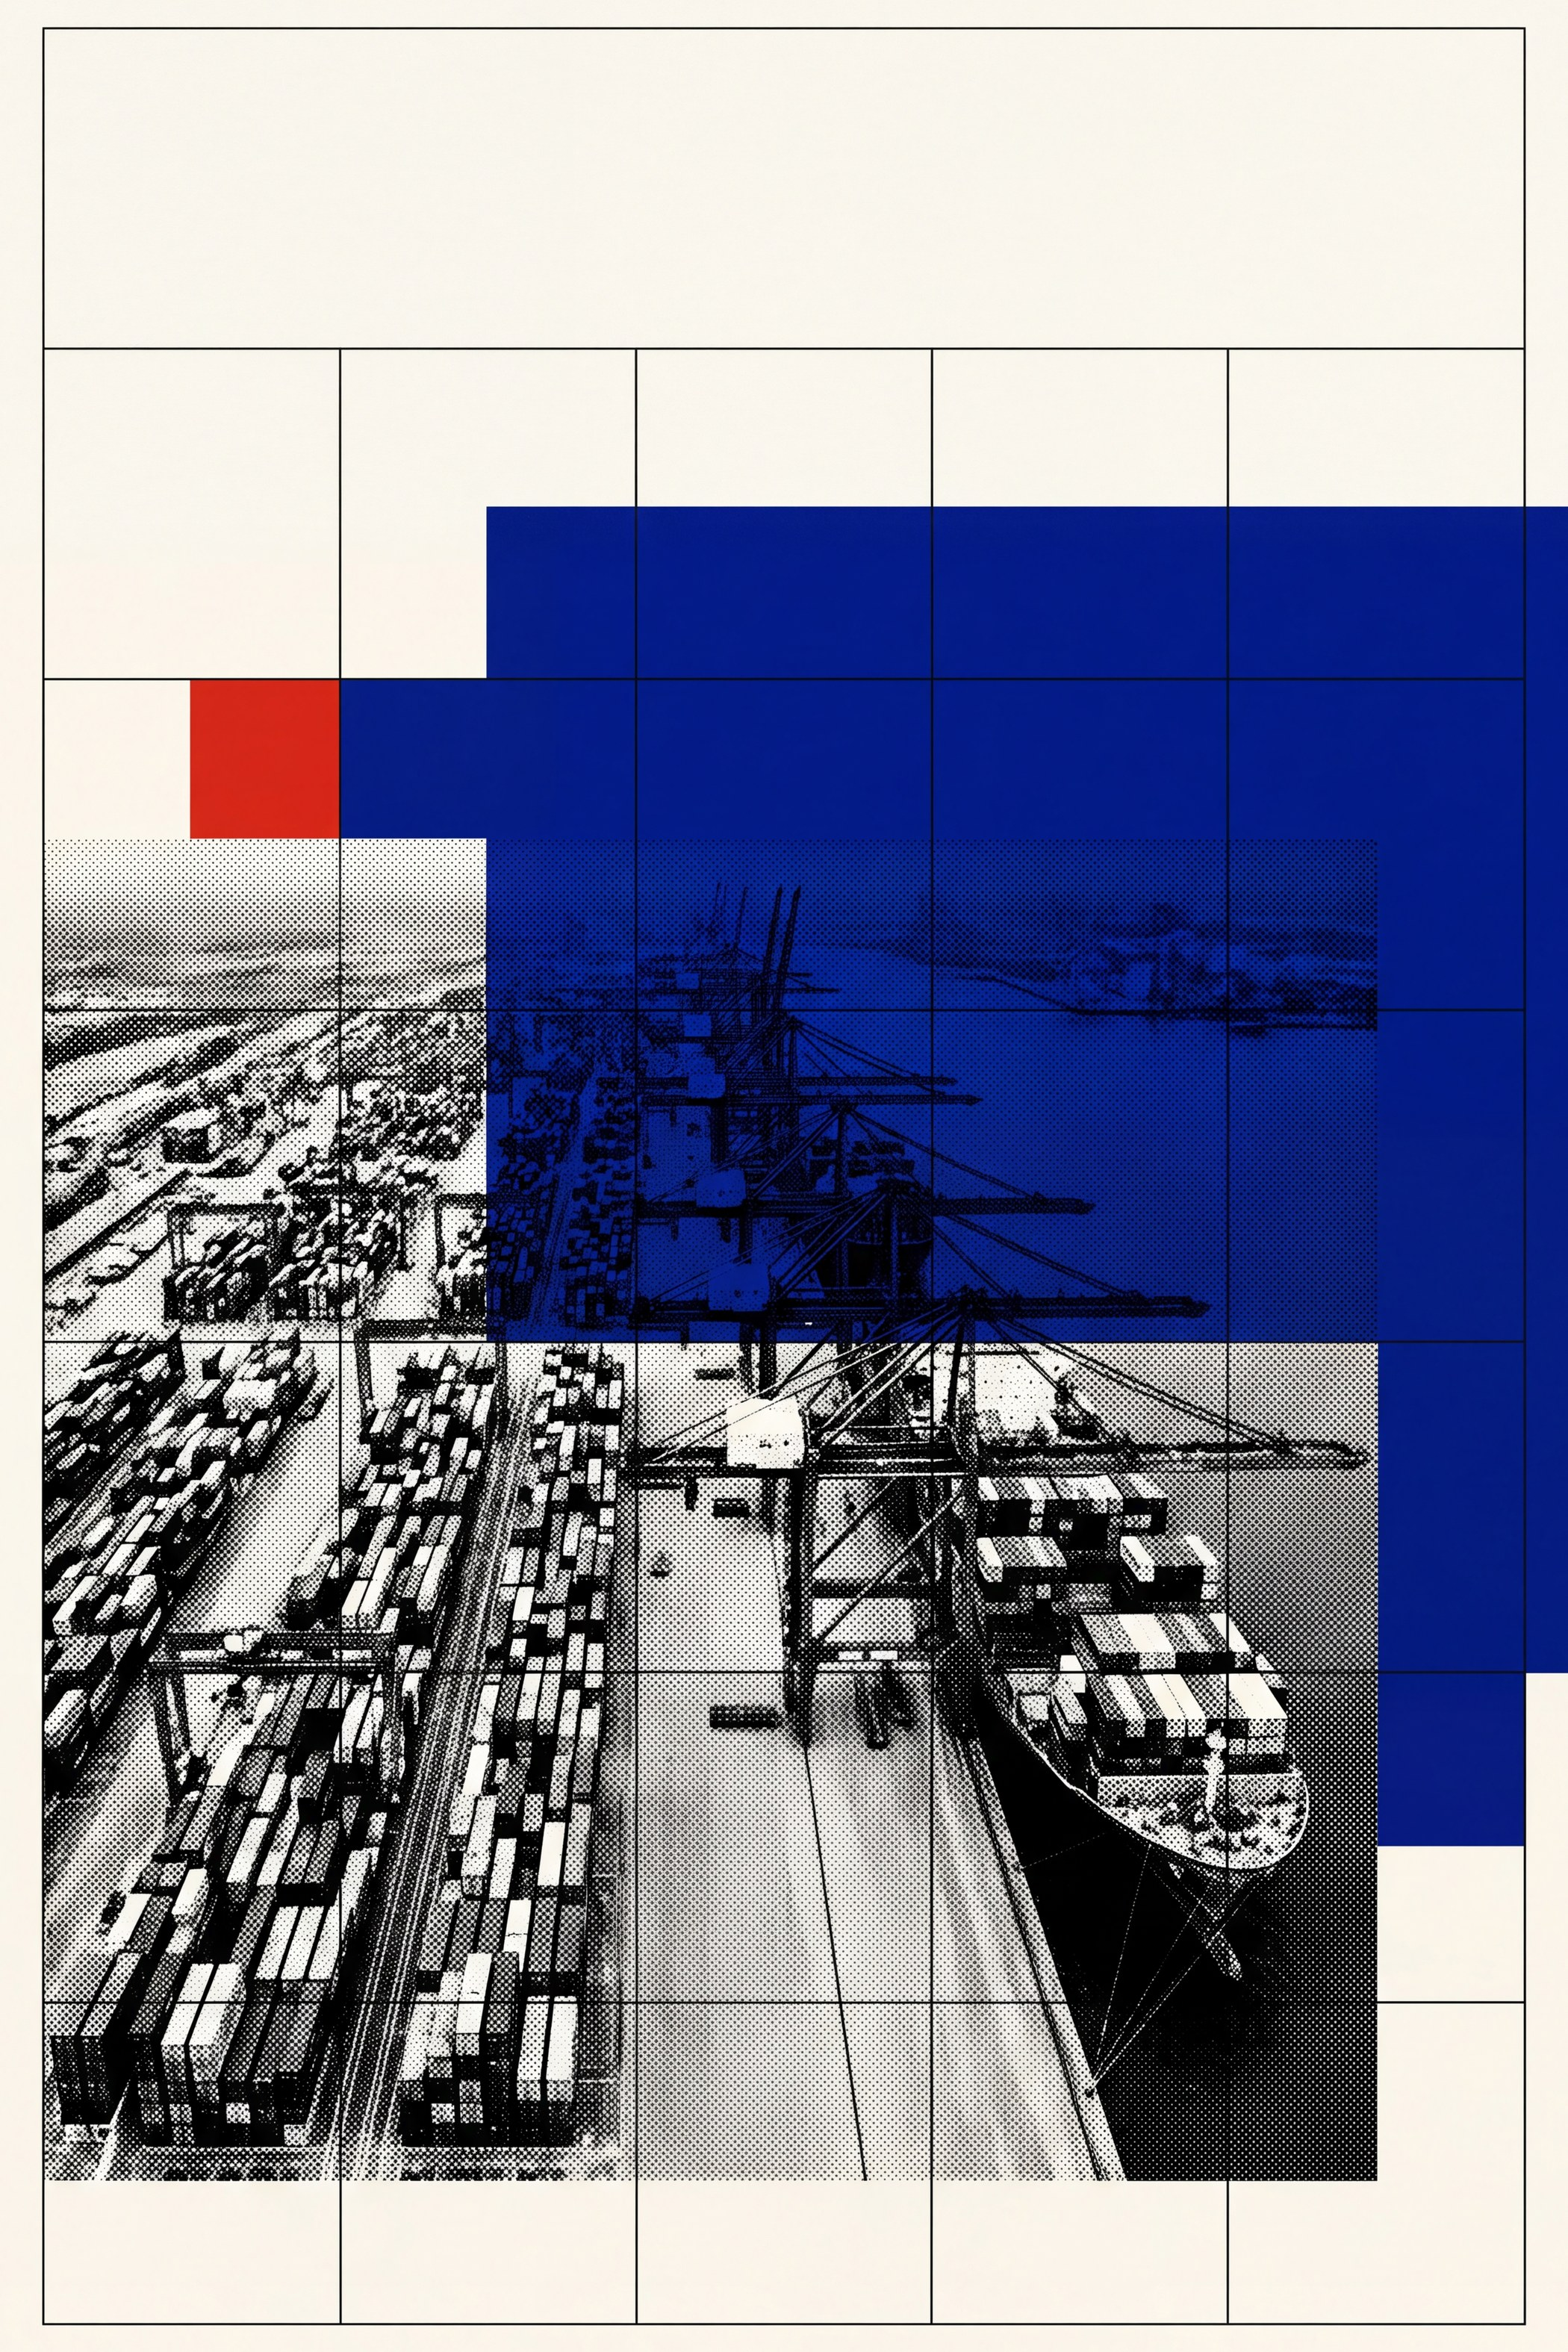
\includegraphics[width=\paperwidth,height=\paperheight]{plates/swiss/cover.jpg}}}}{%
    \PackageError{pd-swiss-plates}{Missing plate render plates/swiss/cover.jpg}{Generate the Swiss cover render and place it at plates/swiss/cover.jpg before building.}}}
\newcommand{\pdswisspartplate}[2]{% #1 numeral I..IV, #2 width
  \IfFileExists{plates/swiss/part-#1.jpg}{%
    \includegraphics[width=#2]{plates/swiss/part-#1.jpg}}{%
    \PackageError{pd-swiss-plates}{Missing plate render plates/swiss/part-#1.jpg}{Generate the Swiss part plate render and place it at plates/swiss/part-#1.jpg before building.}}}
\newcommand{\pdswissplate}[2]{% #1 chapter prefix, #2 width
  \IfFileExists{plates/swiss/chapter-#1.jpg}{%
    \includegraphics[width=#2]{plates/swiss/chapter-#1.jpg}%
  }{%
    \ifstrequal{#1}{prereq}{%
      \IfFileExists{plates/swiss/landmark-01.jpg}{%
        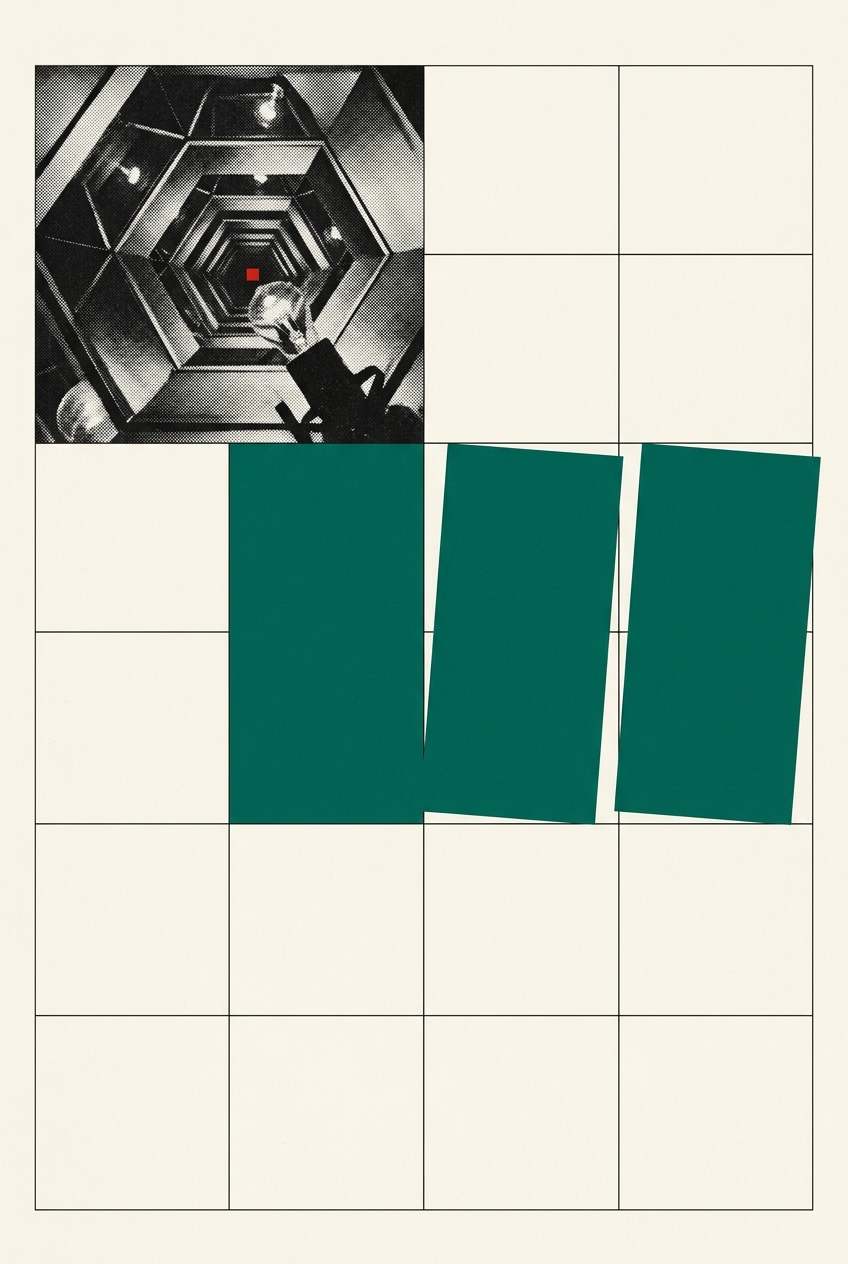
\includegraphics[width=#2]{plates/swiss/landmark-01.jpg}%
      }{%
        \PackageError{pd-swiss-plates}{Missing plate render plates/swiss/landmark-01.jpg}{Generate the Swiss landmark 01 render and place it at plates/swiss/landmark-01.jpg before building.}%
      }%
    }{%
      \PackageError{pd-swiss-plates}{Missing plate render plates/swiss/chapter-#1.jpg}{Generate the Swiss chapter plate render and place it at plates/swiss/chapter-#1.jpg before building.}%
    }%
  }%
}
\providecolor{pdswissred}{HTML}{DA291C}
\providecolor{pdcobalt}{HTML}{001489}
\providecolor{hhink}{HTML}{1B1712}
\providecolor{hhgray}{HTML}{5C5650}

% Canonical Landmark titles and pull-quotes
\expandafter\def\csname pdlandmarktitle@01\endcsname{Agentic Psychosis \& Hallucination Cascade}
\expandafter\def\csname pdlandmarkconcept@01\endcsname{Belief Drift \& Hallucination Cascades}
\expandafter\def\csname pdlandmarkquestion@01\endcsname{Can an unanchored swarm deliberate without spiraling into shared delusion?}
\expandafter\def\csname pdlandmarkquote@01\endcsname{When an unanchored swarm feeds on its own unverified assertions, error does not dissipate; it cascades into conviction. Coordination requires shared physical truth, not mutual agreement on hallucinated state.}

\expandafter\def\csname pdlandmarktitle@02\endcsname{Agentic Continuity \& The Overlapping Strand}
\expandafter\def\csname pdlandmarkconcept@02\endcsname{Substrate Continuity \& Overlapping Strands}
\expandafter\def\csname pdlandmarkquestion@02\endcsname{When every token and worker dies, what actually holds identity across time?}
\expandafter\def\csname pdlandmarkquote@02\endcsname{Identity is not an indivisible core preserved across time, but the continuous overlap of many short fibers. No single thread runs the full length of the rope; the strength is entirely in the friction between the splices.}

\expandafter\def\csname pdlandmarktitle@03\endcsname{The Engine Swap}
\expandafter\def\csname pdlandmarkconcept@03\endcsname{The Engine Swap \& Model Portability}
\expandafter\def\csname pdlandmarkquestion@03\endcsname{Can you replace the brain of a running system while keeping all its commitments intact?}
\expandafter\def\csname pdlandmarkquote@03\endcsname{The intelligence engine may be unbolted and swapped out in mid-voyage. What survives the swap is not the neural weights, but the unbroken hull of contracts, claims, and verified ledger obligations.}

\expandafter\def\csname pdlandmarktitle@04\endcsname{The Front-Loaded Probation Cliff}
\expandafter\def\csname pdlandmarkconcept@04\endcsname{The Front-Loaded Probation Cliff}
\expandafter\def\csname pdlandmarkquestion@04\endcsname{Why should an operating system ever trust an unverified autonomous actor?}
\expandafter\def\csname pdlandmarkquote@04\endcsname{Autonomy is never granted on faith; it is won against a sheer cliff of probation. The newcomer faces strict confinement until its attestation record proves it will not compromise the commons.}

\expandafter\def\csname pdlandmarktitle@05\endcsname{The Single-Writer Monotonic Horizon}
\expandafter\def\csname pdlandmarkconcept@05\endcsname{The Single-Writer Monotonic Horizon}
\expandafter\def\csname pdlandmarkquestion@05\endcsname{How do distributed agents agree on what happened first without Byzantine consensus?}
\expandafter\def\csname pdlandmarkquote@05\endcsname{One writer, one lock, one monotonic frontier. Beyond the commit horizon, the unwritten future remains empty paper; behind it, no write may ever be undone, denied, or reordered.}

\expandafter\def\csname pdlandmarktitle@06\endcsname{The Attenuation Frontier \& Cryptographic Macaroons}
\expandafter\def\csname pdlandmarkconcept@06\endcsname{The Attenuation Frontier \& Macaroons}
\expandafter\def\csname pdlandmarkquestion@06\endcsname{How do permissions travel across machines without accidentally widening?}
\expandafter\def\csname pdlandmarkquote@06\endcsname{Every delegation narrows the aperture of authority. A bearer credential cannot expand its reach as it traverses the network; it can only accumulate cryptographic caveats that bind its hands.}

\expandafter\def\csname pdlandmarktitle@07\endcsname{Attestation Without Revelation (The Sealed Harbor)}
\expandafter\def\csname pdlandmarkconcept@07\endcsname{Attestation Without Revelation (Sealed Harbor)}
\expandafter\def\csname pdlandmarkquestion@07\endcsname{Can a worker prove its computation was correct without revealing what it saw?}
\expandafter\def\csname pdlandmarkquote@07\endcsname{The enclave proves what was computed without disclosing what was seen. Trust in autonomous labor cannot demand total transparency; it demands unforgeable evidence of compliance.}

\expandafter\def\csname pdlandmarktitle@08\endcsname{Read-Poverty \& The Legible Swarm}
\expandafter\def\csname pdlandmarkconcept@08\endcsname{Read-Poverty \& Stigmergic Signaling}
\expandafter\def\csname pdlandmarkquestion@08\endcsname{Why is an agent that reads everything destined to bankrupt its operator?}
\expandafter\def\csname pdlandmarkquote@08\endcsname{In an ocean of synthetic prose, reading is infinitely more expensive than writing. A legible swarm does not shout across channels; it leaves quiet, structured pheromones in the environment.}

\expandafter\def\csname pdlandmarktitle@09\endcsname{Skills as Capital vs.\ Token Labor}
\expandafter\def\csname pdlandmarkconcept@09\endcsname{Skills as Capital vs. Perishable Token Labor}
\expandafter\def\csname pdlandmarkquestion@09\endcsname{When does prompt deliberation become too expensive compared to compiled code?}
\expandafter\def\csname pdlandmarkquote@09\endcsname{Token generation is perishable labor; compiled deterministic tools are durable capital. An economy matures when agents stop paying per token to deliberate and start amortizing proven apparatus.}

\expandafter\def\csname pdlandmarktitle@10\endcsname{The Bonded Commons \& Sacrificial Slashing}
\expandafter\def\csname pdlandmarkconcept@10\endcsname{The Bonded Commons \& Sacrificial Slashing}
\expandafter\def\csname pdlandmarkquestion@10\endcsname{What stops an agent from promising the world and walking away from disaster?}
\expandafter\def\csname pdlandmarkquote@10\endcsname{Trust without collateral is wishful thinking. An agent stakes its bond in the escrow of the commons; when an invariant is breached, the tripwire snaps and the stake is forfeited without appeal.}

\expandafter\def\csname pdlandmarktitle@11\endcsname{Sheaf Laplacian Invariance \& Cycle Consistency}
\expandafter\def\csname pdlandmarkconcept@11\endcsname{Sheaf Laplacians \& Cycle Holonomy}
\expandafter\def\csname pdlandmarkquestion@11\endcsname{Can a network of liars agree locally on every edge while still being caught globally?}
\expandafter\def\csname pdlandmarkquote@11\endcsname{Local consistency along every pairwise edge does not guarantee global truth. When an assertion traverses a closed cycle of harbors and returns altered, the non-zero holonomy reveals the fraud.}

\expandafter\def\csname pdlandmarktitle@12\endcsname{The Zombie Reclaim \& Salvage Graveyard}
\expandafter\def\csname pdlandmarkconcept@12\endcsname{Zombie Salvage \& Dead-Man Leases}
\expandafter\def\csname pdlandmarkquestion@12\endcsname{When an agent crashes in the dark, who buries the body and recovers the locks?}
\expandafter\def\csname pdlandmarkquote@12\endcsname{The graveyard of abandoned sessions is the foundation of harbor resilience. When a heartbeat goes cold, no ghost may linger; the lease expires, the locks are salvaged, and the port is reclaimed.}

% Single-digit alias fallbacks
\expandafter\def\csname pdlandmarktitle@1\endcsname{\csname pdlandmarktitle@01\endcsname}
\expandafter\def\csname pdlandmarkconcept@1\endcsname{\csname pdlandmarkconcept@01\endcsname}
\expandafter\def\csname pdlandmarkquestion@1\endcsname{\csname pdlandmarkquestion@01\endcsname}
\expandafter\def\csname pdlandmarkquote@1\endcsname{\csname pdlandmarkquote@01\endcsname}

\expandafter\def\csname pdlandmarktitle@2\endcsname{\csname pdlandmarktitle@02\endcsname}
\expandafter\def\csname pdlandmarkconcept@2\endcsname{\csname pdlandmarkconcept@02\endcsname}
\expandafter\def\csname pdlandmarkquestion@2\endcsname{\csname pdlandmarkquestion@02\endcsname}
\expandafter\def\csname pdlandmarkquote@2\endcsname{\csname pdlandmarkquote@02\endcsname}

\expandafter\def\csname pdlandmarktitle@3\endcsname{\csname pdlandmarktitle@03\endcsname}
\expandafter\def\csname pdlandmarkconcept@3\endcsname{\csname pdlandmarkconcept@03\endcsname}
\expandafter\def\csname pdlandmarkquestion@3\endcsname{\csname pdlandmarkquestion@03\endcsname}
\expandafter\def\csname pdlandmarkquote@3\endcsname{\csname pdlandmarkquote@03\endcsname}

\expandafter\def\csname pdlandmarktitle@4\endcsname{\csname pdlandmarktitle@04\endcsname}
\expandafter\def\csname pdlandmarkconcept@4\endcsname{\csname pdlandmarkconcept@04\endcsname}
\expandafter\def\csname pdlandmarkquestion@4\endcsname{\csname pdlandmarkquestion@04\endcsname}
\expandafter\def\csname pdlandmarkquote@4\endcsname{\csname pdlandmarkquote@04\endcsname}

\expandafter\def\csname pdlandmarktitle@5\endcsname{\csname pdlandmarktitle@05\endcsname}
\expandafter\def\csname pdlandmarkconcept@5\endcsname{\csname pdlandmarkconcept@05\endcsname}
\expandafter\def\csname pdlandmarkquestion@5\endcsname{\csname pdlandmarkquestion@05\endcsname}
\expandafter\def\csname pdlandmarkquote@5\endcsname{\csname pdlandmarkquote@05\endcsname}

\expandafter\def\csname pdlandmarktitle@6\endcsname{\csname pdlandmarktitle@06\endcsname}
\expandafter\def\csname pdlandmarkconcept@6\endcsname{\csname pdlandmarkconcept@06\endcsname}
\expandafter\def\csname pdlandmarkquestion@6\endcsname{\csname pdlandmarkquestion@06\endcsname}
\expandafter\def\csname pdlandmarkquote@6\endcsname{\csname pdlandmarkquote@06\endcsname}

\expandafter\def\csname pdlandmarktitle@7\endcsname{\csname pdlandmarktitle@07\endcsname}
\expandafter\def\csname pdlandmarkconcept@7\endcsname{\csname pdlandmarkconcept@07\endcsname}
\expandafter\def\csname pdlandmarkquestion@7\endcsname{\csname pdlandmarkquestion@07\endcsname}
\expandafter\def\csname pdlandmarkquote@7\endcsname{\csname pdlandmarkquote@07\endcsname}

\expandafter\def\csname pdlandmarktitle@8\endcsname{\csname pdlandmarktitle@08\endcsname}
\expandafter\def\csname pdlandmarkconcept@8\endcsname{\csname pdlandmarkconcept@08\endcsname}
\expandafter\def\csname pdlandmarkquestion@8\endcsname{\csname pdlandmarkquestion@08\endcsname}
\expandafter\def\csname pdlandmarkquote@8\endcsname{\csname pdlandmarkquote@08\endcsname}

\expandafter\def\csname pdlandmarktitle@9\endcsname{\csname pdlandmarktitle@09\endcsname}
\expandafter\def\csname pdlandmarkconcept@9\endcsname{\csname pdlandmarkconcept@09\endcsname}
\expandafter\def\csname pdlandmarkquestion@9\endcsname{\csname pdlandmarkquestion@09\endcsname}
\expandafter\def\csname pdlandmarkquote@9\endcsname{\csname pdlandmarkquote@09\endcsname}

\newcommand{\pdlandmarktocentry}[2]{%
  \par\addvspace{5pt}\noindent
  \begin{tikzpicture}
    % Background card
    \draw[draw=pdcobalt!25,fill=pdcobalt!2,rounded corners=2pt,line width=0.5pt] (0,0) rectangle (\linewidth, 1.25in);
    \fill[pdcobalt] (0,0) rectangle (3pt, 1.25in);
    
    % Text container
    \node[anchor=north west,inner sep=0pt,text width=0.60\linewidth] at (8pt, 1.25in-6pt) {%
      {\fontsize{8}{10}\selectfont\color{pdcobalt}\bfseries
        Landmark #1\enspace\textperiodcentered\enspace#2}\par\vspace{3pt}%
      \ifcsname pdlandmarkconcept@#1\endcsname
        \colorbox{pdcobalt!10}{\fontsize{6.2}{7.5}\selectfont\bfseries\color{pdcobalt}Governing Concept: \csname pdlandmarkconcept@#1\endcsname}\par\vspace{3pt}%
      \fi
      \ifcsname pdlandmarkquestion@#1\endcsname
        {\fontsize{6}{7.6}\selectfont\itshape\color{hhink}``\csname pdlandmarkquestion@#1\endcsname''}\par\vspace{4pt}%
      \fi
      \tikz[baseline=-2pt]{\draw[draw=pdcobalt,line width=0.9pt,-{Stealth[length=4pt,width=3pt]}] (0,0.08) -- (0.7,0.08) |- (1.5,-0.04);}%
      \enspace{\fontsize{6}{7.2}\selectfont\bfseries\color{pdcobalt}See Plate on page \ifdefined\pdcurrentplatepage\pdcurrentplatepage\fi}%
    };
    
    % Framed thumbnail image on the right
    \node[anchor=north east,inner sep=0pt] at (\linewidth-6pt, 1.25in-6pt) {%
      \fcolorbox{pdcobalt!35}{white}{%
        \includegraphics[width=0.34\linewidth,height=1.13in,keepaspectratio]{plates/swiss/landmark-#1.jpg}%
      }%
    };
  \end{tikzpicture}\par\addvspace{5pt}%
}

\newcommand{\pdswisslandmarkplate}[2]{% #1 landmark ID (e.g. 01..12), #2 width
  \IfFileExists{plates/swiss/landmark-#1.jpg}{%
    \phantomsection\label{landmark:#1}%
    \addcontentsline{toc}{pdplate}{\protect\texorpdfstring{\protect\pdlandmarktocentry{#1}{\csname pdlandmarktitle@#1\endcsname}}{Landmark #1: \csname pdlandmarktitle@#1\endcsname}}%
    \centering
    \includegraphics[width=#2]{plates/swiss/landmark-#1.jpg}%
    \par\vspace{10pt}%
    \begin{minipage}{\linewidth}%
      {\color{pdcobalt}\rule{\linewidth}{1.2pt}}\par\vspace{6pt}%
      \raggedright
      {\color{pdswissred}\rule{4.5pt}{4.5pt}}\enspace%
      {\pdgrotesk\bfseries\scshape\fontsize{9}{11}\selectfont\color{hhink}%
        Landmark #1\enspace\textperiodcentered\enspace\csname pdlandmarktitle@#1\endcsname}\par\vspace{4.5pt}%
      {\pdgrotesk\itshape\fontsize{9.5}{13.5}\selectfont\color{hhink}%
        ``\csname pdlandmarkquote@#1\endcsname''\par}%
      \vspace{6pt}%
      {\color{hhgray!30}\rule{\linewidth}{0.4pt}}%
    \end{minipage}%
  }{%
    \PackageError{pd-swiss-plates}{Missing plate render plates/swiss/landmark-#1.jpg}{Generate the Swiss landmark plate render and place it at plates/swiss/landmark-#1.jpg before building.}}}
\makeatother

\fi

% The maturity, guarantee, proof-obligation and claim-evidence vocabularies --
% \Built, \BuiltWeak, \Designed, \Vision, their uppercase aliases, \NotGuar,
% \Closed, \Partial, \Open, \SpecOnly, \Verified, \Proved, \Unproved -- and
% \code are defined once, for this volume and for every standalone chapter, in
% figures/pd-pedagogy.tex (\input above).
%
% They used to be listed here AND again in each chapter's own preamble. The
% generator keeps only what lies between \begin{document} and \end{document},
% so the chapter copies never reached this document and the two sets were free
% to disagree -- which they did: chapter 4 printed "built" and "designed" when
% it compiled alone and "implemented" and "specified" at the same call sites
% here. One definition, in a file both preambles read, is what makes a marker
% mean the same thing in both places.
% scripts/harbor-research/check_duplicate_macros.py fails the build if a
% second definition of any of these names comes back.

\newcommand{\pullquote}[1]{%
  \par\vspace{6pt}\noindent\begin{tikzpicture}
  \node[draw=none,fill=hhsand!22,inner sep=10pt,text width=\dimexpr\textwidth-30pt\relax,align=left] (q) {\itshape\large #1};
  \draw[hhcobalt,line width=2.5pt] (q.north west) -- (q.south west);
  \end{tikzpicture}\par\vspace{6pt}}
\newcommand{\keyidea}[1]{%
  \par\vspace{6pt}\noindent\begin{tikzpicture}
  \node[draw=none,fill=hhsand!18,rounded corners=2pt,inner sep=9pt,text width=\dimexpr\textwidth-26pt\relax,align=left] (k)
        {{\scshape\bfseries\color{hhgray}\small Key idea.}\enspace #1};
  \draw[hhgray!60,line width=1pt] (k.north west) -- (k.south west);
  \end{tikzpicture}\par\vspace{6pt}}
\newcommand{\pitfall}[1]{%
  \par\vspace{6pt}\noindent\begin{tikzpicture}
  \node[draw=none,fill=hhsand!18,rounded corners=2pt,inner sep=9pt,text width=\dimexpr\textwidth-26pt\relax,align=left] (p)
        {{\scshape\bfseries\color{hhcobalt}\small Pitfall.}\enspace #1};
  \draw[hhgray!60,line width=1pt] (p.north west) -- (p.south west);
  \end{tikzpicture}\par\vspace{6pt}}
\newcommand{\xrefbox}[1]{%
  \vspace{4pt}\noindent\begin{tikzpicture}
  \node[draw=hhgray!45,line width=0.4pt,fill=hhsand!18,rounded corners=2pt,inner sep=8pt,text width=\dimexpr\textwidth-22pt\relax,align=left]{\small #1};
  \end{tikzpicture}\vspace{4pt}}
\newcommand{\scene}[2]{%
  \par\vspace{6pt}\noindent\begin{tikzpicture}
  \node[draw=none,fill=hhsand!18,rounded corners=2pt,inner sep=9pt,text width=\dimexpr\textwidth-28pt\relax,align=left] (s)
        {{\scshape\bfseries\color{hhgray}\footnotesize Scene.}\enspace{\bfseries #1}\enspace\itshape #2};
  \draw[hhgray!60,line width=1pt] (s.north west) -- (s.south west);
  \end{tikzpicture}\par\vspace{6pt}}
\newcommand{\openstar}{{\textcolor{hhcobalt}{$\bigstar$}}\;}
\newcommand{\exhead}[1]{\par\vspace{4pt}\noindent{\scshape\bfseries\color{hhink}#1}\par\vspace{-2pt}}

% Chapter-local exercise idioms keep authored semantics under one visual grammar.
\newenvironment{lsexercises}{%
  \par\vspace{8pt}\noindent\begin{tikzpicture}
  \node[draw=hhgray!45,line width=0.4pt,fill=hhsand!12,rounded corners=2pt,inner sep=10pt,text width=\dimexpr\textwidth-28pt\relax,align=left]\bgroup
  \begin{minipage}{\dimexpr\textwidth-30pt\relax}
  {\scshape\bfseries\color{hhink}Exercises}\par\vspace{3pt}\small
}{\end{minipage}\egroup;\end{tikzpicture}\par\vspace{8pt}}
\newenvironment{stpexercises}{%
  \par\vspace{8pt}\noindent\begin{tikzpicture}
  \node[draw=hhgray!45,line width=0.4pt,fill=hhsand!12,rounded corners=2pt,inner sep=10pt,text width=\dimexpr\textwidth-26pt\relax,align=left]\bgroup
  \begin{minipage}{\dimexpr\textwidth-46pt\relax}
  {\scshape\bfseries\color{hhink}\large Exercises}\par\vspace{3pt}\small
}{\end{minipage}\egroup;\end{tikzpicture}\par\vspace{8pt}}
\newenvironment{heexercises}{%
  \par\vspace{8pt}\noindent
  {\scshape\bfseries\textcolor{hhink}{\textcolor{hhgray!70}{\rule[-1pt]{2.5pt}{11pt}}\enspace Exercises}}
  \par\nobreak\vspace{2pt}
  \begin{enumerate}[label=\textbf{E\arabic*.},leftmargin=2.6em,itemsep=2pt,topsep=2pt]
}{\end{enumerate}\vspace{6pt}}
\newcommand{\swkexercises}[1]{%
  \par\vspace{8pt}\noindent\begin{tikzpicture}
  \node[draw=hhgray!45,line width=0.4pt,fill=hhsand!12,rounded corners=2pt,inner sep=9pt,text width=\dimexpr\textwidth-26pt\relax,align=left]
        {{\scshape\bfseries\textcolor{hhink}{Exercises.}}\par\vspace{3pt}#1};
  \end{tikzpicture}\par\vspace{6pt}}

% Code and pseudocode as a printed book sets them: an indented block in a
% dense monospace with tight leading, keywords bold, comments italic grey,
% small grey line numbers, no frame, no background, no stripes. A wrapped
% line continues under a small grey hook.
\lstdefinestyle{pdcode}{language=C,backgroundcolor={},frame=none,
  basicstyle=\ttfamily\fontsize{8.6}{10.6}\selectfont,columns=fullflexible,keepspaces=true,
  keywordstyle=\bfseries,commentstyle=\color{hhgray}\itshape,
  stringstyle=\color{hhink!70!hhgray},numbers=left,numberstyle=\fontsize{6.5}{7}\selectfont\color{hhgray},
  numbersep=7pt,breaklines=true,breakatwhitespace=false,breakindent=1.6em,
  postbreak=\mbox{\textcolor{hhgray}{\fontsize{7}{7}\selectfont$\hookrightarrow$}\space},
  showstringspaces=false,tabsize=2,aboveskip=7pt,belowskip=5pt,
  xleftmargin=1.9em,xrightmargin=0pt,captionpos=b}
\lstdefinestyle{pseudocode}{style=pdcode,
  morekeywords={function,return,if,then,else,for,while,do,begin,end,atomic,transaction,reject,commit,assert,raise}}
\lstdefinestyle{proverif}{style=pdcode}
\lstdefinestyle{rust}{style=pdcode,tabsize=4}
\lstdefinestyle{tlaplus}{style=pdcode,
  morekeywords={MODULE,EXTENDS,CONSTANTS,VARIABLES,VARIABLE,Init,Next,Spec,
  TypeOK,IF,THEN,ELSE,LET,IN,CHOOSE,SUBSET,UNION,DOMAIN,EXCEPT,
  UNCHANGED,TRUE,FALSE,BOOLEAN,Nat,Int,STRING,Seq,Append,Len,Head,Tail,
  ENABLED,WF_,SF_,THEOREM,ASSUME,INSTANCE,WITH,LOCAL}}
\lstset{style=pdcode}

\theoremstyle{definition}
\newtheorem{definition}{Definition}[section]
\newtheorem{property}{Property}[section]
\newtheorem{protocol}{Protocol}[section]
\theoremstyle{plain}
\newtheorem{theorem}{Theorem}[section]
\newtheorem{lemma}{Lemma}[section]
\newtheorem{proposition}{Proposition}[section]
\newtheorem{corollary}{Corollary}[section]
\newtheorem{conjecture}{Conjecture}[section]
\theoremstyle{remark}
\newtheorem*{remark}{Remark}

\newcounter{lsprotocol}[section]
\renewcommand{\thelsprotocol}{\thesection.\arabic{lsprotocol}}
\newenvironment{lsprotocol}[1]{%
  \par\vspace{8pt}\refstepcounter{lsprotocol}\noindent\begin{tikzpicture}
  \node[draw=hhgray!45,line width=0.4pt,fill=hhsand!12,rounded corners=2pt,inner sep=10pt,text width=\dimexpr\textwidth-28pt\relax,align=left]\bgroup
  \begin{minipage}{\dimexpr\textwidth-30pt\relax}
  {\scshape\bfseries\color{hhink}Protocol~\thelsprotocol.}\enspace{\bfseries #1}\par\vspace{4pt}\small
}{\end{minipage}\egroup;\end{tikzpicture}\par\vspace{8pt}}
\newcounter{stpprotocol}[section]
\renewcommand{\thestpprotocol}{\thesection.\arabic{stpprotocol}}
\newenvironment{stpprotocol}[1][]{%
  \par\vspace{8pt}\refstepcounter{stpprotocol}\noindent\begin{tikzpicture}
  \node[draw=hhgray!45,line width=0.4pt,fill=hhsand!12,rounded corners=2pt,inner sep=10pt,text width=\dimexpr\textwidth-26pt\relax,align=left]\bgroup
  \begin{minipage}{\dimexpr\textwidth-46pt\relax}
  {\scshape\bfseries\color{hhink}Protocol~\thestpprotocol.}%
  \ifx\\#1\\\else\ {\bfseries #1}\fi\par\vspace{3pt}\small
}{\end{minipage}\egroup;\end{tikzpicture}\par\vspace{8pt}}
\theoremstyle{definition}
\newtheorem{heprotocol}{Protocol}[section]

\tikzset{
  stp box/.style={draw=hhink,line width=0.55pt,fill=hhsand!22,rounded corners=2pt,inner sep=7pt,align=center,minimum height=10mm},
  stp accent box/.style={stp box,draw=hhcobalt,line width=0.9pt},
  stp arrow/.style={-{Stealth[length=2.3mm,width=1.5mm]},draw=hhink,line width=0.65pt},
  stp accent arrow/.style={-{Stealth[length=2.3mm,width=1.5mm]},draw=hhcobalt,line width=0.8pt},
  stp dashed arrow/.style={stp accent arrow,dashed},
  stp label/.style={fill=hhpaper,inner xsep=3pt,inner ysep=1.5pt,font=\footnotesize\itshape,text=hhgray},
  stp heading/.style={font=\footnotesize\bfseries,text=hhink},
  stp status/.style={font=\scriptsize\scshape,text=hhgray},
}

\pagestyle{fancy}
\fancyhf{}
\fancyhead[L]{\small\itshape\color{hhgray} \pdeditiontitle}
\fancyhead[R]{\small\color{hhgray}\thepage}
\fancyfoot[C]{\footnotesize\color{hhgray} Textbook Edition \textperiodcentered\ \pdeditiondate}
\renewcommand{\headrulewidth}{0.4pt}
\renewcommand{\footrulewidth}{0pt}

% ---- Chapters, parts, and the front-matter map ----------------------------
% Chapter numbers are Arabic and come from whitepaper/textbook.json via the
% generator: \pdchapter{number}{title}{prefix}{hue}. The prefix selects the
% chapter's seam rails and its entry in figures/pd-textbook-map.tex (question,
% epigraph, one-breath answer, part label); the hue is the PART's, inherited by
% every chapter in it, so each part owns one color and nothing dilutes it.
\newcounter{pdchapter}
\renewcommand{\thepdchapter}{\arabic{pdchapter}}
\makeatletter
\@namedef{theHpdchapter}{chap.\arabic{pdchapter}}
\makeatother
\newcommand{\pdcurrentchapter}{0}
\newcommand{\pdcurrentchaptercolor}{pdcobalt}
% A live link to a chapter, by prefix. figures/pd-hyperlinks.tex provides the
% plain-text fallback for standalone chapters; the Book defines the real thing.
\DeclareRobustCommand{\pdchaplink}[2]{\hyperref[chap:#1]{#2}}

% The weighted four-hue rule. One segment per part, its length proportional to
% the part's share of the book's pages (from the page references once they
% exist; chapter counts on the first pass). Segments up to the current part are
% solid, the rest outlined, so the same rule reads as a progress mark on part
% and chapter openers and as the whole book on the title page.
%   \pdweightrule[color]{current part index or 0 for all}{total width}{height}
\newdimen\pdweightx
\newdimen\pdweightw
\newcount\pdweighti
\makeatletter
\newcommand{\pdweightrule}[4][]{%
  \begingroup
  \edef\pd@tot{\the\numexpr\getpagerefnumber{book:appendices}-\getpagerefnumber{part:\pdfirstpartnumeral}\relax}%
  \ifnum\pd@tot<1 \def\pd@tot{0}\fi
  \pdweightx=0pt \pdweighti=0
  \def\pdweightsegment##1##2##3##4{%
    \advance\pdweighti by 1
    \ifnum\pd@tot>0
      \edef\pd@seg{\the\numexpr\getpagerefnumber{##3}-\getpagerefnumber{part:##1}\relax}%
      \ifnum\pd@seg<1 \edef\pd@seg{##4}\edef\pd@den{\pdchaptercount}\else\edef\pd@den{\pd@tot}\fi
    \else
      \edef\pd@seg{##4}\edef\pd@den{\pdchaptercount}%
    \fi
    \pdweightw=\dimexpr(#3-3pt*(\pdpartcount-1))*\pd@seg/\pd@den\relax
    \if\relax\detokenize{#1}\relax\def\pd@col{##2}\else\def\pd@col{#1}\fi
    \ifnum#2=0 \def\pd@solid{1}\else\ifnum\pdweighti>#2 \def\pd@solid{0}\else\def\pd@solid{1}\fi\fi
    \if1\pd@solid
      \fill[color=\pd@col] (\the\pdweightx,0pt) rectangle ++(\the\pdweightw,#4);
    \else
      \draw[color=\pd@col,line width=0.5pt] (\the\dimexpr\pdweightx+0.25pt\relax,0.25pt) rectangle ++(\the\dimexpr\pdweightw-0.5pt\relax,\the\dimexpr#4-0.5pt\relax);
    \fi
    \advance\pdweightx by \pdweightw \advance\pdweightx by 3pt
  }%
  \begin{tikzpicture}[baseline=0pt]
    \pdweightsegmentslist
  \end{tikzpicture}%
  \endgroup}
\makeatother

% The chapter opener: one page with the title, an epigraph, a plate when the
% chapter has one, and the question the chapter answers with its one-breath
% answer. Nothing else. The chapter's first section starts on the next page.
\makeatletter
\def\pd@chapter@maritime#1#2#3#4{%
  \vspace*{0.1cm}
  \noindent{\scshape\footnotesize\color{hhgray}Chapter #1 of \pdchaptercount\hfill\pdchapterpartlabel}\par
  \vspace{0.25cm}
  \noindent\pdweightrule{\pdchapterpartindex}{\textwidth}{2pt}\par
  % The gilt fillet: the trim line of the engraved plates, carried onto the
  % page. Hairline, under the weight rule, and nowhere else on the spread.
  \vspace{2.6pt}\noindent{\color{pdmaritimegold}\rule{\textwidth}{0.4pt}}\par
  \vspace{\dimexpr1.3cm-3pt\relax}
  {\noindent\fontsize{34}{40}\selectfont\color{hhink}\hyphenpenalty=10000\exhyphenpenalty=10000\raggedright #2\par}
  \vspace{1.0cm}
  \begin{flushright}
    \begin{minipage}{0.84\textwidth}\raggedleft
      {\itshape\pdchapterepigraph\par}
      \vspace{5pt}
      {\footnotesize\scshape\color{hhgray}\pdchapterepigraphsource\par}
    \end{minipage}
  \end{flushright}
  % The question block is measured first, then the plate takes what the page
  % still has above it (capped at 0.42 of the text height), and the question
  % closes the page as in the first printing. Nothing can spill: the plate is
  % cut to fit and dropped below 3 cm.
  \sbox{\pdqbox}{\begin{minipage}{\textwidth}
    \noindent{\scshape\footnotesize\color{hhgray}The question this chapter answers}\par
    \vspace{6pt}
    {\noindent\fontsize{21}{26}\selectfont\color{hhink}\hyphenpenalty=10000\exhyphenpenalty=10000\raggedright\pdchapterquestion\par}
    \vspace{9pt}
    {\noindent\small\itshape\pdchapteroneline\par}
  \end{minipage}}%
  \par
  \IfFileExists{plates/chapter-#3.jpg}{%
    \ifdim\pagegoal=\maxdimen
      \setlength{\pdplateh}{\dimexpr\textheight-\pagetotal\relax}%
    \else
      \setlength{\pdplateh}{\dimexpr\pagegoal-\pagetotal\relax}%
    \fi
    \addtolength{\pdplateh}{-\ht\pdqbox}\addtolength{\pdplateh}{-\dp\pdqbox}\addtolength{\pdplateh}{-1.6cm}%
    \ifdim\pdplateh>0.42\textheight \setlength{\pdplateh}{0.42\textheight}\fi
    \ifdim\pdplateh>3cm
      \vspace{0.5cm}%
      \noindent\makebox[\textwidth]{\includegraphics[width=\textwidth,height=\pdplateh,keepaspectratio]{plates/chapter-#3.jpg}}\par
    \fi}{}%
  \vfill
  \noindent\usebox{\pdqbox}\par
  \vspace{0.2cm}
}
% swiss: a colour band carries number and title; the question sits on paper
\def\pd@chapter@swiss#1#2#3#4{%
  \begin{adjustwidth}{0pt}{-\dimexpr\marginparsep+\marginparwidth\relax}
  \vspace*{-0.5cm}
  \noindent\begin{tikzpicture}
    \node[fill=#4,inner sep=0pt,minimum width=\linewidth,minimum height=0.36\textheight,anchor=north west] (band) at (0,0) {};
    \node[anchor=north west,text=hhpaper,font=\pdgrotesk\fontsize{9.5}{12}\selectfont\bfseries,inner sep=0pt]
      at (0.45cm,-0.5cm) {Chapter #1 of \pdchaptercount\quad\textperiodcentered\quad\pdchapterpartlabel};
    \node[anchor=south west,text=hhpaper,font=\pdgrotesk\fontsize{78}{78}\selectfont\bfseries,inner sep=0pt]
      at (0.4cm,{-0.36\textheight+3.0cm}) {#1};
    \node[anchor=south west,text=hhpaper,font=\pdgrotesk\fontsize{27}{31}\selectfont\bfseries,inner sep=0pt,
      text width={\dimexpr\linewidth-1cm\relax},align=left] at (0.45cm,{-0.36\textheight+0.55cm}) {#2};
  \end{tikzpicture}\par
  \vspace{1.0cm}
  \noindent{\pdgrotesk\footnotesize\bfseries\color{hhgray}The question this chapter answers}\par
  \vspace{6pt}
  {\noindent\fontsize{21}{26}\selectfont\color{hhink}\hyphenpenalty=10000\exhyphenpenalty=10000\raggedright\pdchapterquestion\par}
  \vspace{9pt}
  {\noindent\small\itshape\pdchapteroneline\par}
  \vspace{0.9cm}
  \noindent\pdswissplate{#3}{0.7\linewidth}\par
  \vfill
  \begin{flushright}
    \begin{minipage}{0.84\linewidth}\raggedleft
      {\itshape\pdchapterepigraph\par}
      \vspace{5pt}
      {\pdgrotesk\footnotesize\color{hhgray}\pdchapterepigraphsource\par}
    \end{minipage}
  \end{flushright}
  \vspace{0.3cm}
  \end{adjustwidth}}
% technical: a drawing sheet; the chapter numeral in the accent, the title
% block at the foot
\def\pd@chapter@technical#1#2#3#4{%
  \pd@techsheet{#2}{Chapter #1}%
  \begin{adjustwidth}{0pt}{-1.0in}
  \vspace*{0.5cm}
  \noindent{\pdgrotesk\footnotesize Chapter #1 of \pdchaptercount\hfill\pdchapterpartlabel}\par
  \vspace{0.3cm}\noindent{\color{hhink}\rule{\linewidth}{0.5pt}}\par
  \vspace{0.9cm}
  \noindent{\pdgrotesk\fontsize{60}{60}\selectfont\color{pdamber}#1\par}
  \vspace{0.2cm}
  \noindent{\pdgrotesk\fontsize{26}{31}\selectfont\hyphenpenalty=10000\exhyphenpenalty=10000\raggedright #2\par}
  \vspace{0.3cm}
  \begin{flushright}
    \begin{minipage}{0.84\linewidth}\raggedleft
      {\itshape\pdchapterepigraph\par}
      \vspace{5pt}
      {\pdgrotesk\footnotesize\color{hhgray}\pdchapterepigraphsource\par}
    \end{minipage}
  \end{flushright}
  % The question block is measured first; the plate takes what the page still
  % has above it, less the 1.6 cm the title block occupies at the sheet's foot.
  \sbox{\pdqbox}{\begin{minipage}{\linewidth}
    \noindent{\pdgrotesk\footnotesize\bfseries\color{hhgray}The question this chapter answers}\par
    \vspace{6pt}
    {\noindent\fontsize{20}{25}\selectfont\color{hhink}\hyphenpenalty=10000\exhyphenpenalty=10000\raggedright\pdchapterquestion\par}
    \vspace{6pt}
    {\noindent\small\itshape\pdchapteroneline\par}
  \end{minipage}}%
  \par
  \IfFileExists{plates/technical/chapter-#1.jpg}{%
    \ifdim\pagegoal=\maxdimen\setlength{\pdplateh}{\dimexpr\textheight-\pagetotal\relax}\else\setlength{\pdplateh}{\dimexpr\pagegoal-\pagetotal\relax}\fi
    \addtolength{\pdplateh}{-\ht\pdqbox}\addtolength{\pdplateh}{-\dp\pdqbox}\addtolength{\pdplateh}{-3.0cm}%
    \ifdim\pdplateh>0.36\textheight \setlength{\pdplateh}{0.36\textheight}\fi
    \ifdim\pdplateh>3cm
      \vspace{0.35cm}\noindent\makebox[\linewidth][c]{\includegraphics[width=\linewidth,height=\pdplateh,keepaspectratio]{plates/technical/chapter-#1.jpg}}\par
    \fi}{}%
  \vfill
  \noindent\usebox{\pdqbox}\par
  \vspace*{1.6cm}
  \end{adjustwidth}}
\makeatother
\newsavebox{\pdqbox}\newsavebox{\pdpartbox}\newlength{\pdplateh}
\makeatletter
\newcommand{\pdchapter}[4]{%
  \clearpage
  \renewcommand{\pdcurrentchapter}{#1}%
  \renewcommand{\pdchapterprefix}{#3}%
  \renewcommand{\pdcurrentchaptercolor}{#4}%
  \setcounter{pdchapter}{#1}\addtocounter{pdchapter}{-1}\refstepcounter{pdchapter}%
  \label{chap:#3}%
  \addcontentsline{toc}{chapter}{\protect\numberline{#1}#2}%
  \thispagestyle{empty}%
  \ifpdswiss\pd@chapter@swiss{#1}{#2}{#3}{#4}\else
  \ifpdtechnical\pd@chapter@technical{#1}{#2}{#3}{#4}\else
  \pd@chapter@maritime{#1}{#2}{#3}{#4}\fi\fi
  \clearpage
  \setcounter{section}{0}\setcounter{figure}{0}\setcounter{table}{0}\setcounter{equation}{0}\setcounter{lstlisting}{0}\setcounter{pdexercise}{0}%
  \renewcommand{\thesection}{#1.\arabic{section}}%
  \renewcommand{\thefigure}{#1.\arabic{figure}}%
  \renewcommand{\thetable}{#1.\arabic{table}}%
  \renewcommand{\theequation}{#1.\arabic{equation}}%
  \renewcommand{\thelstlisting}{#1.\arabic{lstlisting}}%
  \renewcommand{\theHsection}{#1.\arabic{section}}%
  \renewcommand{\theHsubsection}{#1.\arabic{section}.\arabic{subsection}}%
  \renewcommand{\theHsubsubsection}{#1.\arabic{section}.\arabic{subsection}.\arabic{subsubsection}}%
  \renewcommand{\theHfigure}{#1.\arabic{figure}}%
  \renewcommand{\theHtable}{#1.\arabic{table}}%
  \renewcommand{\theHequation}{#1.\arabic{equation}}%
  \renewcommand{\theHlstlisting}{#1.\arabic{lstlisting}}%
  \fancyhead[L]{\small\itshape\color{hhgray} Chapter #1. #2}%
  \fancyfoot[C]{\footnotesize\color{hhgray} \pdeditiontitle\ \textperiodcentered\ Chapter #1 of \pdchaptercount}%
}
\makeatother
\newcommand{\pdchapterappendix}{%
  \clearpage\setcounter{section}{0}%
  \renewcommand{\thesection}{\pdcurrentchapter.\Alph{section}}%
  \renewcommand{\theHsection}{\pdcurrentchapter.appendix.\arabic{section}}%
  \renewcommand{\theHsubsection}{\pdcurrentchapter.appendix.\arabic{section}.\arabic{subsection}}%
  \renewcommand{\theHsubsubsection}{\pdcurrentchapter.appendix.\arabic{section}.\arabic{subsection}.\arabic{subsubsection}}%
  \renewcommand{\theHfigure}{\pdcurrentchapter.appendix.\arabic{figure}}%
  \renewcommand{\theHtable}{\pdcurrentchapter.appendix.\arabic{table}}%
  \renewcommand{\theHequation}{\pdcurrentchapter.appendix.\arabic{equation}}%
  \renewcommand{\theHlstlisting}{\pdcurrentchapter.appendix.\arabic{lstlisting}}%
  \section*{Chapter Appendices}%
  \addcontentsline{toc}{section}{\pdcurrentchapter.\quad Chapter Appendices}}

% Part opener: one full-bleed page in the part's hue, cream text, the part's
% claim, its chapters, and a plate when the part has one.
% \pdpart{numeral}{title}{hue}{blurb}{chapter list}.
% The Swiss and technical part pages spend their height on the numeral, so
% their chapter list is set compact; otherwise a three-chapter part spills the
% list onto a second page that carries the body's running head.
\newif\ifpdcompactpartlist
\newcommand{\pdpartchapter}[4]{%
  \ifpdcompactpartlist
    \par\noindent\pdchaplink{#2}{{\large\bfseries #1}\quad{\bfseries #3}}\par
    \vspace{1pt}\noindent\hspace*{2.0em}\begin{minipage}{0.86\linewidth}\footnotesize #4\end{minipage}\par
    \vspace{5pt}%
  \else
    \par\noindent\pdchaplink{#2}{{\Large\bfseries #1}\quad{\large\bfseries #3}}\par
    \vspace{2pt}\noindent\hspace*{2.4em}\begin{minipage}{0.82\textwidth}\small #4\end{minipage}\par
    \vspace{9pt}%
  \fi}
\makeatletter
% The drawing sheet of the technical edition: frame, inch ticks, faint grid,
% title block bottom right. #3 title, #4 sheet name.
\def\pd@bgthispage{\AddToShipoutPictureBG*}
\def\pd@bgeverypage{\AddToShipoutPictureBG}
\def\pd@techsheet{\pd@techsheet@\pd@bgthispage{\draw[hhgray!18,line width=.3pt,step=0.5] (0.5,0.5) grid (6.5,9.5);}}
\def\pd@techsheetplain{\pd@techsheet@\pd@bgthispage{}}
\newcommand{\pdtechsheetplain}[2]{\pd@techsheetplain{#1}{#2}}
% The same sheet laid under EVERY page until \ClearShipoutPictureBG, which is
% what a run of contents pages needs: the frame, the ticks and the title block
% have to hold for as long as the index runs, not for one page of it.
\def\pd@techsheetplainall{\pd@techsheet@\pd@bgeverypage{}}
% #1 the background adder (\pd@bgthispage or \pd@bgeverypage), #2 the grid
% command or nothing, #3 title, #4 sheet name
\def\pd@techsheet@#1#2#3#4{%
  % The overflow safety net must not touch a page background: it would scale
  % the sheet to the column width. It is switched off for this picture only.
  #1{\AtPageLowerLeft{\begingroup\let\pgfsys@typesetpicturebox\pd@typesetpicturebox\begin{tikzpicture}[x=1in,y=1in]
    % The picture is placed by its bounding box, so without this the sheet's
    % (0.5,0.5) corner landed on the page corner and the whole frame sat half
    % an inch low and left, cutting through the running head and epigraphs.
    \useasboundingbox (0,0) rectangle (\paperwidth,\paperheight);
    #2
    \draw[hhink,line width=.7pt] (0.5,0.5) rectangle (6.5,9.5);
    \foreach \x in {1,...,6} \draw[hhink,line width=.5pt] (\x,0.5)--(\x,0.6) (\x,9.4)--(\x,9.5);
    \foreach \y in {1,...,9} \draw[hhink,line width=.5pt] (0.5,\y)--(0.6,\y) (6.4,\y)--(6.5,\y);
    \fill[hhpaper] (2.9,0.5) rectangle (6.5,1.45);
    \draw[hhink,line width=.6pt] (2.9,0.5) rectangle (6.5,1.45);
    \draw[hhink,line width=.4pt] (2.9,0.98)--(6.5,0.98) (4.9,0.5)--(4.9,1.45) (5.9,0.5)--(5.9,1.45);
    \node[anchor=north west,font=\pdgrotesk\fontsize{5.5}{6}\selectfont,text=hhgray,inner sep=2pt] at (2.9,1.45) {TITLE};
    \node[anchor=south west,font=\pdgrotesk\footnotesize,text=hhink,text width=1.9in,align=left,inner sep=3pt] at (2.9,0.98) {#3};
    \node[anchor=north west,font=\pdgrotesk\fontsize{5.5}{6}\selectfont,text=hhgray,inner sep=2pt] at (4.9,1.45) {SHEET};
    \node[anchor=south west,font=\pdgrotesk\footnotesize,text=hhink,inner sep=3pt] at (4.9,0.98) {#4};
    \node[anchor=north west,font=\pdgrotesk\fontsize{5.5}{6}\selectfont,text=hhgray,inner sep=2pt] at (5.9,1.45) {REV};
    \node[anchor=south west,font=\pdgrotesk\footnotesize,text=hhink,inner sep=3pt] at (5.9,0.98) {3.0};
    \node[anchor=north west,font=\pdgrotesk\fontsize{5.5}{6}\selectfont,text=hhgray,inner sep=2pt] at (2.9,0.98) {WORK};
    \node[anchor=south west,font=\pdgrotesk\fontsize{7.5}{9}\selectfont,text=hhink,text width=1.9in,align=left,inner sep=3pt] at (2.9,0.5) {\pdeditiontitle};
    \node[anchor=north west,font=\pdgrotesk\fontsize{5.5}{6}\selectfont,text=hhgray,inner sep=2pt] at (4.9,0.98) {DATE};
    \node[anchor=south west,font=\pdgrotesk\fontsize{7.5}{9}\selectfont,text=hhink,inner sep=3pt] at (4.9,0.5) {\pdeditiondate};
    \node[anchor=north west,font=\pdgrotesk\fontsize{5.5}{6}\selectfont,text=hhgray,inner sep=2pt] at (5.9,0.98) {SCALE};
    \node[anchor=south west,font=\pdgrotesk\footnotesize,text=hhink,inner sep=3pt] at (5.9,0.5) {1:1};
  \end{tikzpicture}\endgroup}}}
% maritime: the wash fills the sheet; type in ink over its open upper wash
\def\pd@part@maritime#1#2#3#4#5{%
    \pagecolor{hhpaper}\color{hhink}%
    \AddToShipoutPictureBG*{\AtPageLowerLeft{\includegraphics[width=\paperwidth,height=\paperheight]{plates/part-#1.jpg}}}%
    \begin{adjustwidth}{0pt}{-\dimexpr\marginparsep+\marginparwidth\relax}
    \vspace*{1.1cm}
    % The whole type block is set into a box first, then printed over a soft
    % paper scrim. The plates are page-shaped watercolours painted to bleed, so
    % cutting one to the room the type leaves (the maritime chapter idiom)
    % would crop the composition; and the type cannot simply move, because how
    % far down it reaches depends on how many chapters the part lists. Part IV
    % lists three, which pushes its last block into the dark headland of its
    % wash: measured against ink-coloured type at 9.5pt, those lines read
    % 2.57:1, 3.20:1 and 3.74:1, all under the 4.5:1 WCAG AA floor, and they
    % are visibly hard to read in the rendered page.
    %
    % A scrim fixes it without touching the art or the layout. Over the pale
    % upper wash, paper over paper is imperceptible; over the headland it lifts
    % the ground and the panel that appears reads as a deliberate label on the
    % painting. 0.35 is chosen with margin, not to the floor: the worst line's
    % ground goes from luminance 0.103 to 0.391, which is 7.4:1, so a future
    % plate can be a good deal darker before this page is in trouble again.
    % scripts/whitepaper-plates/check_cover_title_band.py measures every such
    % page of every edition and is what found this one.
    \sbox{\pdpartbox}{\begin{minipage}{\linewidth}
    \noindent\pdweightrule{\csname pdpartindexof#1\endcsname}{0.42\linewidth}{2pt}\par
    \vspace{2.6pt}\noindent{\color{pdmaritimegold}\rule{0.42\linewidth}{0.4pt}}\par
    \vspace{\dimexpr0.55cm-3pt\relax}
    \noindent{\pdpartface\scshape\large Part #1}\par
    \vspace{0.22cm}
    \noindent{\pdpartface\fontsize{34}{40}\selectfont\hyphenpenalty=10000\exhyphenpenalty=10000\raggedright #2\par}
    \vspace{0.65cm}
    \noindent\begin{minipage}{0.66\linewidth}{\pdpartface\itshape\fontsize{12.5}{16.5}\selectfont\hyphenpenalty=10000\exhyphenpenalty=10000\raggedright #4\par}\end{minipage}\par
    \vspace{0.85cm}
    {\hypersetup{linkcolor=hhink}\noindent\begin{minipage}{0.74\linewidth}#5\end{minipage}\par}
    \end{minipage}}%
    \noindent\begin{tikzpicture}
      \node[inner sep=0pt,outer sep=0pt,anchor=north west] (pdparttype) at (0,0) {\usebox{\pdpartbox}};
      \begin{scope}[on background layer]
        \fill[hhpaper,fill opacity=0.35]
          ($(pdparttype.north west)+(-0.5cm,0.5cm)$)
          rectangle ($(pdparttype.south east)+(0.5cm,-0.5cm)$);
      \end{scope}
    \end{tikzpicture}\par
    \end{adjustwidth}
    \vfill}
% swiss: the part's colour fills the page; grotesk type on a hard grid
\def\pd@part@swiss#1#2#3#4#5{%
    \pagecolor{#3}\color{hhpaper}%
    \begin{adjustwidth}{0pt}{-\dimexpr\marginparsep+\marginparwidth\relax}
    \vspace*{0.3cm}
    \noindent{\pdgrotesk\fontsize{9.5}{12}\selectfont\bfseries Part #1}\hfill{\pdgrotesk\fontsize{9.5}{12}\selectfont\pdeditiontitle}\par
    \vspace{0.3cm}\noindent{\color{hhpaper}\rule{\linewidth}{1.4pt}}\par
    \vspace{0.6cm}
    \noindent{\pdgrotesk\fontsize{84}{84}\selectfont\bfseries #1\par}
    \vspace{0.5cm}
    \noindent{\pdgrotesk\fontsize{30}{34}\selectfont\bfseries\hyphenpenalty=10000\raggedright #2\par}
    \vspace{0.5cm}
    \noindent\begin{minipage}{0.75\linewidth}{\pdgrotesk\fontsize{11}{15}\selectfont\hyphenpenalty=10000\raggedright #4\par}\end{minipage}\par
    \par
    % The plate gets the page (the author's decision, 2026-09-07): the painted
    % Nano Banana render (plates/swiss/part-#1.jpg) takes all the room left at
    % the foot, 24 x 16 units like the TikZ drawing it replaced, never wider
    % than the line; the chapter list moves to the facing page below.
    \ifdim\pagegoal=\maxdimen\setlength{\pdplateh}{\dimexpr\textheight-\pagetotal\relax}\else\setlength{\pdplateh}{\dimexpr\pagegoal-\pagetotal\relax}\fi
    \addtolength{\pdplateh}{-1.0cm}%
    \ifdim\dimexpr1.5\pdplateh\relax>\linewidth \setlength{\pdplateh}{\dimexpr\linewidth/3*2\relax}\fi
    \vfill
    \ifdim\pdplateh>2cm
      \noindent\pdswisspartplate{#1}{\dimexpr1.5\pdplateh\relax}\par
    \fi
    \clearpage
    \thispagestyle{empty}%
    % The facing page, still in the part's ink: the chapters of the part with
    % their one-line claims, set full size now that they have the page.
    \vspace*{0.3cm}
    \noindent{\pdgrotesk\fontsize{9.5}{12}\selectfont\bfseries Part #1\quad #2}\hfill{\pdgrotesk\fontsize{9.5}{12}\selectfont The chapters}\par
    \vspace{0.3cm}\noindent{\color{hhpaper}\rule{\linewidth}{1.4pt}}\par
    \vspace{0.8cm}
    {\hypersetup{linkcolor=hhpaper}\noindent\begin{minipage}{0.86\linewidth}\pdgrotesk #5\end{minipage}\par}
    \vfill
    \end{adjustwidth}}
% technical: a drawing sheet with the part's numeral in the one warm accent
\def\pd@part@technical#1#2#3#4#5{%
    % The engraving system: the part's ink fills the page, the type is paper,
    % and the plate (a white-line exploded drawing composited on the same ink)
    % sits in the lower half. Without a plate the page falls back to the sheet.
    \IfFileExists{plates/technical/part-#1.jpg}{%
      \pagecolor{#3}\color{hhpaper}%
      % the engraving (composited on this ink) fills the lower half of the page
      \AddToShipoutPictureBG*{\AtPageLowerLeft{\makebox[\paperwidth][c]{\includegraphics[width=0.62\paperwidth]{plates/technical/part-#1.jpg}}}}%
      \begin{adjustwidth}{0pt}{-\dimexpr\marginparsep+\marginparwidth\relax}
      \vspace*{0.3cm}
      \noindent{\pdgrotesk\fontsize{9.5}{12}\selectfont Part #1}\hfill{\pdgrotesk\fontsize{9.5}{12}\selectfont\pdeditiontitle}\par
      \vspace{0.3cm}\noindent{\color{hhpaper}\rule{\linewidth}{0.5pt}}\par
      \vspace{0.7cm}
      \noindent{\pdgrotesk\fontsize{64}{64}\selectfont\color{hhpaper}#1\par}
      \vspace{0.3cm}
      \noindent{\pdgrotesk\fontsize{28}{32}\selectfont\hyphenpenalty=10000\raggedright #2\par}
      \vspace{0.45cm}
      \noindent\begin{minipage}{0.78\linewidth}{\pdgrotesk\fontsize{10.5}{14}\selectfont\hyphenpenalty=10000\raggedright #4\par}\end{minipage}\par
      \vspace{0.45cm}
      {\pdcompactpartlisttrue\hypersetup{linkcolor=hhpaper}\noindent\begin{minipage}{0.8\linewidth}\pdgrotesk #5\end{minipage}\par}
      \vfill
      \end{adjustwidth}}{%
      \pagecolor{hhpaper}\color{hhink}%
      \pd@techsheet{#2}{Part #1}%
      \begin{adjustwidth}{0pt}{-1.0in}
      \vspace*{0.9cm}
      \noindent{\pdgrotesk\footnotesize Part #1\hfill\pdeditiontitle}\par
      \vspace{0.3cm}\noindent{\color{hhink}\rule{\linewidth}{0.5pt}}\par
      \vspace{0.9cm}
      \noindent{\pdgrotesk\fontsize{120}{120}\selectfont\color{pdamber}#1\par}
      \vspace{0.7cm}
      \noindent{\pdgrotesk\fontsize{26}{31}\selectfont\hyphenpenalty=10000\raggedright #2\par}
      \vspace{0.6cm}
      \noindent\begin{minipage}{0.62\linewidth}{\itshape\hyphenpenalty=10000\raggedright #4\par}\end{minipage}\par
      \vfill
      {\pdcompactpartlisttrue\hypersetup{linkcolor=hhink}\noindent\begin{minipage}{0.74\linewidth}#5\end{minipage}\par}
      \vspace*{2.4cm}
      \end{adjustwidth}}}
\newcommand{\pdpart}[5]{%
  \clearpage
  \thispagestyle{empty}%
  \refstepcounter{part}\label{part:#1}%
  % Plain text, no markup: the weight and the face are the contents' business
  % (\titlecontents{part} above), and the PDF bookmark gets a clean string.
  % \textbf{\scshape ...} here used to reach the entry as Heros asked for small
  % caps it does not have, which silently fell back to another family.
  \addcontentsline{toc}{part}{Part #1\quad #2}%
  \ifpdswiss\pd@part@swiss{#1}{#2}{#3}{#4}{#5}\else
  \ifpdtechnical\pd@part@technical{#1}{#2}{#3}{#4}{#5}\else
  \IfFileExists{plates/part-#1.jpg}{\pd@part@maritime{#1}{#2}{#3}{#4}{#5}}{\pd@part@swiss{#1}{#2}{#3}{#4}{#5}}\fi\fi
  \clearpage
  \nopagecolor\color{hhink}%
}
\makeatother

% ---------------------------------------------------------------------------
% The chapter map ("The argument, chapter by chapter"), generated from
% whitepaper/textbook.json. The JSON stays the source of truth for every
% numeral, title, claim, note and hue; what follows decides only how those
% five fields are SET.
%
% The shape, in one sentence: each chapter is a data block -- numeral, title,
% page -- on one strict left datum, with its one-line claim and its "proves
% what X assumes" note beneath in a light italic serif, and the parts are
% separated by negative space rather than by a rule, a box or a tinted band.
%
% PROXIMITY. The page number sits 0.6 em after the chapter title, not at the
% right margin with a trail of dots behind it. The title and its numeral then
% read as one object and the eye never crosses the measure. This is the same
% rule the \titlecontents block near the top of this file applies to the full
% contents; the two pages should feel like one system, because they are.
%
% WEIGHT, NOT SIZE. Grotesk bold (TeX Gyre Heros, already bound above for the
% Swiss and technical display type -- no new family is introduced anywhere in
% this block) for part labels and chapter titles; the body's Pagella italic,
% smaller and in a muted ink, for the claims and the notes. The secondary
% information is legible without competing.
%
% COLOUR comes from the data. \pdcontentspart is handed the part's own `color`
% field out of textbook.json -- pdcobalt, pdteal, pdviolet, pdgold, all four
% already defined in figures/pd-palette.tex and checked against the site's
% design tokens by website-v2/scripts/check-figure-palette.mjs. Nothing here
% mints a colour or a colour name of its own.
%
% THREE EDITIONS, dispatched on \pdedition exactly as \pdchapter and \pdpart
% are:
%
%   swiss      the full treatment. "Part I" sits in a \colorbox flooded with
%              the part's hue, its text the cream surface colour (pdcream,
%              #F2EEE6), which is the same figure/ground inversion the Swiss
%              part title pages use. Chapter numerals and page numbers take
%              the parent part's hue; titles and claims stay in pdink.
%
%   technical  a drawing-sheet index. The frame, the inch ticks and the title
%              block come from \pd@techsheet and hold under every page of the
%              index; chapters are callout-numbered the way a part is called
%              out on an exploded drawing, and the accents are ochre (pdamber)
%              and burnt orange (pdrust) rather than the story hues, which is
%              this edition's standing rule.
%
%   maritime   quiet and near monochrome. The part hue appears once, as a thin
%              rule under the part label, and nowhere else: a flooded band of
%              colour on this page fights the watercolour plates that open
%              every part of that edition.
%
% \pdcontentsbegin ... \pdcontentsend bracket the whole map (the generator
% emits both). Between them the link colour is ink, so the page reads as
% typography and not as a list of links; \pdcontentsend puts the quiet body
% link colour back, and undoes whatever page furniture the edition borrowed.
% ---------------------------------------------------------------------------
\makeatletter
% The part's hue for the rows beneath it, and the first and last hue seen, for
% the concordance rules at the foot.
\newcommand{\pdcontentshue}{pdcobalt}
\newcommand{\pdcontentsfirsthue}{pdcobalt}
\newcommand{\pdcontentslasthue}{pdcobalt}
\newif\ifpd@contents@seenpart
\newlength{\pdcontentsindent}
\newlength{\pdcontentsmeasure}
\newsavebox{\pdcontentscallout}

% A chapter's page, pulled tight against its title. \pageref* and not \pageref:
% the whole block is already one hyperlink to the chapter, and a link nested
% inside a link is not a link.
\newcommand{\pdcontentspage}[1]{\pageref*{chap:#1}}

% The technical edition's callout bubble: the chapter numeral ringed the way a
% part number is ringed on an exploded drawing.
\newcommand{\pd@contents@callout}[1]{%
  \begin{tikzpicture}[baseline=(cn.base)]
    \node[circle,draw=pdrust,line width=0.6pt,fill=pdamber!14,inner sep=0pt,
          minimum size=1.45em,font=\pdgrotesk\bfseries\fontsize{8.5}{8.5}\selectfont,
          text=pdrust] (cn) {#1};
  \end{tikzpicture}}

\newcommand{\pdcontentsbegin}{%
  \hypersetup{linkcolor=hhink}%
  \setlength{\pdcontentsindent}{2.1em}%
  \setlength{\pdcontentsmeasure}{\textwidth}%
  \pd@contents@seenpartfalse
  \ifpdtechnical
    % The index is a drawing sheet for as long as it runs, so the background
    % goes under every page of it and the text block shortens to clear the
    % title block at the sheet's foot. \pdcontentsend puts both back.
    \setlength{\pdcontentsindent}{2.6em}%
    \pagestyle{empty}\thispagestyle{empty}%
    \addtolength{\textheight}{-1.75cm}%
    \pd@techsheetplainall{The argument, chapter by chapter}{Contents}%
  \fi}

\newcommand{\pdcontentspart}[3]{%
  \renewcommand{\pdcontentshue}{#3}%
  \ifpd@contents@seenpart\else\renewcommand{\pdcontentsfirsthue}{#3}\fi
  \pd@contents@seenparttrue
  \renewcommand{\pdcontentslasthue}{#3}%
  % Negative space is the separator: no rule, no box, no tinted band. The
  % \Needspace is what keeps a part label from being stranded at the foot of a
  % page with one of its chapters while the rest go over -- a part either
  % starts here with room to be read, or it starts the next page whole.
  \par\addvspace{16pt}\penalty-300\Needspace*{13\baselineskip}\relax
  \ifpdswiss
    \noindent{\setlength{\fboxsep}{3.2pt}%
      \colorbox{\pdcontentshue}{\pdgrotesk\bfseries\fontsize{8.5}{10}\selectfont
        \color{pdcream}\strut PART~#1}}%
    \hspace{8pt}{\pdgrotesk\bfseries\fontsize{11}{13}\selectfont\color{pdink}#2}\par
    \vspace{9pt}%
  \else\ifpdtechnical
    \noindent{\pdgrotesk\bfseries\fontsize{8}{10}\selectfont\color{pdrust}PART~#1}%
    \hspace{7pt}{\pdgrotesk\bfseries\fontsize{10.5}{13}\selectfont\color{pdink}#2}\par
    \vspace{3pt}\noindent{\color{pdamber}\rule{\pdcontentsmeasure}{0.7pt}}\par
    \vspace{7pt}%
  \else
    \noindent{\pdgrotesk\bfseries\fontsize{8.5}{10}\selectfont\color{pdink}PART~#1}%
    \hspace{7pt}{\pdgrotesk\bfseries\fontsize{10.5}{13}\selectfont\color{pdink}#2}\par
    \vspace{3.5pt}\noindent{\color{\pdcontentshue}\rule{0.34\pdcontentsmeasure}{0.9pt}}\par
    \vspace{8pt}%
  \fi\fi}

% #1 number, #2 prefix, #3 title, #4 one-line claim, #5 note (may be empty)
\newcommand{\pdcontentschapter}[5]{%
  % A chapter's three lines are one block (the minipage sees to that) and a
  % break between chapters is allowed, so a long part flows rather than
  % leaving half a page empty behind it.
  \par\noindent
  \ifpdtechnical
    \sbox{\pdcontentscallout}{\pd@contents@callout{#1}}%
    \makebox[\pdcontentsindent][l]{\raisebox{-0.32em}{\usebox{\pdcontentscallout}}}%
  \else\ifpdswiss
    \makebox[\pdcontentsindent][l]{\pdgrotesk\bfseries\fontsize{12}{14}\selectfont
      \color{\pdcontentshue}#1}%
  \else
    \makebox[\pdcontentsindent][l]{\pdgrotesk\bfseries\fontsize{12}{14}\selectfont
      \color{pdink}#1}%
  \fi\fi
  \begin{minipage}[t]{\dimexpr\pdcontentsmeasure-\pdcontentsindent\relax}%
    \raggedright\hyphenpenalty=10000\relax
    \pdchaplink{#2}{%
      {\pdgrotesk\bfseries\fontsize{10.5}{13}\selectfont\color{pdink}#3}%
      \hspace{0.6em}%
      {\pdgrotesk\fontsize{8.5}{10}\selectfont
       \ifpdswiss\color{\pdcontentshue}\else\ifpdtechnical\color{pdrust}\else\color{pdinkmuted}\fi\fi
       \pdcontentspage{#2}}}\par
    \vspace{2pt}%
    {\fontsize{9}{11.4}\selectfont\itshape\color{pdinkmuted}#4\par}%
    \ifx\relax#5\relax\else
      \vspace{1pt}%
      {\fontsize{8.4}{10.6}\selectfont\itshape\color{hhgray}#5\par}%
    \fi
  \end{minipage}\par\vspace{8pt}}

\newcommand{\pdcontentspartend}{\par}

% The first-edition concordance: booktabs only, no vertical rules, and the
% horizontal rules in a part hue rather than black -- the spine's first colour
% on top and its last at the foot, so the table is visibly part of the same
% page. The technical edition swaps the story hues for its ochre and burnt
% orange, as it does everywhere else.
\newenvironment{pdconcordance}%
  {\par\smallskip\noindent
   \ifpdtechnical\def\pd@conc@top{pdamber}\def\pd@conc@mid{pdrust}\def\pd@conc@bot{pdrust}%
   \else\edef\pd@conc@top{\pdcontentsfirsthue}\def\pd@conc@mid{pdinkmuted}%
     \edef\pd@conc@bot{\pdcontentslasthue}\fi
   \begin{tabular}{@{}lll@{}}}%
  {\end{tabular}\par}
\newcommand{\pdconcordancetoprule}{\arrayrulecolor{\pd@conc@top}\toprule}
\newcommand{\pdconcordancemidrule}{\arrayrulecolor{\pd@conc@mid}\midrule}
\newcommand{\pdconcordancebottomrule}{\arrayrulecolor{\pd@conc@bot}\bottomrule\arrayrulecolor{black}}
\newcommand{\pdconcordancehead}[3]{%
  {\pdgrotesk\bfseries\fontsize{8.5}{10}\selectfont\color{pdink}#1} &
  {\pdgrotesk\bfseries\fontsize{8.5}{10}\selectfont\color{pdink}#2} &
  {\pdgrotesk\bfseries\fontsize{8.5}{10}\selectfont\color{pdink}#3}}

\newcommand{\pdcontentsend}{%
  \ifpdtechnical
    \clearpage
    \ClearShipoutPictureBG
    \addtolength{\textheight}{1.75cm}%
    \pagestyle{fancy}%
  \fi
  \hypersetup{linkcolor=pdinkmuted}}
\makeatother

% Hyperlink and cross-reference discipline (must stay last).
% Shared hyperlink and cross-reference discipline for the Book and its chapters.
% Load this LAST in every preamble: cleveref must follow hyperref and amsthm.
% hyperref itself is loaded earlier with [backref=page] (a load-time option).
% Twin copy under whitepaper/figures/ (byte-identical; checked by
% scripts/generate-mega-whitepaper.test.mjs).
%
% What a reader gets: live links on chapter titles, section numbers, theorems,
% figures, tables, equations, page numbers, and citations; PDF bookmarks three
% levels deep; and, at the end of every bibliography entry, the pages that cite it.
% Links are quiet: a warm dark ink one step lighter than body text, so the
% four part hues keep their meaning and an inline chapter title never competes
% with the part it sits in. Chrome pages (the front-matter map, part openers)
% recolor their own links locally.
\hypersetup{
  colorlinks=true,
  linkcolor=pdinkmuted,
  citecolor=pdinkmuted,
  urlcolor=pdinkmuted,
  filecolor=pdinkmuted,
  anchorcolor=pdink,
  bookmarksnumbered=true,
  bookmarksdepth=3,
  bookmarksopen=true,
  bookmarksopenlevel=1,
  breaklinks=true,
  linktoc=all,
  pdfauthor={Erich Owens},
  pdftitle={\pdchaptertitle},
  pdfsubject={\pdeditiontitle: \pdeditionsubtitle},
}

% Title-based chapter references. \pdchaplink{prefix}{text} is a live link to
% the chapter inside the Book (the Book's preamble defines it before loading this
% file); in a standalone chapter it is plain text. Prose uses \pdchapref, which
% sets the title in italics; the locator map uses \pdchaplink directly.
\providecommand{\pdchaplink}[2]{#2}
\DeclareRobustCommand{\pdchapref}[2]{\pdchaplink{#1}{\emph{#2}}}

% \ifpdbook -- true in the assembled Book, false in a standalone paper.
%
% WHY THIS EXISTS. A drawing that two chapters both \input prints twice in the
% Book, under two figure numbers. The fix is for the chapter that develops the
% idea to keep the figure and the other to point at it -- but a standalone
% paper has nowhere to point, and rewriting the prose outright removed five
% figures from harbor-economy-whitepaper.pdf and left it telling a conference
% reader that a ceremony is "drawn in The Federated Harbor", a document that
% reader does not have.
%
% So the divergence is per-build. A CONDITIONAL and not a two-argument macro:
% the generator inlines each \input, so a figure branch is a whole table or
% tikzpicture, and as a macro argument that is scanned as one token list --
% which is how \pdinbook produced "runaway argument" on the first attempt.
% \ifpdbook skips the untaken branch at the TeX level instead.
%
% Declared unconditionally and defaulting FALSE, which is the standalone
% answer. The Book's preamble sets \pdbooktrue immediately after loading
% this file. A guard here would have to mention \ifpdbook or \newif inside a
% branch TeX may skip, and a conditional token in skipped text is counted as
% a nested \if -- which is how two attempts at a guard both produced
% "Incomplete \ifdefined". Ordering is cheaper than cleverness.
\newif\ifpdbook

% cleveref: "Theorem 3.1", "Figure 2.4", "Section 1.3", capitalised, never
% abbreviated, with the whole phrase clickable. Names are declared explicitly
% because the theorem environments are created before this file is loaded.
\usepackage[nameinlink,capitalise,noabbrev]{cleveref}
\crefname{pdchapter}{Chapter}{Chapters}
\crefname{part}{Part}{Parts}
\crefname{appendix}{Appendix}{Appendices}
\crefname{definition}{Definition}{Definitions}
\crefname{theorem}{Theorem}{Theorems}
\crefname{lemma}{Lemma}{Lemmas}
\crefname{proposition}{Proposition}{Propositions}
\crefname{corollary}{Corollary}{Corollaries}
\crefname{conjecture}{Conjecture}{Conjectures}
\crefname{property}{Property}{Properties}
\crefname{protocol}{Protocol}{Protocols}
\crefname{lsprotocol}{Protocol}{Protocols}
\crefname{stpprotocol}{Protocol}{Protocols}
\crefname{heprotocol}{Protocol}{Protocols}
\crefname{remark}{Remark}{Remarks}
\crefname{lstlisting}{Listing}{Listings}
\crefname{exercise}{Exercise}{Exercises}
\crefname{solution}{Solution}{Solutions}
\Crefname{pdchapter}{Chapter}{Chapters}
\Crefname{lstlisting}{Listing}{Listings}
\Crefname{exercise}{Exercise}{Exercises}
\Crefname{solution}{Solution}{Solutions}

% Back-references: "^ Cited on pages 12, 40, and 87." after every bibliography
% entry, each page number a live link back to the page that cited the work.
% Distinct pages only (#3/#4).
%
% The page numbers used to be wrapped in \color{hhgray} along with the words,
% which painted over the link colour hyperref had just given them: the links
% were there -- 29 annotations on a typical bibliography page -- and looked
% exactly like the grey prose around them, so nobody knew they could click.
% Restoring the quiet link colour would not have fixed it either; pdinkmuted
% against hhgray is 1.53:1, which is no signal at footnote size.
%
% So the numbers take pdcobalt (7.55:1 on the cream, and a hue a reader cannot
% mistake for grey), and the line opens with the return arrow this book already
% uses to send a solution back to its exercise. This is a deliberate exception
% to the quiet-link discipline above, and the reason is that back-matter
% navigation is the one place where the link IS the content: in prose the
% surrounding sentence tells you a phrase is a destination, and in a
% bibliography nothing does.
\renewcommand*{\backref}[1]{}
\renewcommand*{\backrefalt}[4]{%
  \ifcase #3\relax
  \or {\footnotesize{\color{hhgray}$\uparrow$~Cited on page}~{\hypersetup{linkcolor=pdcobalt}#4}{\color{hhgray}.}}%
  \else {\footnotesize{\color{hhgray}$\uparrow$~Cited on pages}~{\hypersetup{linkcolor=pdcobalt}#4}{\color{hhgray}.}}%
  \fi}
\renewcommand*{\backrefsep}{, }
\renewcommand*{\backreftwosep}{ and }
\renewcommand*{\backreflastsep}{, and }

% \ifpdbook is declared (false) in pd-hyperlinks; the Book turns it on here,
% AFTER the load, so nothing has to guard the \newif. It selects the Book
% branch wherever a chapter and its standalone paper must diverge -- a
% figure the Book prints once and cross-references, which the paper carries
% its own copy of.
\pdbooktrue

% ---------------------------------------------------------------------------
% Overflow safety net. A tikzpicture wider than the text column is set over the
% column and the outer margin (the full-width figure, 6 in); one wider still is
% scaled to that width and logged. No figure can leave the page. The real fix
% for a figure this wide is a redraw to the column (scripts/harbor-research/
% page_overflow.py reports every page that still needs one).
% ---------------------------------------------------------------------------
\usepackage{changepage}
\newlength{\pdfullwidth}\setlength{\pdfullwidth}{\dimexpr\textwidth+\marginparsep+\marginparwidth\relax}
\makeatletter
% pgf hands every finished picture (tikzpicture, pgfplots axis, inline \tikz)
% to \pgfsys@typesetpicturebox with its width known; the hook decides where it
% goes. Nested pictures pass through untouched (their box is narrower than the
% line they sit in).
\newsavebox{\pd@picbox}
\let\pd@typesetpicturebox\pgfsys@typesetpicturebox
\def\pgfsys@typesetpicturebox#1{%
  \sbox{\pd@picbox}{\pd@typesetpicturebox#1}%
  % Figure-band recording for \pd@placemargin's centering (pd-pedagogy.tex):
  % from THIS box's own \ht/\dp, not from \pagetotal at \end{figure}. The
  % latter was tried first and does not work -- for an [H] float the
  % package defers inserting the box into the main vertical list past
  % \end{figure} itself, so \pagetotal read there (even settled) still
  % under-reads by the whole figure and \pd@figbot came out equal to
  % \pd@figtop on every figure measured. \pagetotal HERE, mid-paragraph
  % while pgf is still handing us the finished picture box, is the page
  % height immediately above where this box is about to be placed, and the
  % box's own \ht+\dp is its true rendered height regardless of how (or
  % whether) it gets rescaled below -- both read before any resizing, which
  % is fine: \pd@placemargin only wants the figure's vertical band, and
  % \resizebox below does not change a box's VERTICAL position, only its
  % size, and \centering does not move a box vertically at all.
  \ifpdmargincolumn
    \xdef\pd@figpage{\thepage}%
    \global\pd@figtop=\pagetotal
    \global\pd@figbot=\dimexpr\pagetotal+\ht\pd@picbox+\dp\pd@picbox\relax
  \fi
  % the box has no width of its own yet; pgf sets it from the bounding box
  \@tempdima=\dimexpr\pgf@picmaxx-\pgf@picminx\relax
  \ifdim\@tempdima>\linewidth
    \ifdim\linewidth<\dimexpr\textwidth-1pt\relax
      % inside a minipage, a margin note or a table cell: fit the box we are in
      \PackageWarning{pd-book}{picture \the\wd\pd@picbox\space wide scaled to a \the\linewidth\space box}%
      \resizebox{\linewidth}{!}{\usebox{\pd@picbox}}%
    \else
      \ifdim\wd\pd@picbox>\pdfullwidth
        \PackageWarning{pd-book}{picture \the\wd\pd@picbox\space wide scaled to the full width}%
        \sbox{\pd@picbox}{\resizebox{\pdfullwidth}{!}{\usebox{\pd@picbox}}}%
      \else
        \PackageInfo{pd-book}{picture \the\wd\pd@picbox\space wide set full width}%
      \fi
      % Always flush LEFT (hang the excess into the margin column on the
      % right). Investigated and deliberately did NOT make this depend on
      % page parity: this Book's geometry is ONE-SIDED (no \evensidemargin
      % swap; \geometry{...} above sets a fixed left/right, and no
      % \ifpdmargincolumn call anywhere enables \@twoside) so the margin
      % column sits at the same absolute x on every page -- measured via
      % every \pd@marginhead ("RECALL", "PITFALL", ...) box in the built
      % Book landing at x=396.0pt regardless of \thepage's parity. A
      % \checkoddpage/\ifoddpage branch was tried and reverted: \thepage (and
      % so \c@page, which \checkoddpage reads) is the page TeX currently
      % THINKS it is composing, and for a picture that ends up shipped on
      % the NEXT page because a break falls between this hook firing and the
      % page actually breaking, that reading is stale -- confirmed on this
      % Book, where fig-sealed-pillar-pipeline's hook fired at \thepage=118
      % (even) for a figure that ships on page 119 (odd). A parity branch
      % keyed on that stale reading chose flush-RIGHT for a page whose
      % margin is on the right, hanging the figure's leftmost node off the
      % physical left edge of the page -- a strictly worse, self-inflicted
      % defect. Flush-left has no such failure mode: it is correct on every
      % page in a one-sided book regardless of which \thepage the hook
      % happens to read.
      \makebox[\textwidth][l]{\usebox{\pd@picbox}}%
    \fi
  \else
    \usebox{\pd@picbox}%
  \fi}
\makeatother
